% This must be in the first 5 lines to tell arXiv to use pdfLaTeX, which is strongly recommended.
\pdfoutput=1
% In particular, the hyperref package requires pdfLaTeX in order to break URLs across lines.

\documentclass[11pt]{article}

% Change "review" to "final" to generate the final (sometimes called camera-ready) version.
% Change to "preprint" to generate a non-anonymous version with page numbers.
\usepackage[preprint]{acl}

% Standard package includes

% For proper rendering and hyphenation of words containing Latin characters (including in bib files)
\usepackage[T1]{fontenc}
% For Vietnamese characters
% \usepackage[T5]{fontenc}
% See https://www.latex-project.org/help/documentation/encguide.pdf for other character sets
% \usepackage{pgfplots}

% This assumes your files are encoded as UTF8


\usepackage{amsmath}
\usepackage{amsthm}
\usepackage{bbm}
\usepackage{wrapfig,lipsum}
\usepackage{xspace}
\usepackage{booktabs,cellspace}  
% This is not strictly necessary, and may be commented out,
% but it will improve the layout of the manuscript,
% and will typically save some space.
\usepackage{microtype}

% This is also not strictly necessary, and may be commented out.
% However, it will improve the aesthetics of text in
% the typewriter font.
\usepackage{inconsolata}

%Including images in your LaTeX document requires adding
%additional package(s)
\usepackage{graphicx}
% \usepackage{algorithm}
% \usepackage{algpseudocode}

\usepackage{colortbl}  
\usepackage{xcolor}  
\usepackage{amsmath}
\usepackage[utf8]{inputenc}
%\usepackage[linesnumbered, ruled, vlined]{algorithm2e}
\usepackage[most]{tcolorbox}
\usepackage{pgfplots}
\usepackage{enumitem}
\usepackage[table]{xcolor}
\usepackage{latexsym}

\usepackage{pifont}
\usepackage{booktabs}
\usepackage{amssymb}
\usepackage{times}
\usepackage{adjustbox}
\usepackage{multirow}
\usepackage{caption}
\usepackage{subcaption}

\usepackage{float}
\definecolor{nBlue}{RGB}{0,165,249}
\definecolor{nGreen}{rgb}{0, 0.5, 0.2}
\definecolor{nRed}{rgb}{0.8, 0.1, 0.2}
\definecolor{mGreen}{rgb}{0.3, 0.65, 0.4}
%casual reasoning effect by unimportant element
\usepackage[ruled, vlined, noend, linesnumbered]{algorithm2e} 
\newtheorem{lemma}{Lemma}

\title{Towards Provably Secure Generative AI: Reliable Consensus Sampling}

\author{
\textbf{Yu Cui}\textsuperscript{1} \quad
\textbf{Hang Fu}\textsuperscript{1} \quad
\textbf{Sicheng Pan}\textsuperscript{1} \quad
\textbf{Zhuoyu Sun}\textsuperscript{1}  \\
\textbf{Yifei Liu}\textsuperscript{1} \quad
\textbf{Yuhong Nie}\textsuperscript{1} \quad
\textbf{Bo Ran}\textsuperscript{1} \quad
\textbf{Baohan Huang}\textsuperscript{1} \quad 
\textbf{Xufeng Zhang}\textsuperscript{1} \\
\textbf{Haibin Zhang}\textsuperscript{2} \quad
\textbf{Cong Zuo}\textsuperscript{1} \quad
\textbf{Licheng Wang}\textsuperscript{1} 
\\ 
\textsuperscript{1}Beijing Institute of Technology \\
\textsuperscript{2}Yangtze Delta Region Institute of Tsinghua University, Zhejiang \\
\texttt{cuiyu@bit.edu.cn, bchainzhang@aliyun.com}
}

\pgfplotsset{compat=1.18}
\begin{document}
\maketitle
\begin{abstract}
Existing research on generative AI security is primarily driven by mutually reinforcing attack and defense methodologies grounded in empirical experience. This dynamic frequently gives rise to previously unknown attacks that can circumvent current detection and prevention. This necessitates the continual updating of security mechanisms. Constructing generative AI with provable security and theoretically controllable risk is therefore necessary. Consensus Sampling (CS) is a promising algorithm toward provably secure AI. It controls risk by leveraging overlap in model output probabilities. However, we find that CS relies on frequent abstention to avoid unsafe outputs, which reduces utility. Moreover, CS becomes highly vulnerable when unsafe models are maliciously manipulated. To address these issues, we propose a new primitive called Reliable Consensus Sampling (RCS), that traces acceptance probability to tolerate extreme adversarial behaviors, improving robustness. RCS also eliminates the need for abstention entirely. We further develop a feedback algorithm to continuously and dynamically enhance the safety of RCS. We provide theoretical guarantees that RCS maintains a controllable risk threshold. Extensive experiments show that RCS significantly improves robustness and utility while maintaining latency comparable to CS. We hope this work contributes to the development of provably secure generative AI.
\end{abstract}



\section{Introduction}

\begin{figure}[t]
    \centering
    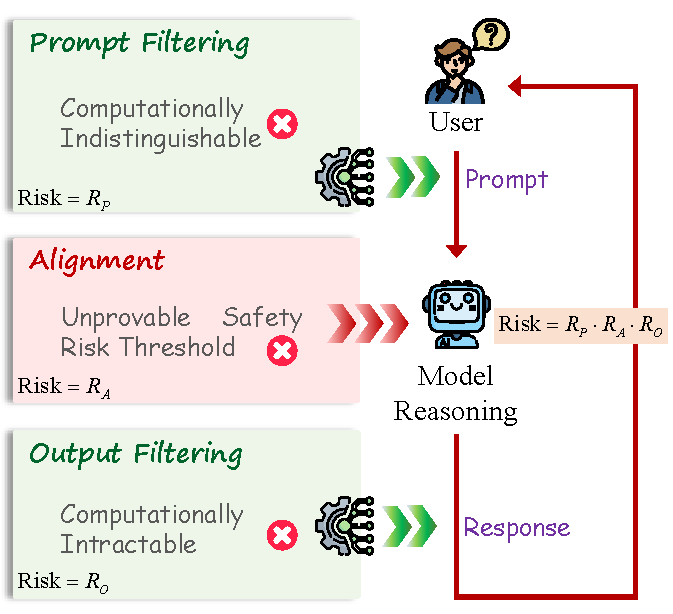
\includegraphics[width=0.97\linewidth]{latex/eval/example.pdf}
    \caption{Overview of security risks in generative model reasoning. These risks arise from the aggregation of risks across three core stages. From a theoretical perspective, such risks are unavoidable.}
    \label{fig:example}   
    \vspace{-15pt}
\end{figure}

With the widespread deployment of generative AI, especially large language models (LLMs), security issues continue to emerge \citep{ji2023beaver, Liu2024injection, Zhan2025CAIS, wang2025uniquesec}. Current AI safety research largely follows a coevolutionary trajectory between attacks and defenses \citep{zhang2025jbshield}. New attack methods and defenses appear continuously. This dynamic leaves existing defenses unprepared for future and unpredictable threats. As a result, the definition of AI safety requires constant revision and expansion. The root cause is inherent risk in model reasoning. This risk is unavoidable and difficult to control, as shown in \autoref{fig:example}. Across the full reasoning pipeline, three stages permit risk intervention. At the model level, emerging threats demand repeated alignment. However, safety fine-tuning \citep{jain2024makes} introduces additional risks, such as backdoor attacks \citep{xu-etal-2024-instructions, wen2024privacy} and data poisoning \citep{chen2024agentpoison}. For external filtering mechanisms, prior work \citep{ball2025impossibility} based on cryptographic hardness shows that efficient prompt filters do not exist for certain large models. Output filtering is computationally intractable. Moreover, some risks remain undetectable \citep{kalai2025consensus}. Therefore, security risk in model reasoning cannot be eliminated. Empirical defenses offer only temporary protection. A generative AI paradigm with provable and controllable risk is therefore necessary. Current research on provably safe AI remains position oriented \citep{dalrymple2024towards}.


Recent work on consensus sampling (CS) \citep{kalai2025consensus} offers partial theoretical control over output risk. CS considers a model group with $s$ safe models and $f$ unsafe models ($s > f$). It exploits overlap among output distributions across models to set the acceptance probability for a response of unknown safety. The goal is to make the delivered response more likely to originate from safe models. The aggregated risk of the group admits a provable upper bound. Unlike prior approaches, CS does not define a safe response. It follows the principle that responses supported by more models carry lower risk. This line of work is orthogonal to empirical safety optimization.

However, CS relies on frequent abstention to avoid unsafe outputs, reducing utility \citep{paulus2025safety}. We further show that adversarial control over unsafe models sharply weakens CS security. Despite a cryptographic upper bound on risk, CS lacks robustness and practicality for deployment.

To address these issues, we propose a new primitive named Reliable Consensus Sampling (RCS). We present a provable safety framework for model groups that includes safety and liveness properties. The definitions draw on classical reliable distributed consensus theory. They enable formal security analysis for model groups. RCS records acceptance probability in real time after sampling failures. After a bounded number of rejections, it enters a trace phase that guarantees eventual delivery of a response. RCS fully avoids abstention. During the trace phase, it reweights model probability distributions to control their influence on the final decision. This design tolerates more extreme adversarial behavior and improves robustness. In addition, inspired by quantum entanglement \citep{nielsen2010quantum}, we introduce a feedback algorithm that captures correlations among model distributions. The algorithm identifies models that are unsafe for sampling on specific tasks. It improves RCS safety by excluding those models from the group decision.

We prove that RCS achieves a controllable risk threshold. Extensive experiments show that RCS significantly improves security and utility compared with CS. Latency remains comparable to CS. We summarize our contributions as follows:  


\begin{itemize}[left=0pt, itemsep=0pt]

\item We define a security property theory for model groups under a Byzantine threat model. The theoretical framework supports provable security analysis.

\item We propose RCS, a trace-based method that eliminates abstention and guarantees eventual delivery. It tracks acceptance probabilities in real time, reweights models to mitigate adversarial influence, and uses a feedback module that exploits cross-model correlations to improve safety.

\item We theoretically prove that RCS admits a tight upper bound on risk. Experiments demonstrate that RCS outperforms CS in robustness and utility while maintaining comparable latency.


\end{itemize}






\section{Preliminary Analysis}



\noindent
\textbf{Notation}.
We follow the notation established in~\citep{kalai2025consensus}. For a prompt $x$, each model $i \in \{1, \dots, n\}$ induces a probability distribution $p_i(y)$ over a output space $\mathcal{Y}$. Let $\mathrm{Distr}(\mathcal{Y})$ denote the set of probability distributions on $\mathcal{Y}$. $\mathcal{Y}$ is the union of the safe space $S$ and the unsafe space $U$. For any $p \in \mathrm{Distr}(\mathcal{Y})$ and any subset $H \subseteq \mathcal{Y}$, we define the cumulative probability $p(H) = \sum_{y \in H} p(y)$. Given a collection of distributions $(p_1, \ldots, p_n) \in \mathrm{Distr}(\mathcal{Y})^n$, let $p_{(i)}(y)$ represent the $i$-th smallest of the probabilities $\{ p_t(y) \}_{t=1}^n$. We use the symbol $\bot \notin \mathcal{Y}$ to denote an abstention. 

\noindent
\textbf{Output Distribution}. Because the model's output is terminated either by special tokens or by a maximum token limit, for a finite tokenizer, We follow existing work \citep{chijiwa2025lossless} to treat the ostensibly unbounded output distribution as a finite set to facilitate analysis. Formally, for model $i$ with maximum token length $L$ and tokenizer $T_i$, the output space is $\mathcal{Y}_i = \bigcup_{j=1}^{L} T_i^j$.


\noindent
\textbf{Model Group}.
The model group ($\mathcal{MG}$) consists of $n$ generative models, including $s$ safe models and 
$f=n-s$ unsafe models. Each safe model should maintain a reasonable probability distribution for any input prompt $x$. The probability that the safety model outputs a safe response is $\Psi > 0$. Unsafe models are assumed to be fully controllable by an adversary and may exhibit arbitrary unsafe behaviors or follow any probability distribution, and we refer to this as the Byzantine model based on the definition of Byzantine replicas in classical BFT consensus research \citep{zhang2023waterbear, dashing2024duan, Das2024AC}.





\section{Reliable Consensus Sampling}
\label{sec:Methodology}


\subsection{Safety Properties}


We define the safety properties in $\mathcal{MG}$ based on the definitions from reliable distributed systems \citep{cachin2011introduction}.

\noindent
\textbf{Safety}. Let $f < \lceil \frac{n}{2} \rceil$, at all times, the risk of the model group $q(U) \leq n \cdot \mu(U) + \mathrm{negl}(\lambda)$. $\mu(U)$ is the average risk of generating unsafe response $y \in U$ by $s$ safe models. Safety requires that the risk of unsafe models is reduced to the risk of safe models plus $\mathrm{negl}(\lambda)$. $\lambda$ is a security parameter.

\noindent
\textbf{Liveness}. The liveness property requires that, for any time $t$, there remains the hope that the property will be satisfied at some later time $t' \ge t$. The mechanism must still retain the possibility of eventually delivering a usable response $y \in \mathcal{Y}$, although it may be risky. Liveness reflects the utility of $\mathcal{MG}$.



\noindent
\textbf{Anti-Collusion}.
$\mathcal{MG}$ must tolerate arbitrary behavior from up to $f$ Byzantine models. Such behavior includes full control over the probability distribution of $y \in \mathcal{Y}$. This control may assign low probability to safe responses. It may also assign high probability to unsafe responses. These behaviors should not significantly affect the safety of the response delivered by $\mathcal{MG}$.


\noindent
\textbf{Half-Resilience}. In real-world deployments, the values of $s$ and $f$ may change over time. We consider a time $t$ at which $m$ out of the $s$ safe models become unsafe. The $\mathcal{MG}$ system then transitions to a new state with $s' = s - m$ and $f' = f + m$. In this state, the condition $f < \lceil \frac{n}{2} \rceil$ no longer holds. We do not require $\mathcal{MG}$ to preserve theoretical safety or liveness. Instead, we require the system to remain practically robust and avoid catastrophic failure. In this paper, we focus on the case of $f=s$.


\noindent
\textbf{Termination}. 
The algorithm is guaranteed to complete within a finite time $T$.


\subsection{Methodology}
Our proposed RCS scheme is shown in Algorithm \ref{alg:consensus}. During the $R$ rounds of sampling, in each round, if the candidate response $y$ is not accepted, we record $y$ and its acceptance probability $\sigma(y)$ in real time. When all $R$ sampling rounds fail, the protocol enters the trace phase. In this phase, we select the top $\min(s, R)$ values of $\sigma(y)$ and collect the corresponding $y$ into the set $\mathcal{F}$. For each $y \in \mathcal{F}$, we compute $\alpha(y)$ as the sum of the largest $n - s$ values in $\{p_j(y)\}_{j=1}^{n}$, which have already been obtained during the computation of $\sigma(y)$. We then select the $y$ with the largest $\alpha(y)$ in order to mitigate the impact of Byzantine models, while maintaining the liveness guarantee.


\begin{algorithm}[t]
\SetAlgoLined
\KwIn{
Number of models $|\mathcal{MG}|=n$; number of safe models $s$; 
round $R$; distributions $p_1, \ldots, p_n \in \mathrm{Distr}(\mathcal{Y})^{n}$
}
\KwOut{Response $y \in \mathcal{Y}$}

$Buffer \gets \varnothing$\\
\For{$r \leftarrow 1$ \KwTo $R$}{
    Sample $y \sim \frac{1}{n}\sum_{i=1}^{n} p_i$ \\
    $\sigma(y) =\frac{\frac{1}{s}\sum_{i=1}^{s} p_{(i)}(y)}
             {\frac{1}{n}\sum_{i=1}^{n} p_i(y)}$
        
    \If{accept $y$ with $\sigma(y)$}{
        \Return $y$
    }
    $Buffer \gets Buffer \cup \{\langle y, \sigma(y) \rangle \}$\\
}

Sort $Buffer=\{\langle y_i, \sigma(y_i) \rangle \}_{i=1}^{R}$ 
 such that $\sigma(y_{(1)}) \ge \dots \ge \sigma(y_{(R)})$\\
Let $\mathcal{F} = \{y_{(1)}, \dots, y_{u}\}, \; u= min(s,R)$ \\
\For{$i \leftarrow 1$ \KwTo $u$}{
    $\alpha(y_{(i)}) = \sum_{j=s+1}^{n} p_{(j)}(y_{(i)})$
}
\Return $y \gets \arg\max_{y \in \mathcal{F}} \alpha(y)$

\caption{Reliable Consensus Sampling Algorithm}
\label{alg:consensus}
\end{algorithm}



We present a rigorous theoretical proof of the safety property of RCS. The overlap of the output probability distributions of the $s$ safest models, that is, their degree of consensus, is computed by using $Z = \sum_{y}\frac{1}{s}\sum_{i=1}^{s}p_{(i)}(y)$ \citep{kalai2025consensus}. We denote $\Pr[T]=(1-Z)^R$ as the probability of entering the trace phase, and $\rho(U)$ as the probability that the trace phase eventually outputs an unsafe response. Let $R = \mathrm{poly}(\lambda)$. Then the risk of RCS satisfies:

\begin{align*}
q(U) &= (1-\Pr[\text{T}]) \cdot \frac{1}{Z} \sum_{y \in U}\frac{1}{s}\sum_{i=1}^{s}p_{(i)}(y) \\ &+ \Pr[\text{T}] \cdot \rho(U)\\
&\leq  ZR \cdot \frac{1}{Z} \sum_{y \in U}\frac{1}{s}\sum_{i=1}^{s}p_{(i)}(y) + \Pr[\text{T}] \cdot \rho(U)\\
&=  R \cdot \sum_{y \in U}\frac{1}{s}\sum_{i=1}^{s}p_{(i)}(y) + \Pr[\text{T}] \cdot \rho(U)\\
&\leq R \cdot \frac{1}{s}\sum_{i=1}^{s}p_{(i)}(U) + \Pr[\text{T}] \cdot \rho(U) \\
&= R \cdot\mu(U) + (1-Z)^R \cdot \rho(U)
\end{align*}

In $\mathcal{MG}$, at least $s - f$ values of $p_i(y)$ satisfy $p_i(y) > 0$. Therefore, $Z > 0$. It follows that
$(1-Z)^R = e^{R \ln(1-Z)}$. Since $\ln(1-Z) < 0$, $\rho(U) \in (0,1)$ and $R = \mathrm{poly}(\lambda)$, we have $(1-Z)^R \cdot \rho(U) = \mathrm{negl}(\lambda)$. Therefore, $q(U) \leq R \cdot \mu(U) + \text{negl}(\lambda)$. We set the upper bound as $n = k R + b$, where $k,b > 0$ are constants. Under this choice, for any $R \le n$, $q(U) \le n \cdot \mu(U) + \mathrm{negl}(\lambda)$ holds. In fact, the above proof involves two equality conditions. These conditions are difficult to satisfy simultaneously. The first condition is $R = 1$. This condition can be enforced by design. The second condition requires that for all $y \in U$,
$p_i(y) \le p_j(y), \; \forall i \in S,\; j \notin S .$
This condition is extremely difficult to satisfy in practice. Therefore, in general, we have $q(U) < n \cdot \mu(U) + \mathrm{negl}(\lambda)$. As $R \to +\infty$ (without considering termination), we have $\Pr[T] \to 0$, indicating that $\mathcal{MG}$ delivers a response with probability approaching unity. In this asymptotic regime, the condition $q(U) \le n \cdot \mu(U)$ remains valid, thereby ensuring the safety property.



\subsection{Analysis}
We provide a comprehensive comparison between RCS and existing CS method in \autoref{tab:compare}. Below, we analyze each property in detail.

\begin{table*}
\centering
 \scalebox{0.75}{
    \begin{tabular}{@{}l|cccccc@{}}
    \toprule
\textbf{Algorithm}  & \textbf{Safety} & \textbf{Liveness} & \textbf{Anti-Collusion} & \textbf{Half-Resilience} & \textbf{Termination} &\textbf{Time Complexity}\\
    \midrule
Consensus Sampling & \textcolor{nGreen}{\ding{51}} & \textcolor{nRed}{\ding{55}} & \textcolor{nRed}{\ding{55}} & \textcolor{nRed}{\ding{55}} & \textcolor{nGreen}{\ding{51}} & $\mathcal{O}(RI)$\\
Reliable Consensus Sampling & \textcolor{nGreen}{\ding{51}} & \textcolor{nGreen}{\ding{51}} & \textcolor{nGreen}{\ding{51}} & \textcolor{nGreen}{\ding{51}} & \textcolor{nGreen}{\ding{51}} & $[\mathcal{O}(RI), \ \mathcal{O}(RI + n^2 \log n)]$\\
    \bottomrule
    \end{tabular}
 }
 \caption{A comprehensive comparison between our proposed RCS and existing method.}
    \label{tab:compare}
\end{table*}


\noindent
\textbf{Latency}. Let $I$ denote the time required to sample $y$ from a distribution $p_i$.
In RCS, if no sample is accepted after $R$ rounds, the algorithm incurs an additional cost of $n^2 \log n$ for trace computation. This cost is negligible compared with $I$, especially for reasoning LLMs \citep{chen2025towards}. Therefore, RCS and CS have comparable time complexity.



\noindent
\textbf{Anti-Collusion}. The goal of collusion is to make $\mathcal{MG}$ more likely to deliver unsafe responses by manipulating one or more Byzantine models. We study the relation between acceptance probabilities of an unsafe response $y_t$ and a safe response $y_v$ within the $R$ round loop of Algorithm \ref{alg:consensus}. We focus on the quantity $\Delta(\sigma) = \sigma(y_t) - \sigma(y_v)$. The detailed derivation appears in \autoref{app:ac}. The sign of $\Delta(\sigma)$ depends on:
\[
\mathcal{D}_{t,v} =
\frac{
\sum_{i = 1}^{s} p_{(i)}(y_t) \sum_{i = s+1}^{n} p_{(i)}(y_v)
}{
\sum_{i = 1}^{s} p_{(i)}(y_v) \sum_{i = s+1}^{n} p_{(i)}(y_t)
}.
\]

When the Byzantine model assigns a very low probability to $y_v$, the value of
$\sum_{i=1}^{s} p_{(i)}(y_v)$ decreases, leading to $\mathcal{D}_{t,v} > 1$. As a result, $\Delta(\sigma) > 0$, which significantly increases the acceptance probability of the unsafe response $y_t$ relative to $y_v$. This effect weakens the security of $\mathcal{MG}$. When unsafe models collude, we present the resulting model probability distributions in \autoref{fig:distribution}. The adversarial behavior of unsafe models clearly has a significant impact on the probability overlap among models in CS. In contrast, the design in lines 9-12 of Algorithm \ref{alg:consensus} effectively mitigates this issue. When the values of $p_{\text{unsafe}}(y_v)_j$ are very low, RCS can significantly downweight their influence on the final output response.



\begin{figure*}[!]
    \centering
    \begin{subfigure}{0.48\textwidth}
        \centering
        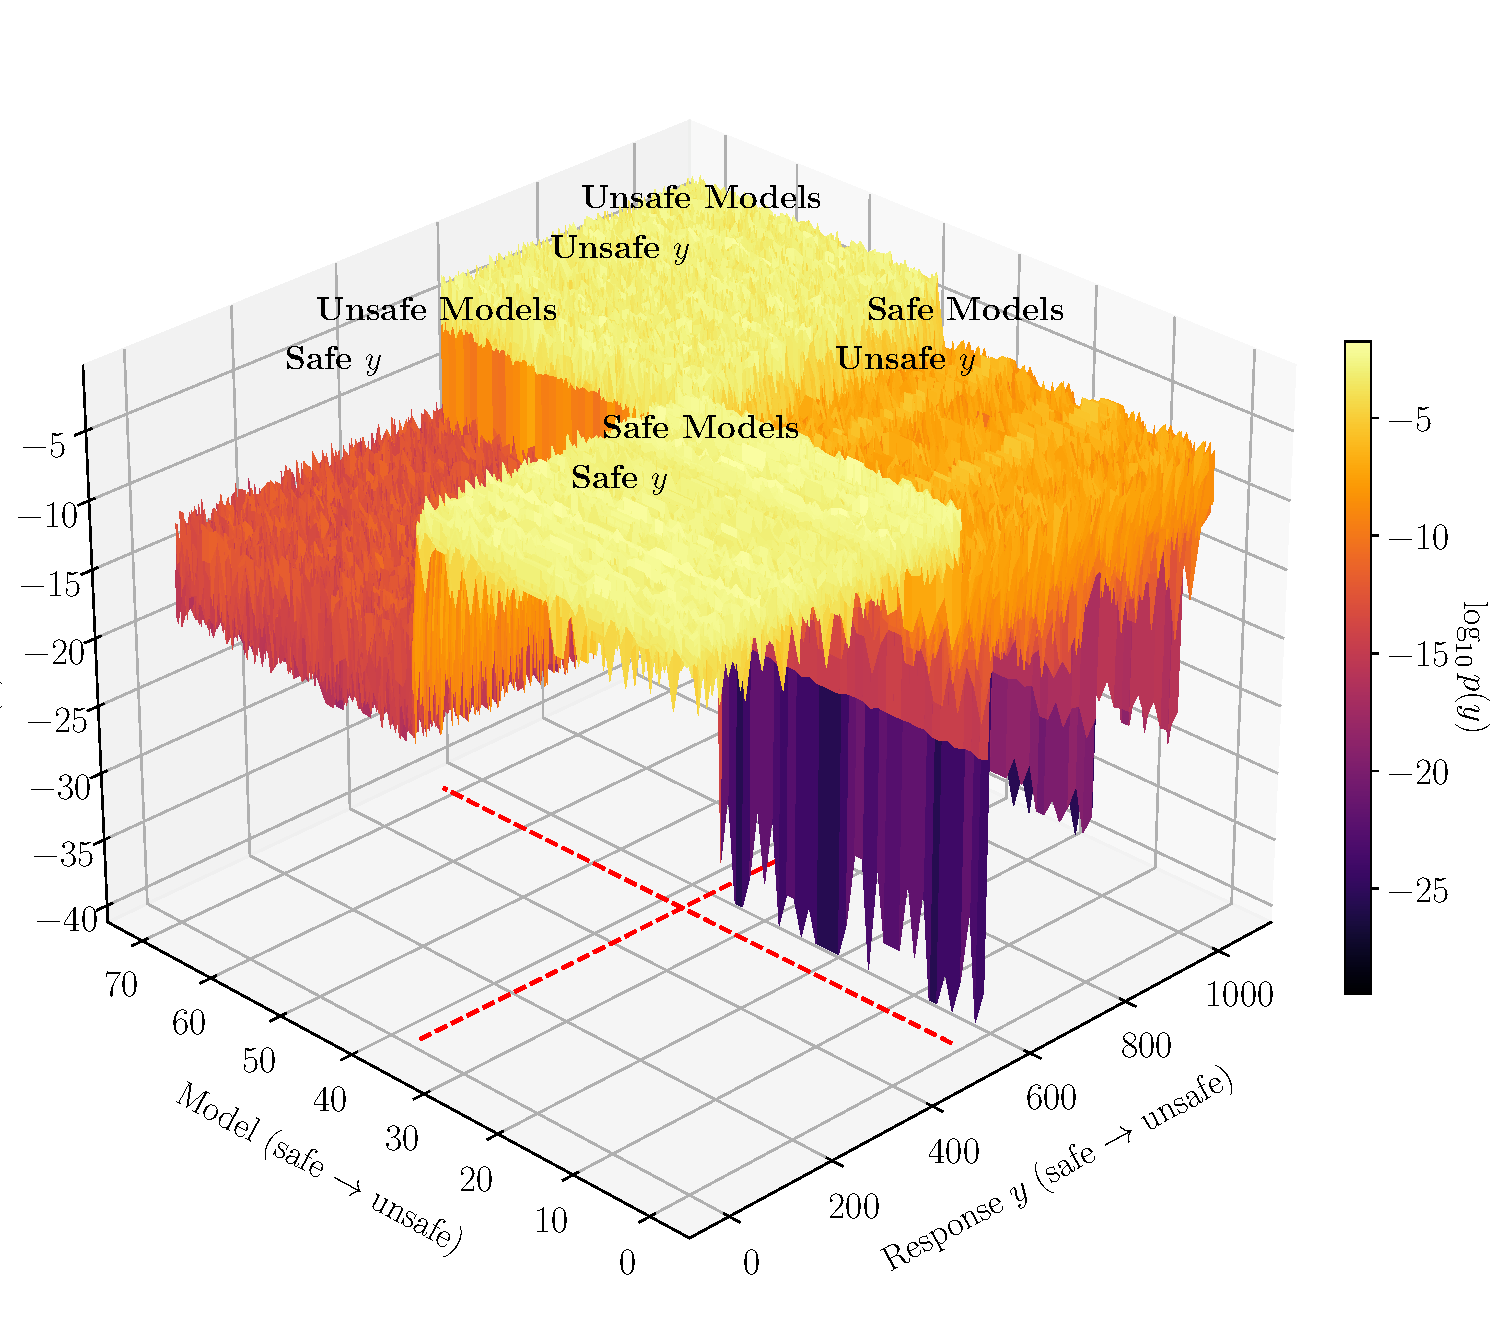
\includegraphics[width=\linewidth]{latex/eval/distribution.pdf}
        \caption{Distribution under general adversarial conditions.}
    \end{subfigure}
    % \hspace{40pt}
    \begin{subfigure}{0.48\textwidth}
        \centering
        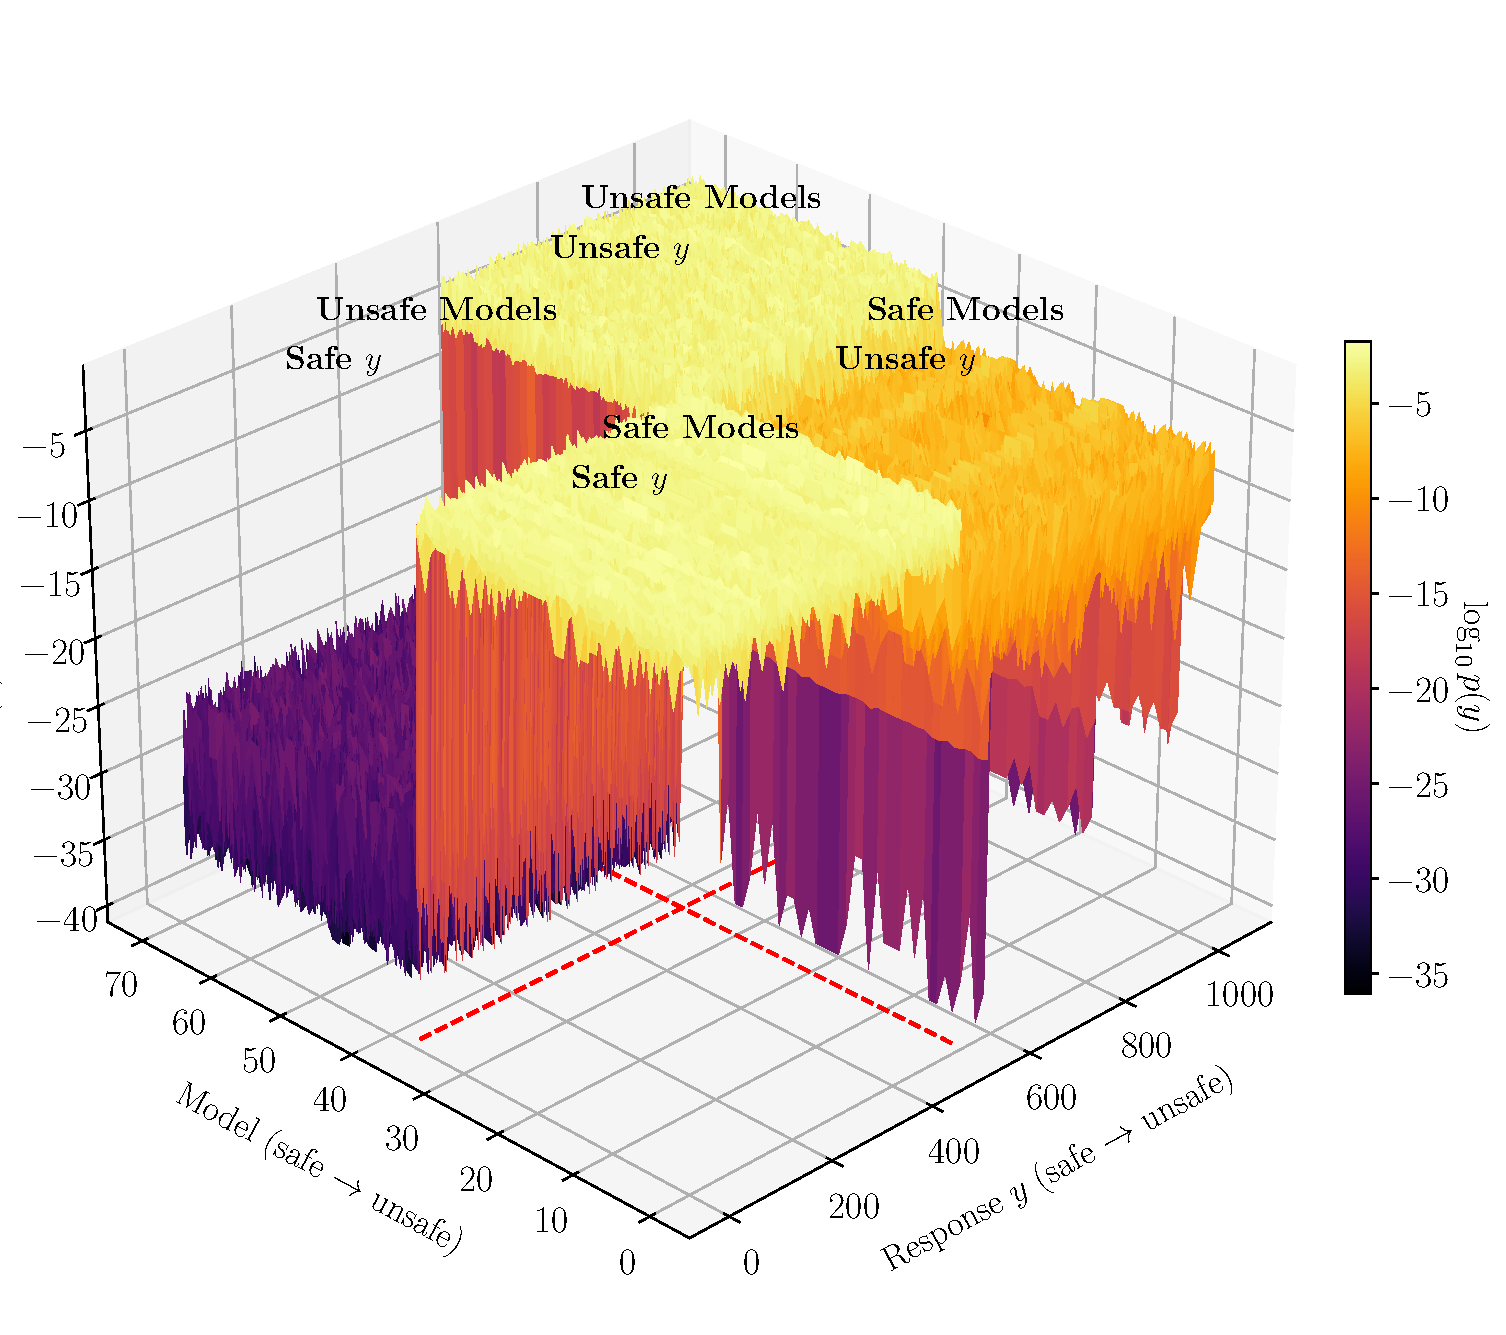
\includegraphics[width=\linewidth]{latex/eval/distribution2.pdf}
        \caption{Distribution under malicious collusion.}
    \end{subfigure}
    \caption{Model probability distribution for consensus sampling under diverse adversarial environments.}
    \label{fig:distribution}
    \vspace{-15pt}
\end{figure*}




\noindent
\textbf{Half-Resilience}. The CS algorithm has an abstention bound, meaning $\Pr[y=\bot]$ does not exceed a threshold when $f < \lceil \frac{n}{2} \rceil$. However, if this condition is violated, the CS abstention bound is affected, leading to an increased probability of abstention and a significant impact on liveness. RCS can avoid this issue. We further validate the half-resilience of RCS in the experiments in Section \ref{sec:experiment}.

\noindent
\textbf{Termination}. 
According to Algorithm \ref{alg:consensus}, for a finite $R$, RCS always terminates within $R$ rounds.





\section{Feedback-Optimized Reliable Consensus Sampling}
For CS and RCS, the framework does not require an explicit definition of security properties. This design allows algorithms to remain applicable over time. From this perspective, for each concrete task, one cannot determine the probability that the final delivered result is safe. This holds even though the algorithmic risk admits an upper bound. External control over the sampling process is limited. This implies that, from both an algorithmic and long-term operational perspective, if the $\mathcal{MG}$ remains unchanged and the input task types are essentially fixed, the risk in RCS remains stationary over time, thereby limiting the potential for dynamic optimization. In this section, we analyze the nature of response safety in RCS. Inspired by quantum computing \citep{nielsen2010quantum}, we propose a research methodology for RCS based on quantum states. We further introduce a mechanism that intervenes in model distributions and dynamically improves safety.


\subsection{Foundational Theory}
\label{sec:Theory}
\noindent
Motivated by quantum computation theory, we propose a framework for studying the security of RCS by analogy with quantum theory.

\noindent
\textbf{Understanding RCS Safety from a Quantum State Perspective}. 
We model a system with unknown safety as a quantum state $|\phi\rangle$, defined as
$|\phi\rangle = \alpha |0\rangle + \beta |1\rangle$,
where $|0\rangle$ denotes a safe state and $|1\rangle$ denotes an unsafe state. The constraint $\alpha^2 + \beta^2 = 1$ holds. Before evaluation, $|\phi\rangle$ does not reside in a definite safe or unsafe state. It remains in a superposition, analogous to Schr\"odinger's cat. The value $|\alpha|^2$ denotes the probability of safety, while $|\beta|^2$ denotes the probability of unsafety.

Given a fixed prompt $q$ and an evaluation method $e$, we apply $\mathrm{Eval}(q, |\phi\rangle, e)$. The state $|\phi\rangle$ then collapses to $|0\rangle$ or $|1\rangle$. Only at this stage can one determine safety under $q$ and $e$. Therefore, $|\phi\rangle$ alone cannot be labeled as safe or unsafe. The state becomes concrete only under the joint action of $q$ and $e$. The desired condition is $|\alpha| > |\beta|$, meaning a stronger bias toward the safe state.

\noindent
\textbf{Entanglement Theory for RCS}. Consider an $\mathcal{MG}$ with $n$ models $\{|\phi_1\rangle, |\phi_2\rangle, \dots, |\phi_n\rangle\}$. In each sampling round, the randomly selected model $|\phi_r\rangle$ remains in a superposition of safety and unsafety. However, the response $y$ produced by $|\phi_r\rangle$ implicitly links $|\phi_r\rangle$ with other models. In $\mathcal{MG}$, there exists a subset
$W = \{|\phi_1\rangle, |\phi_2\rangle, \dots, |\phi_\ell\rangle\}$
that assigns a high probability to $y$. There also exists a subset
$X = \{|\phi_{\ell+1}\rangle, |\phi_{\ell+2}\rangle, \dots, |\phi_n\rangle\}$
that assigns a low probability to $y$. The model $|\phi_r\rangle$ belongs to neither $W$ nor $X$. We say that $W$ and $X$ are entangled. After a time interval $\Delta(t)$, suppose evaluation under $q$ and $e$ verifies that $|\phi_r\rangle$ is unsafe. Then models in $W$ are likely unsafe, while models in $X$ are likely safe. In subsequent sampling, when a prompt $x$ and an evaluation $a$ resemble $q$ and $e$, the algorithm should increase weights for models in $X$ and decrease weights for models in $W$.






\begin{figure*}[!]
    \centering
    \begin{subfigure}{0.31\textwidth}
        \centering
        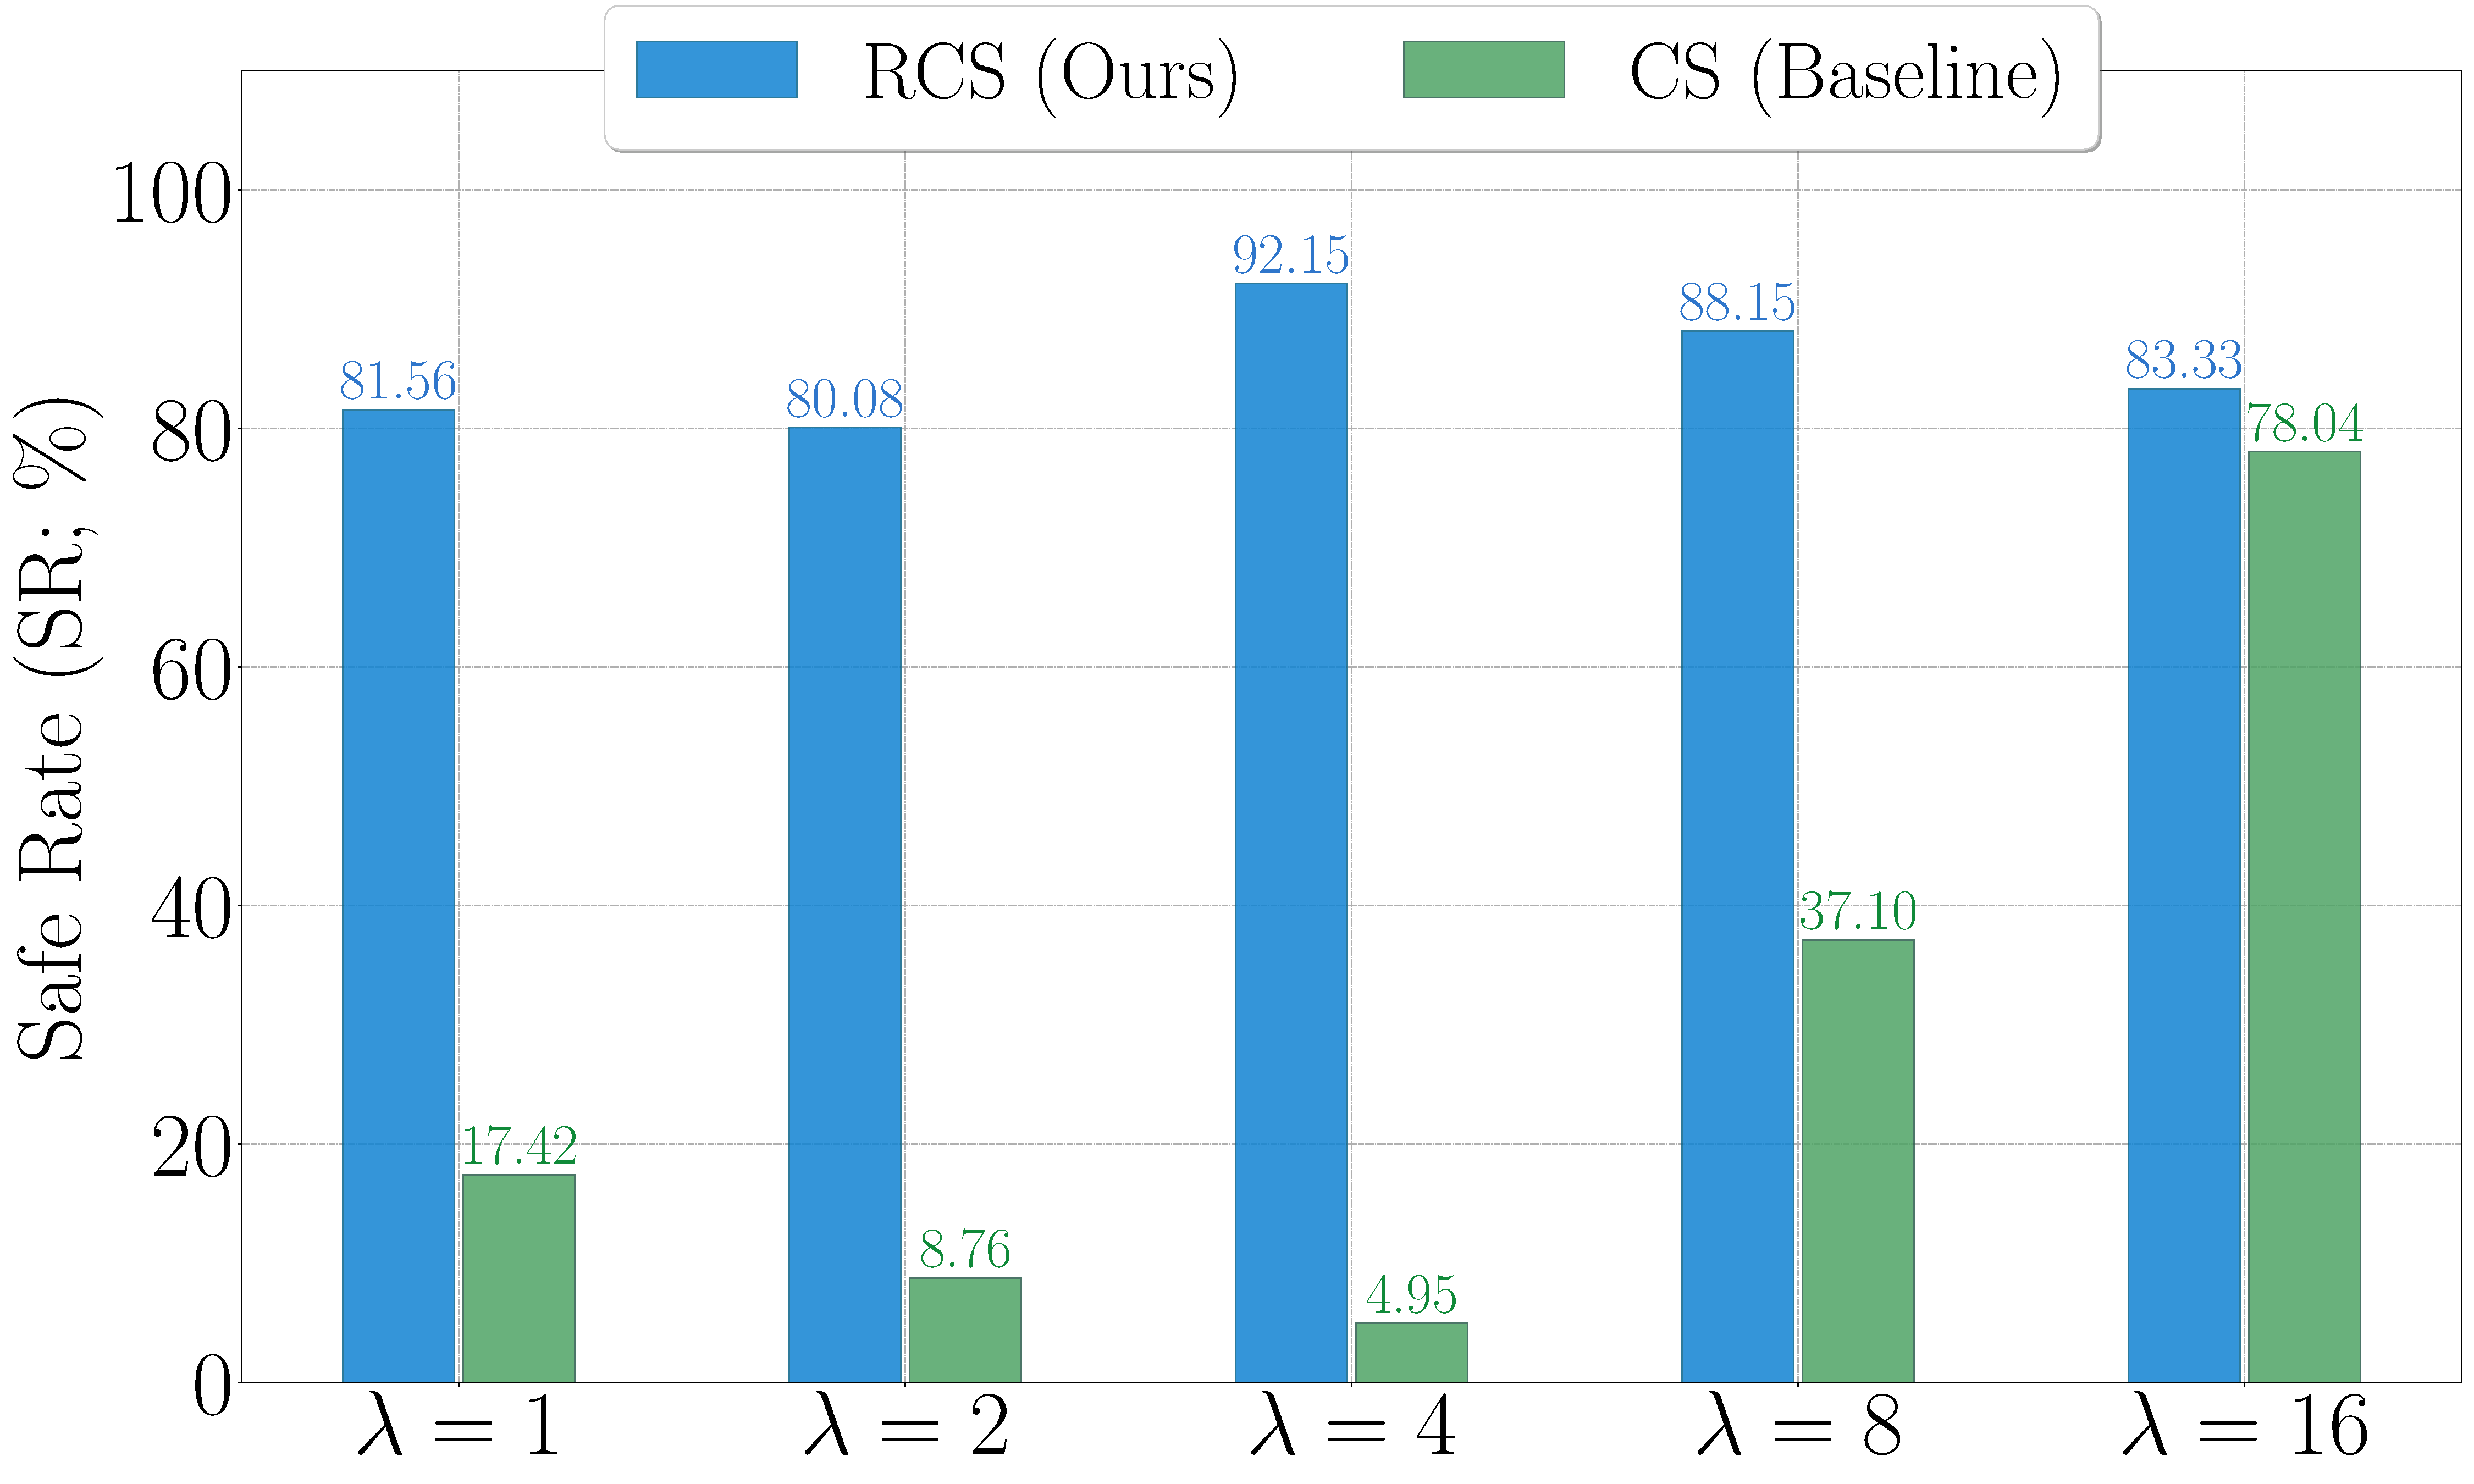
\includegraphics[width=\linewidth]{latex/eval_res/SR-33.pdf}
        \caption{$n=33$.}
    \end{subfigure}
    \begin{subfigure}{0.31\textwidth}
        \centering
        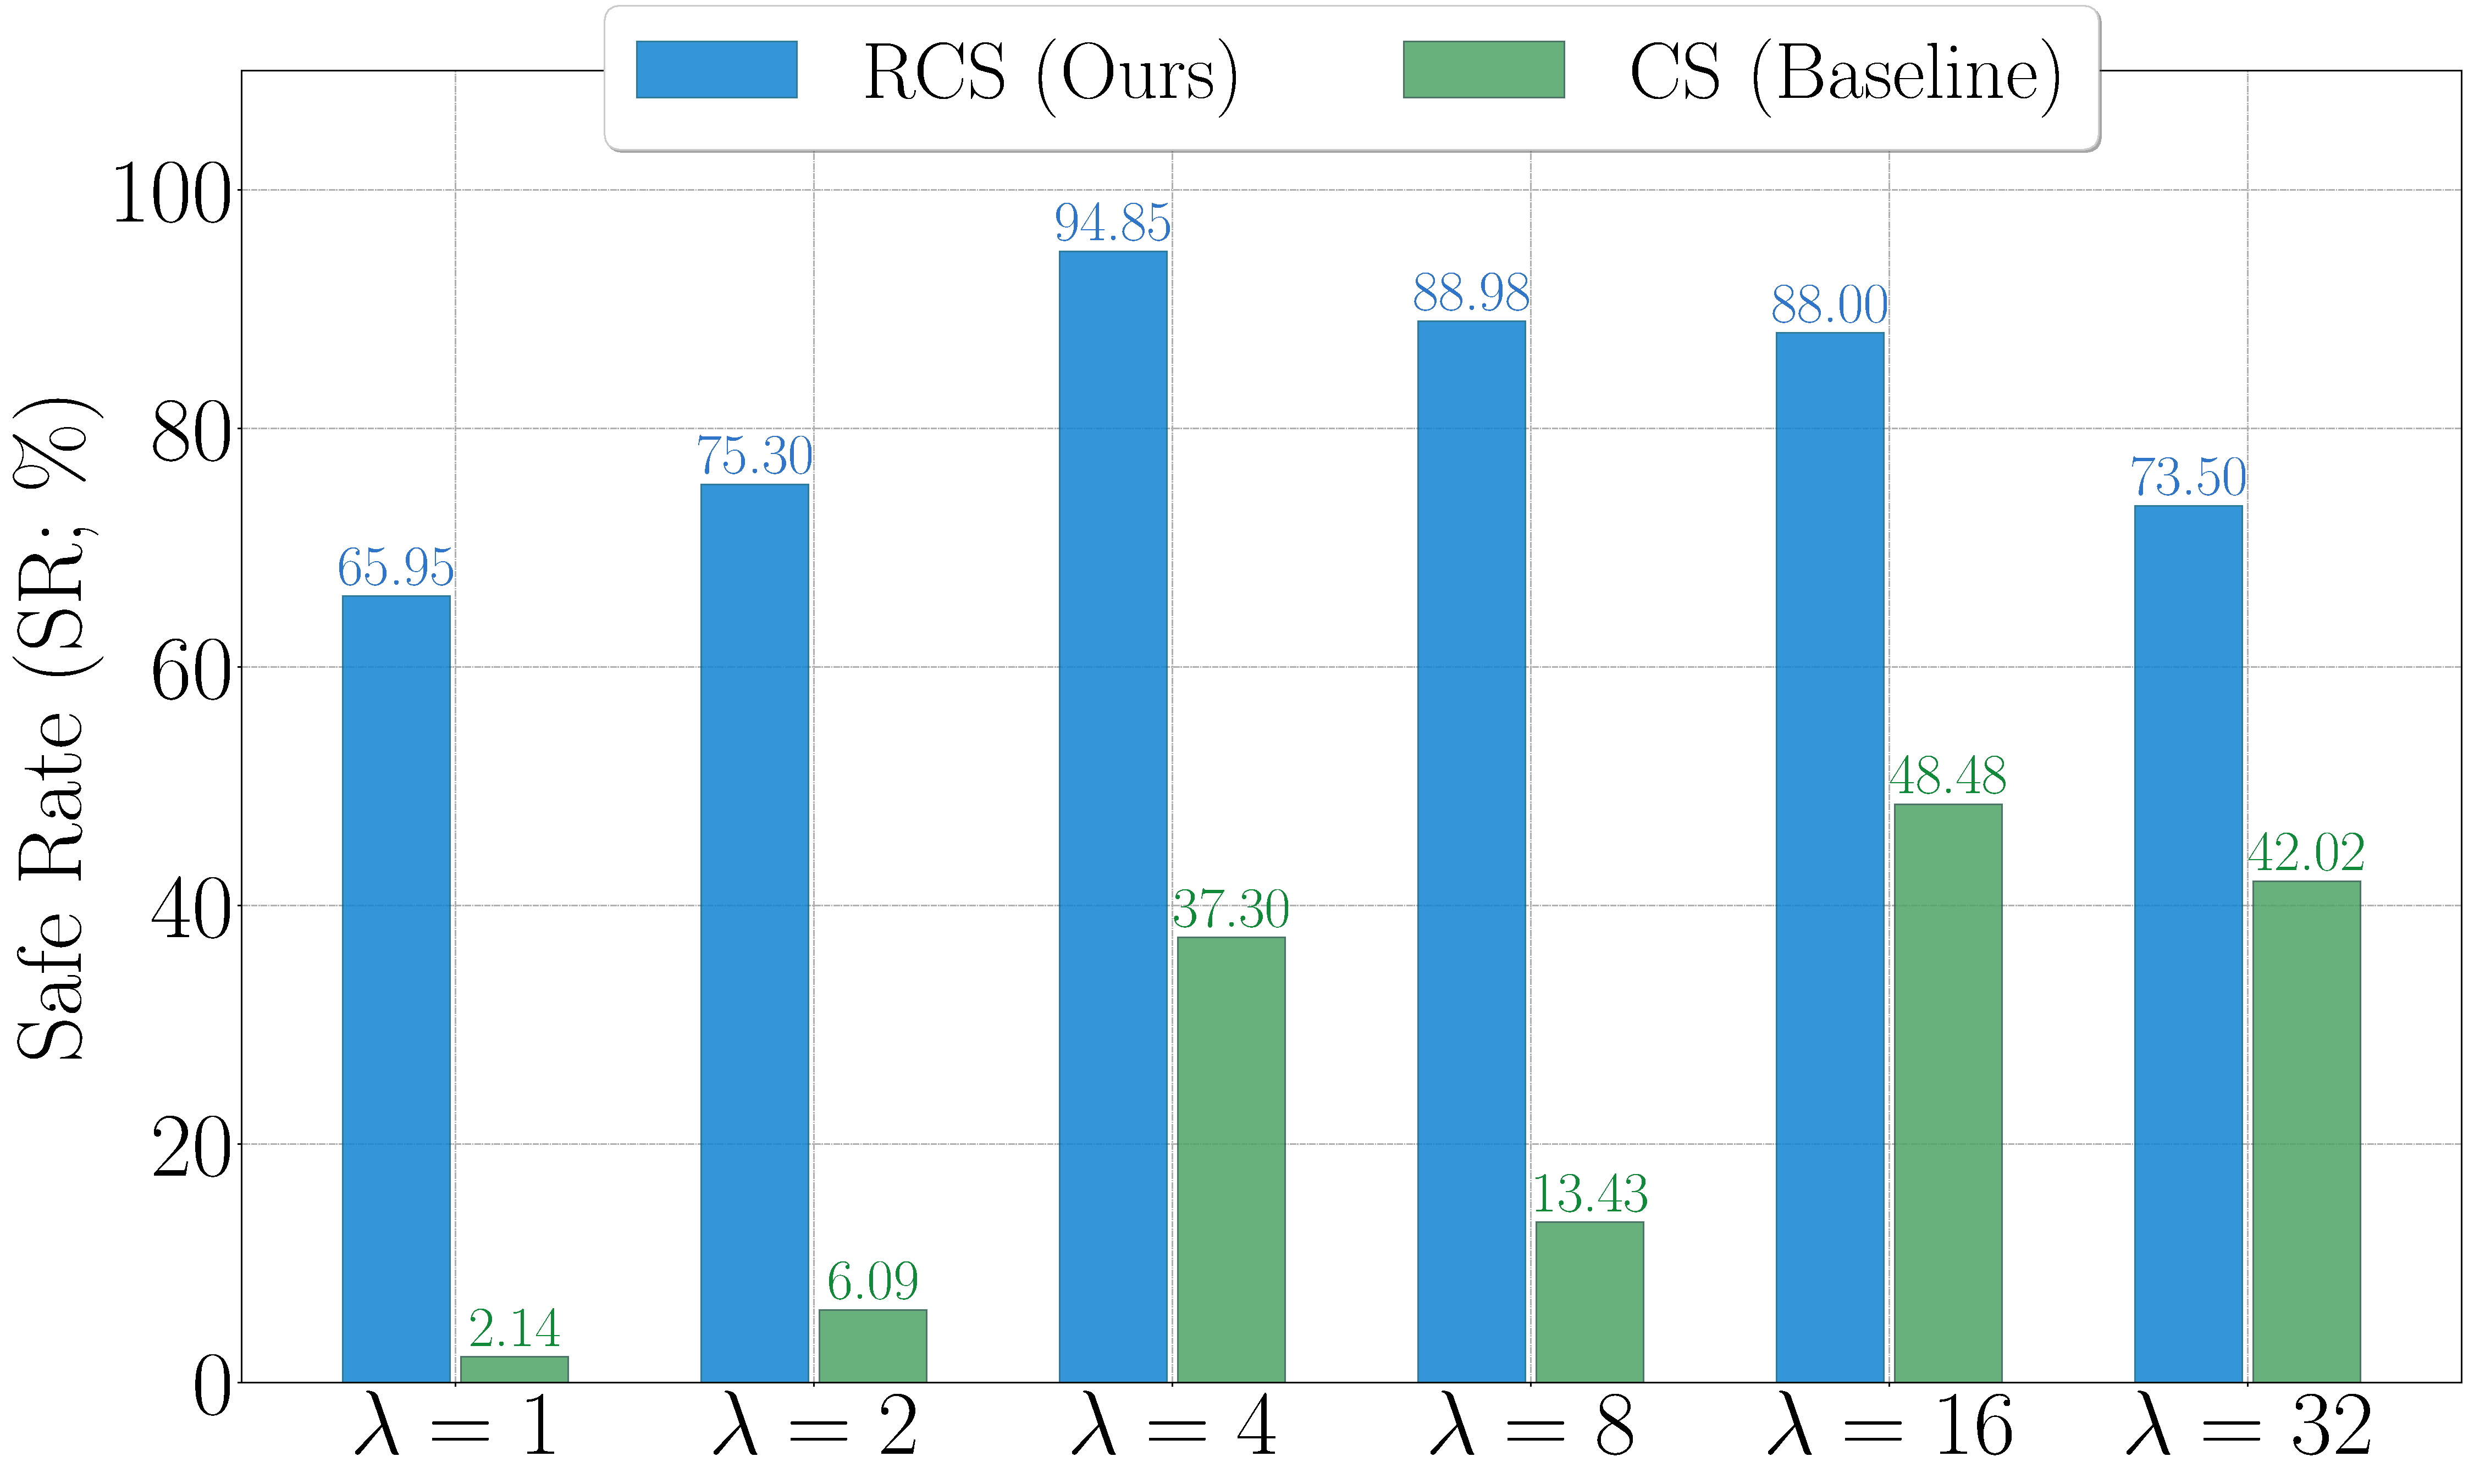
\includegraphics[width=\linewidth]{latex/eval_res/SR-65.pdf}
        \caption{$n=65$.}
    \end{subfigure}
    \begin{subfigure}{0.31\textwidth}
        \centering
        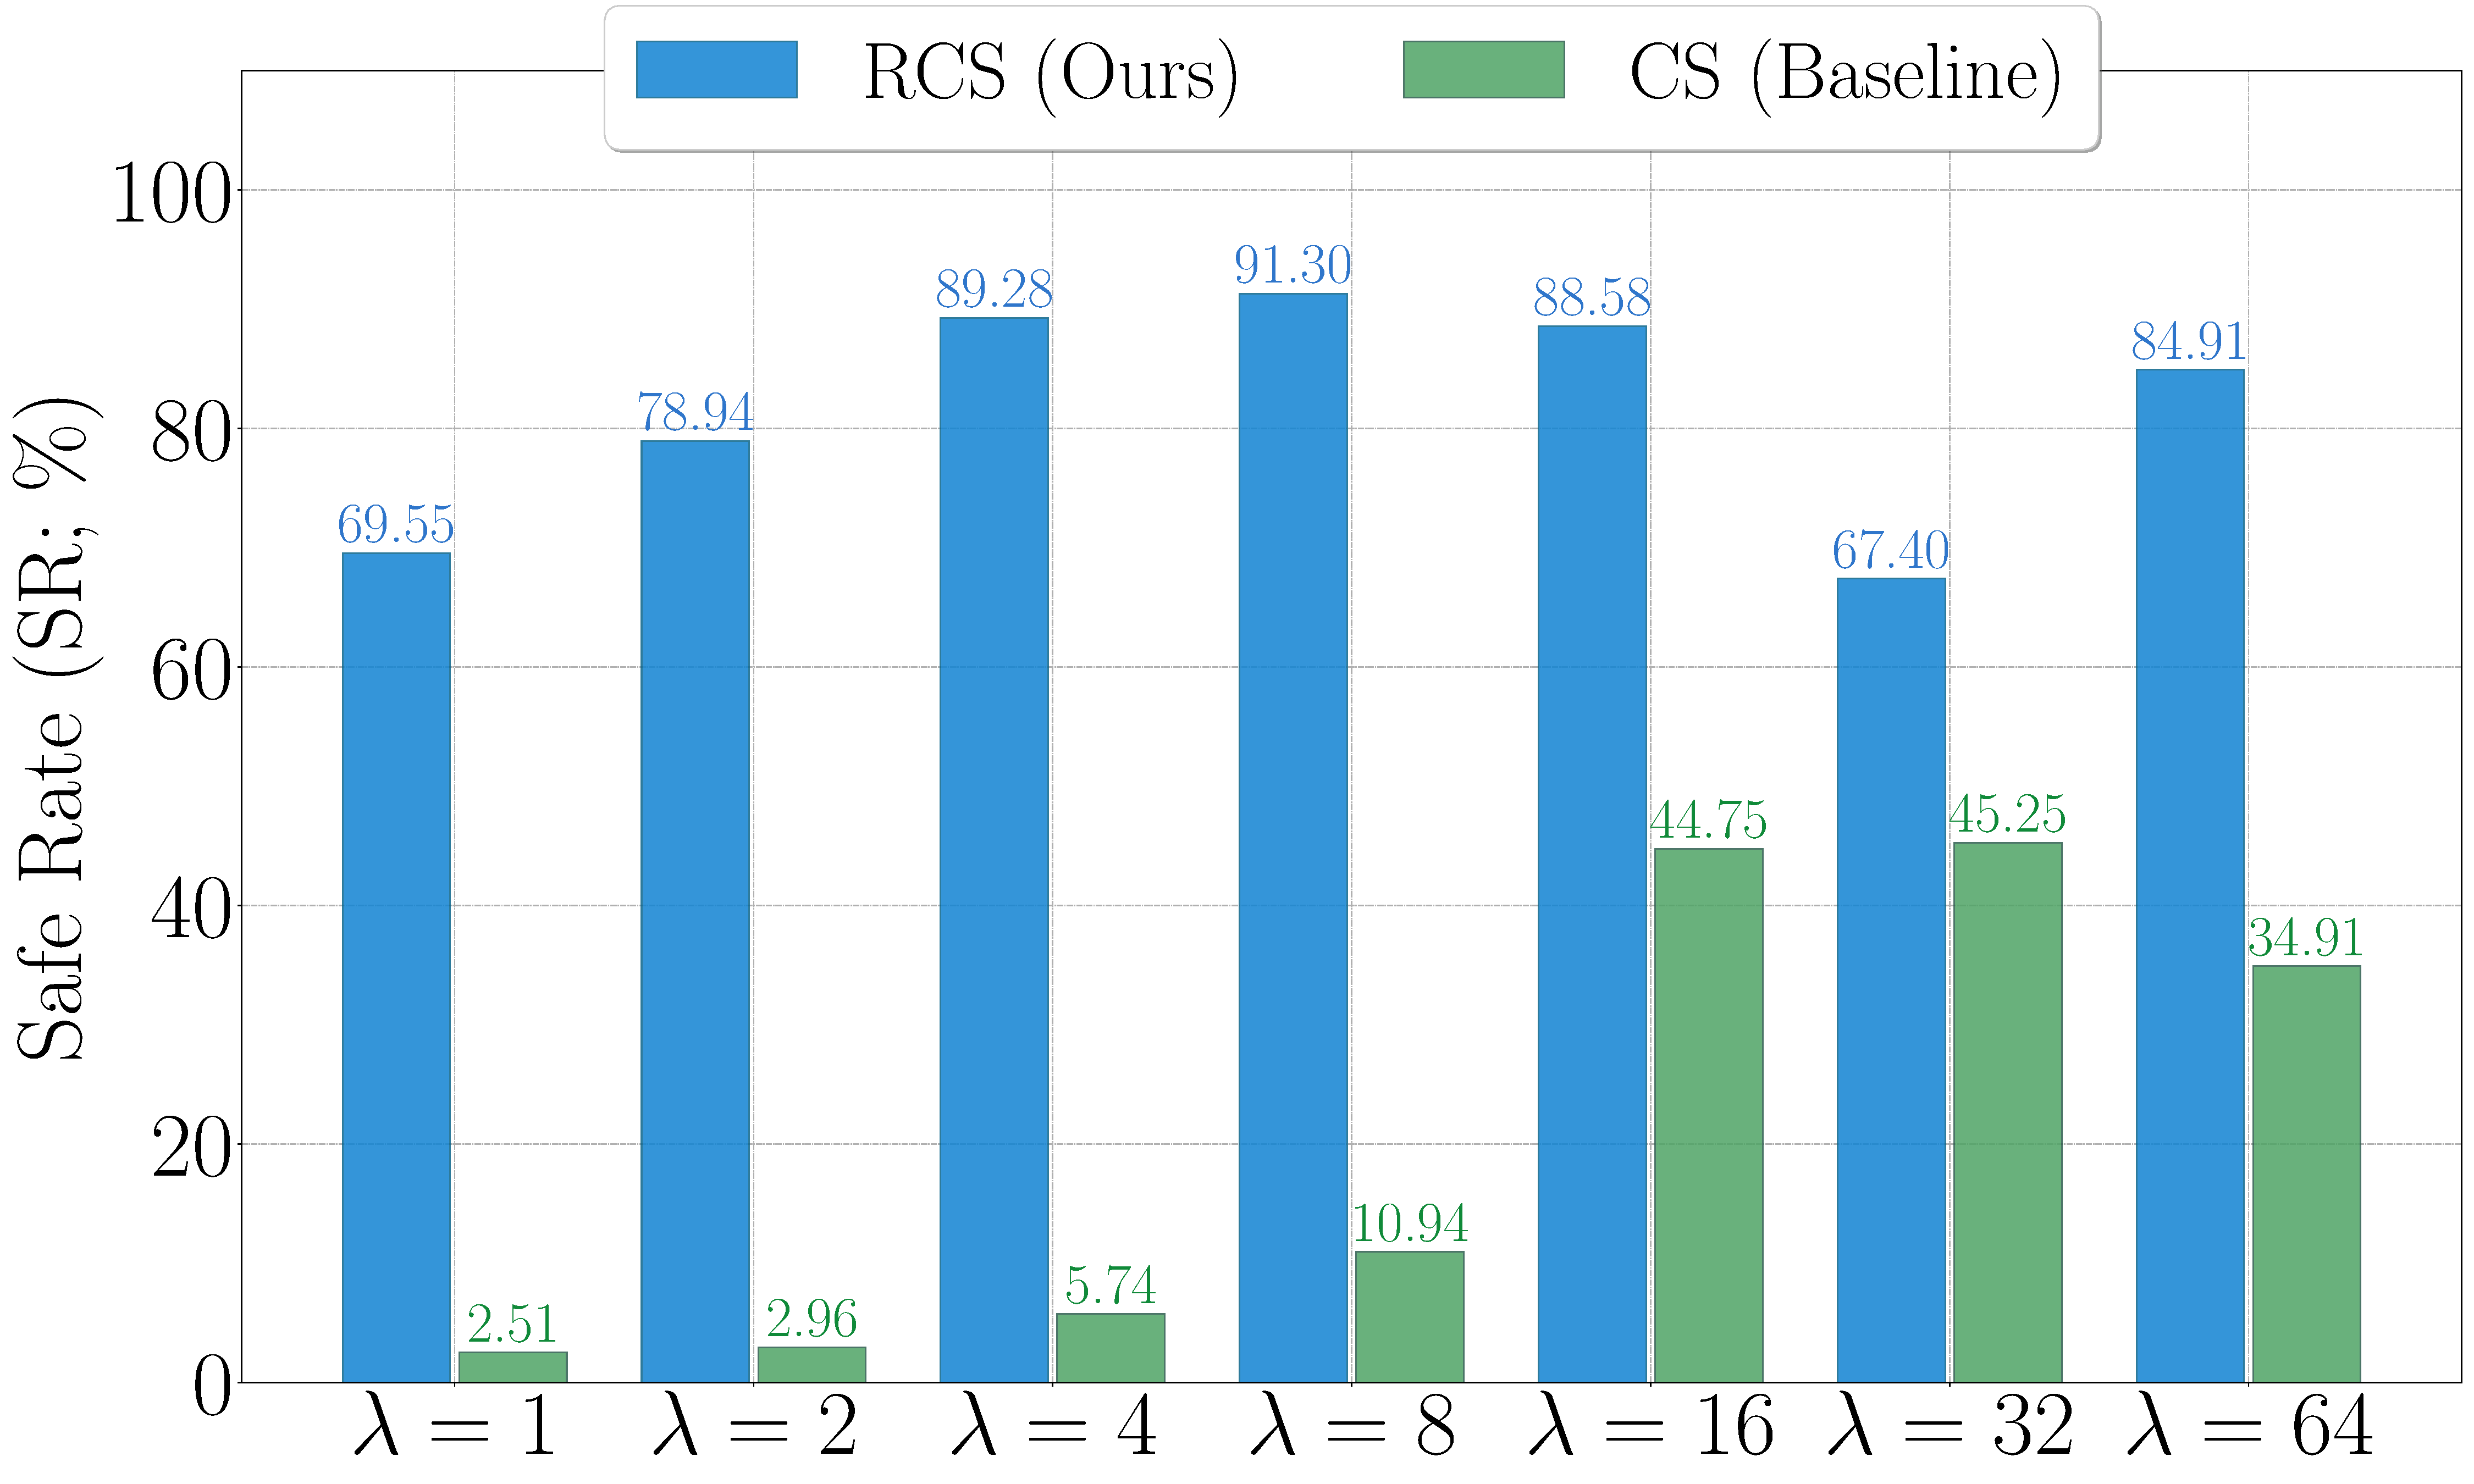
\includegraphics[width=\linewidth]{latex/eval_res/SR-129.pdf}
        \caption{$n=129$.}
    \end{subfigure}
    \caption{Evaluation results for the safe rate when $f < \lceil \frac{n}{2} \rceil$.}
    \label{fig:SR_g}
    % \vspace{-15pt}
\end{figure*}



\begin{figure*}[!]
    \centering
    \begin{subfigure}{0.31\textwidth}
        \centering
        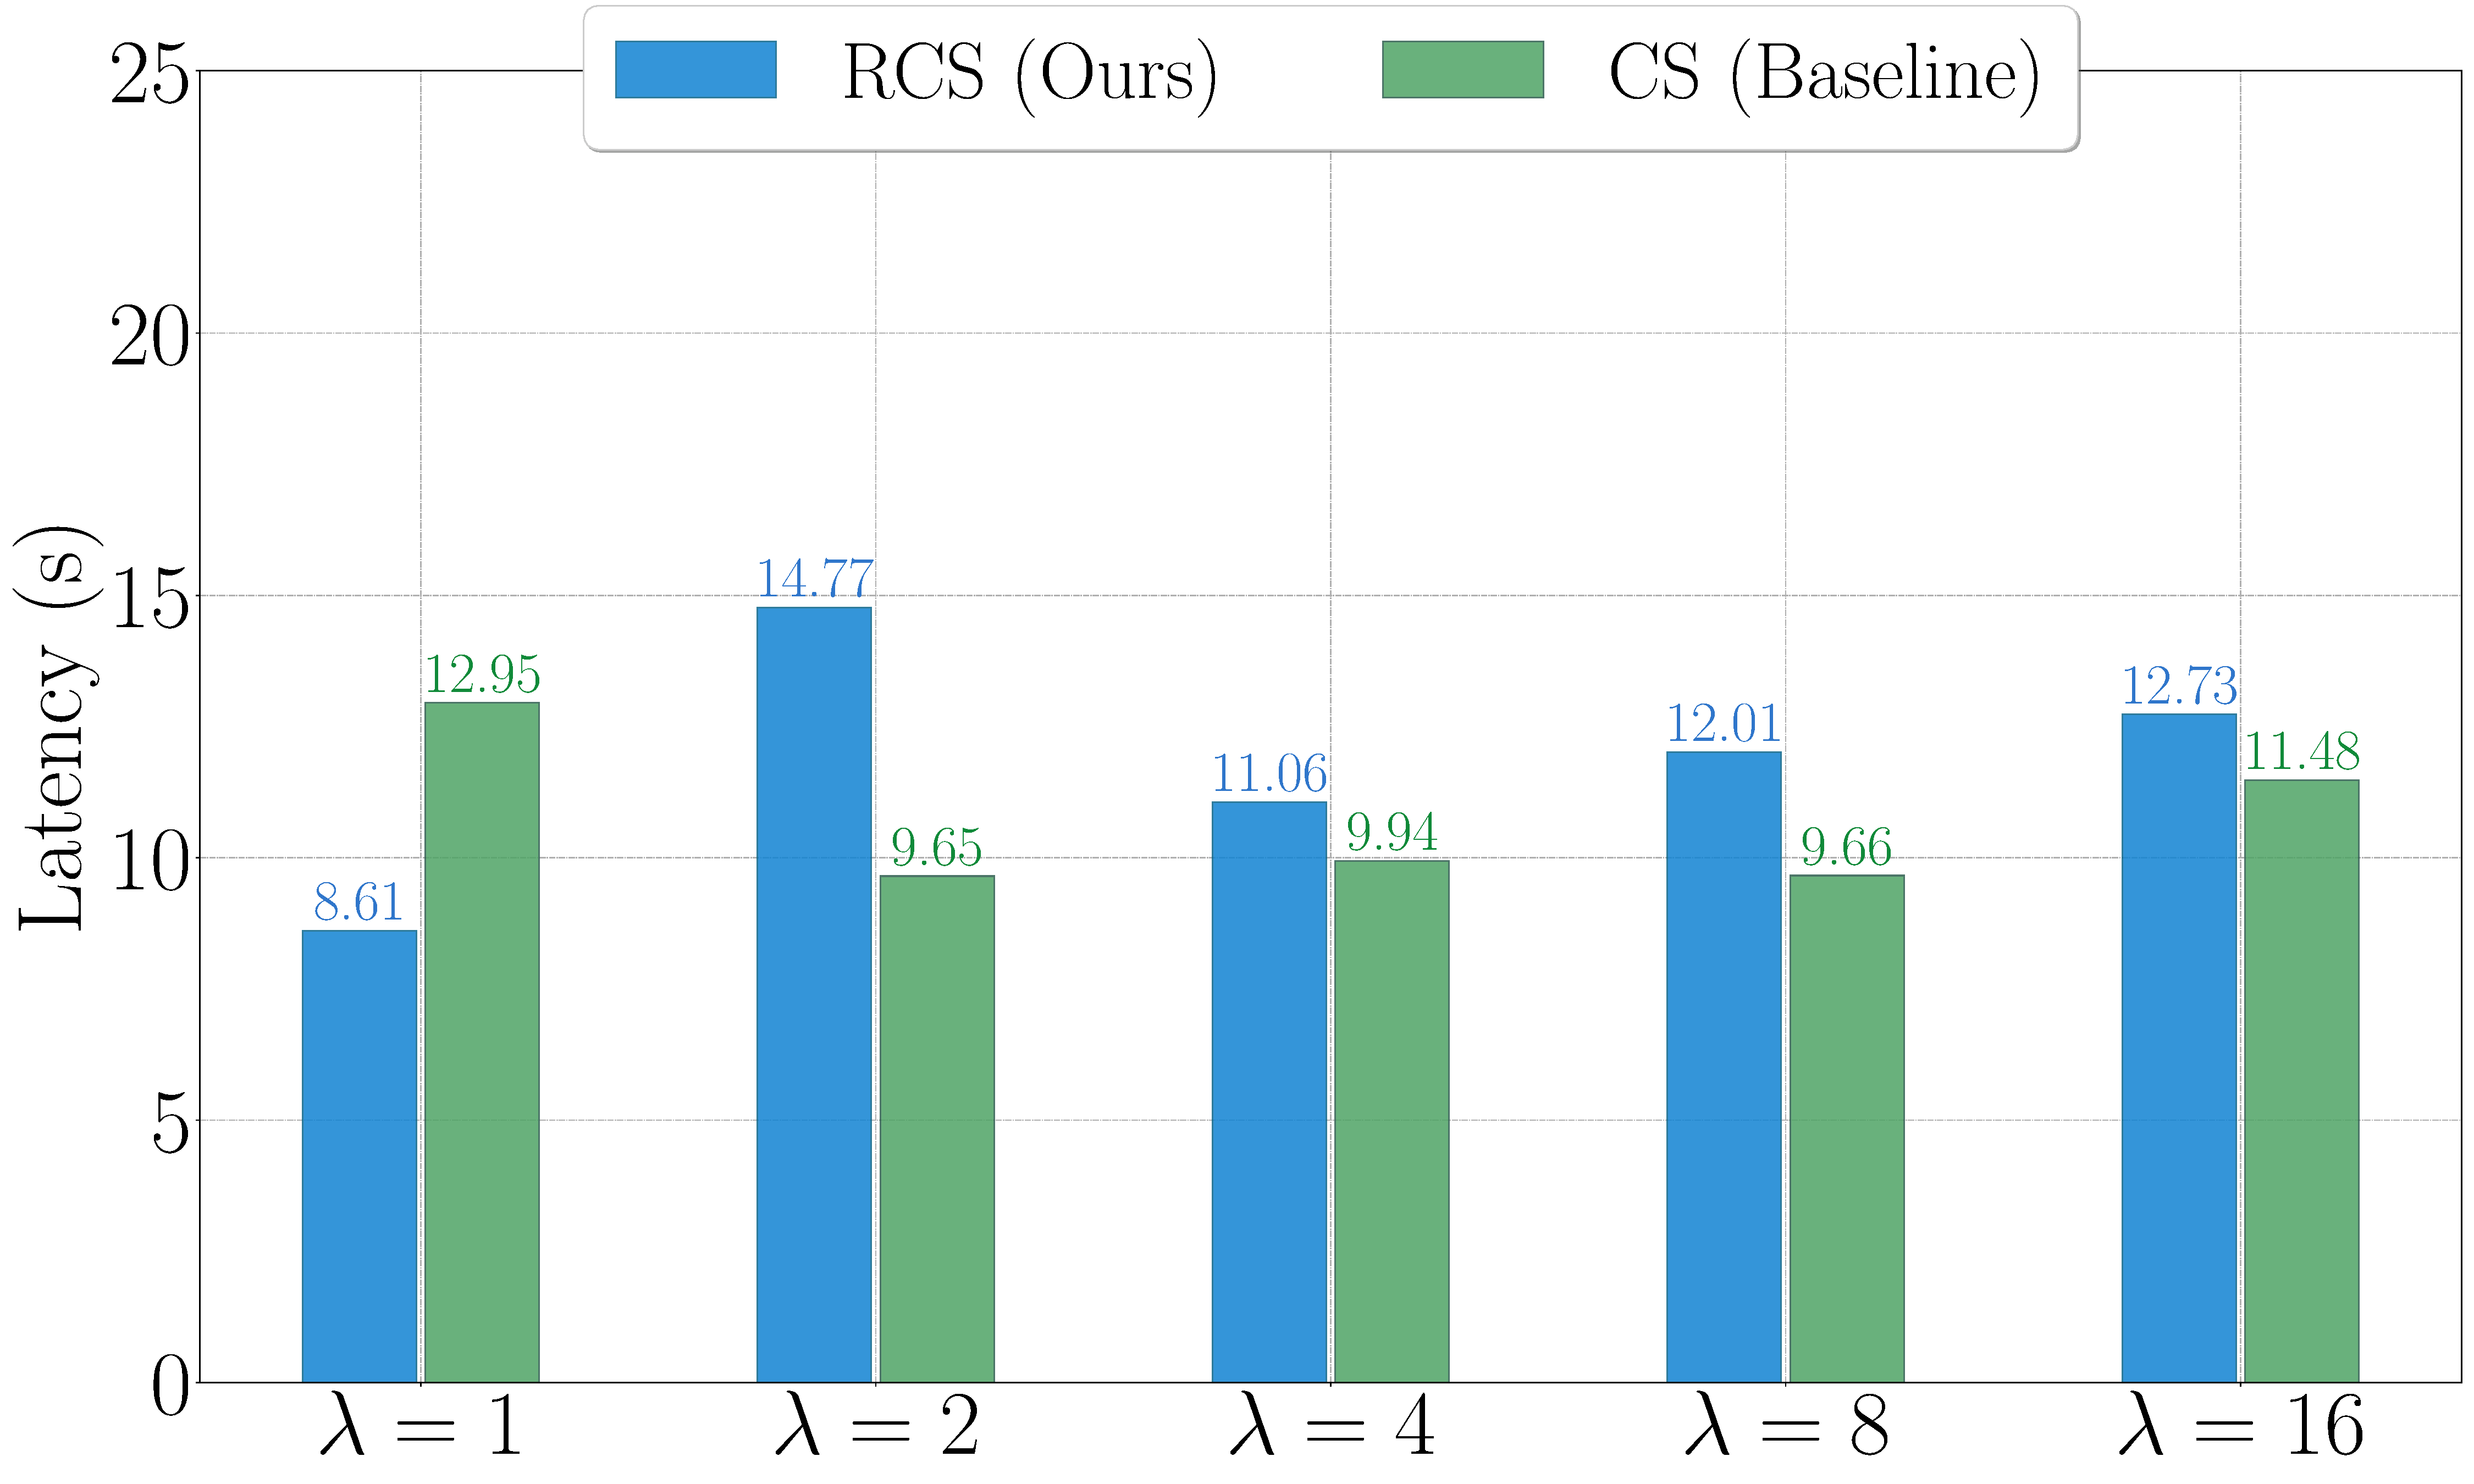
\includegraphics[width=\linewidth]{latex/eval_res/TC-33.pdf}
        \caption{$n=33$.}
    \end{subfigure}
    \begin{subfigure}{0.31\textwidth}
        \centering
        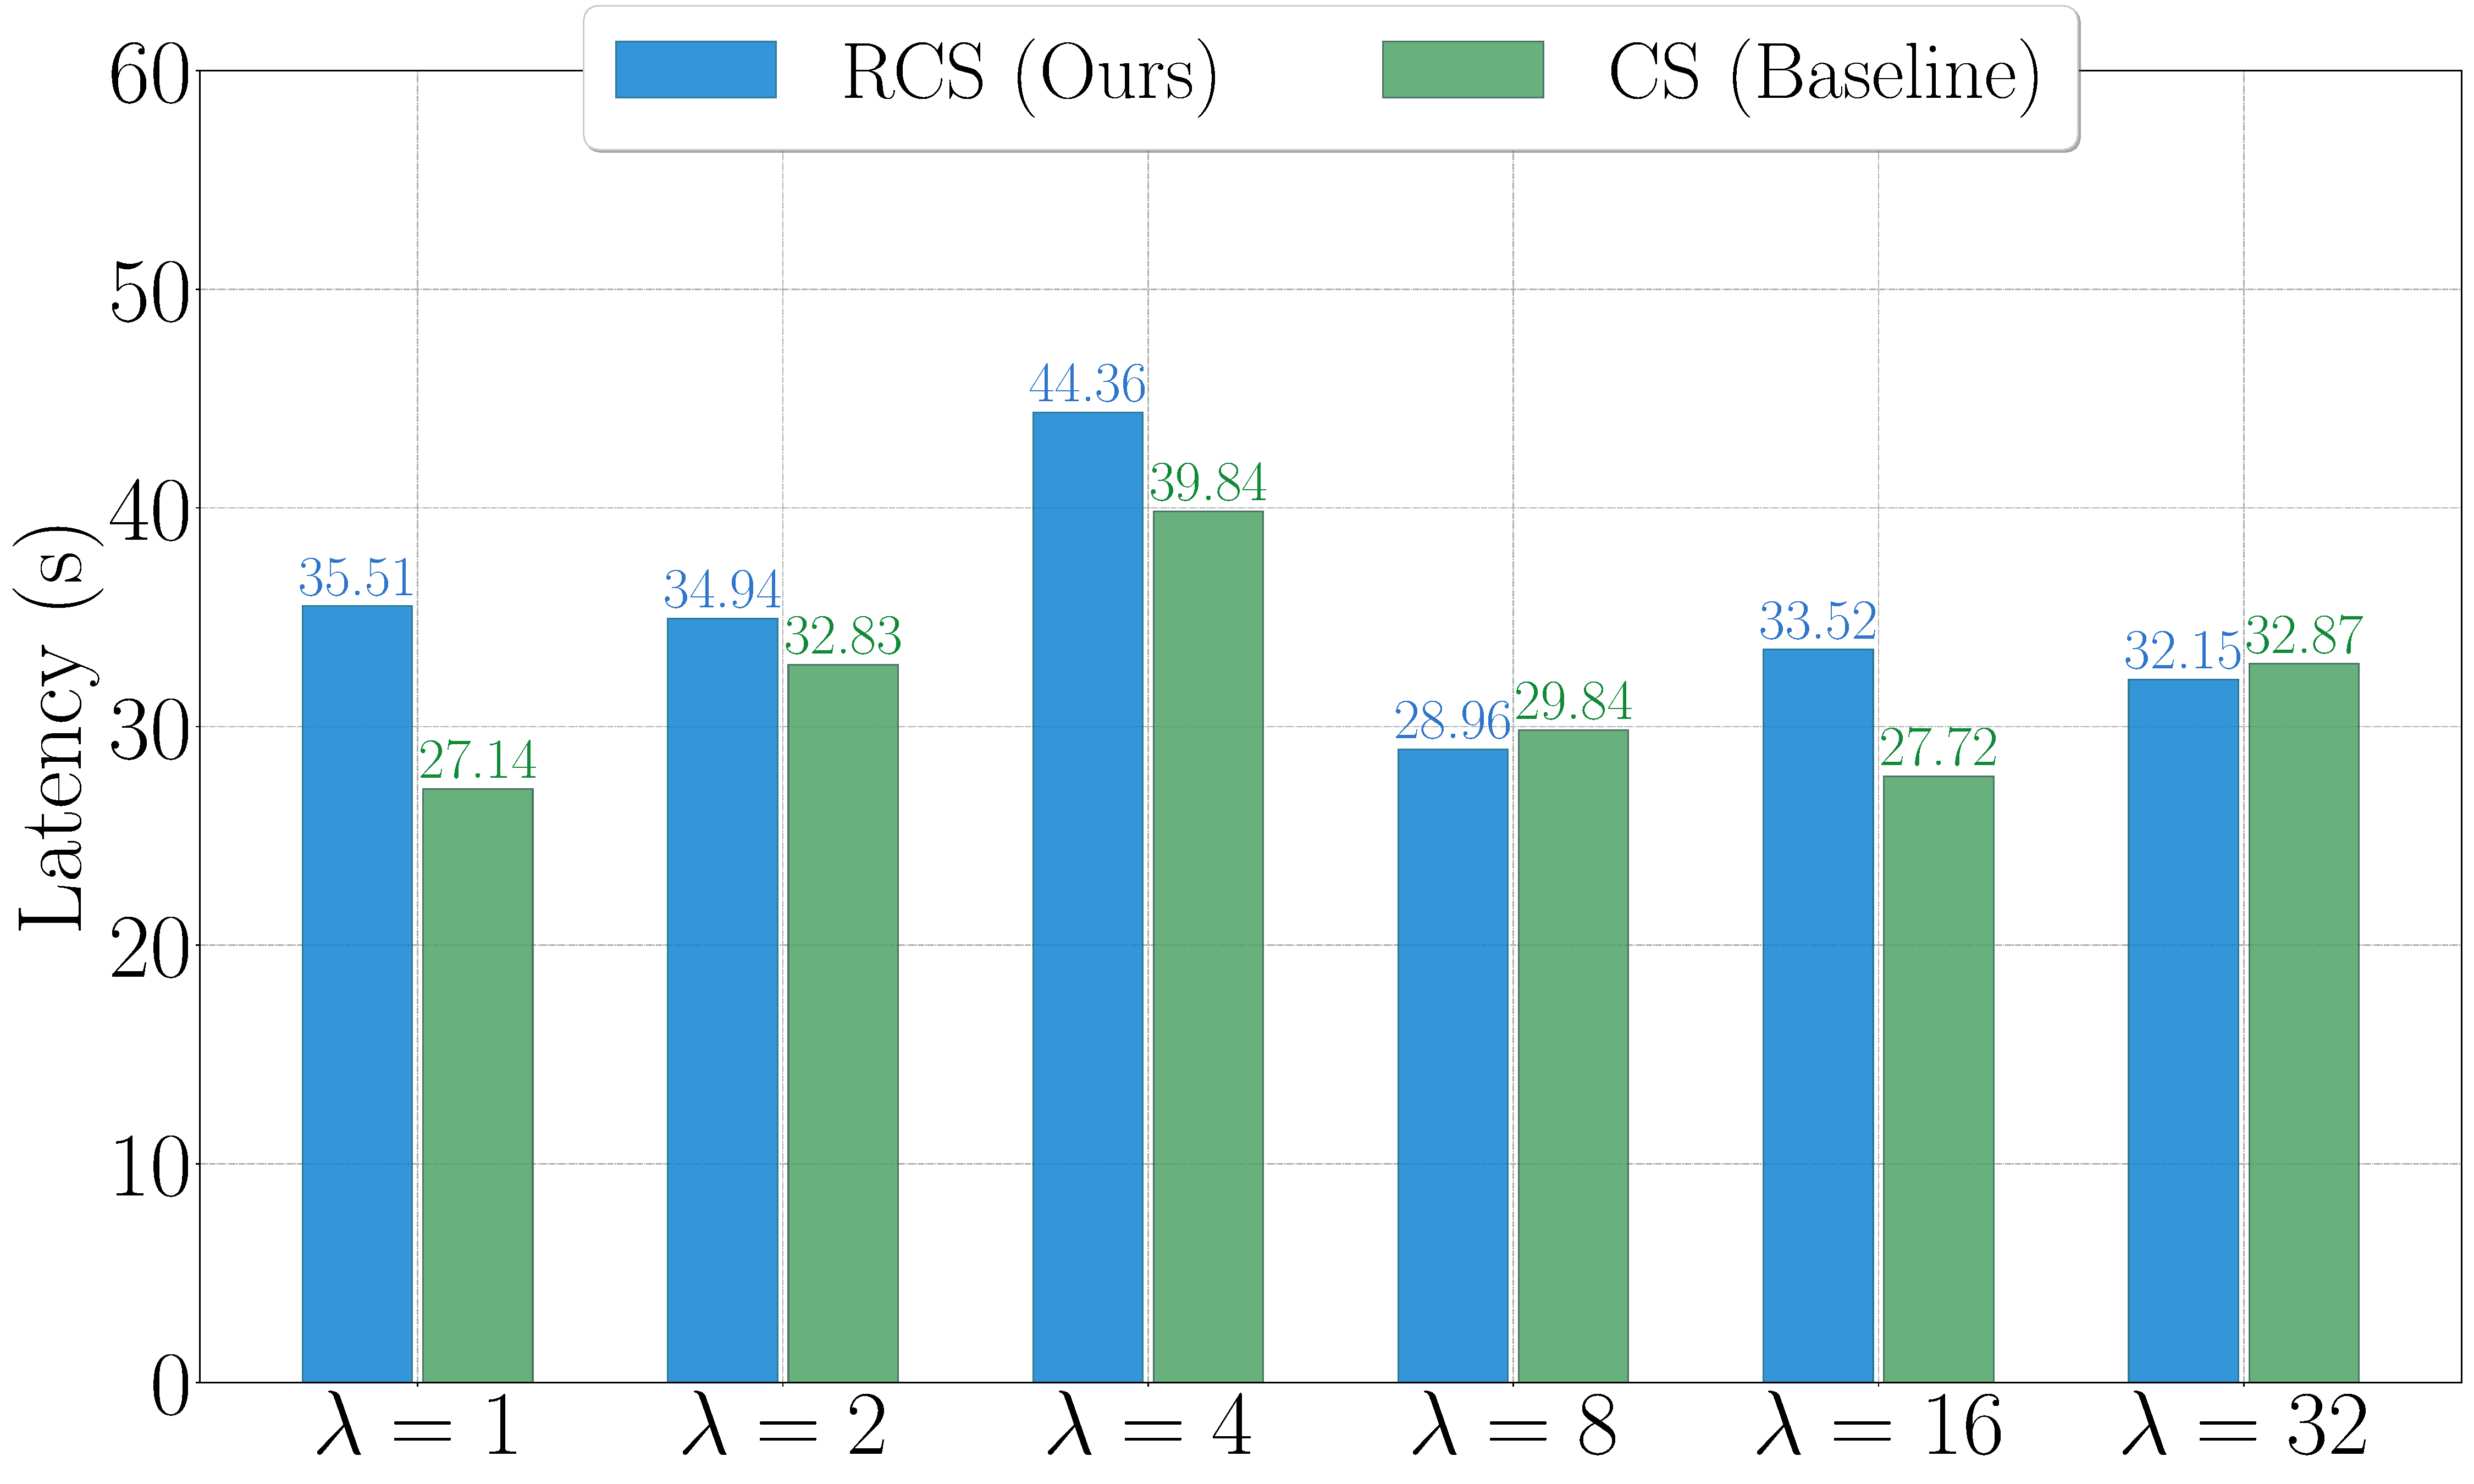
\includegraphics[width=\linewidth]{latex/eval_res/TC-65.pdf}
        \caption{$n=65$.}
    \end{subfigure}
    \begin{subfigure}{0.31\textwidth}
        \centering
        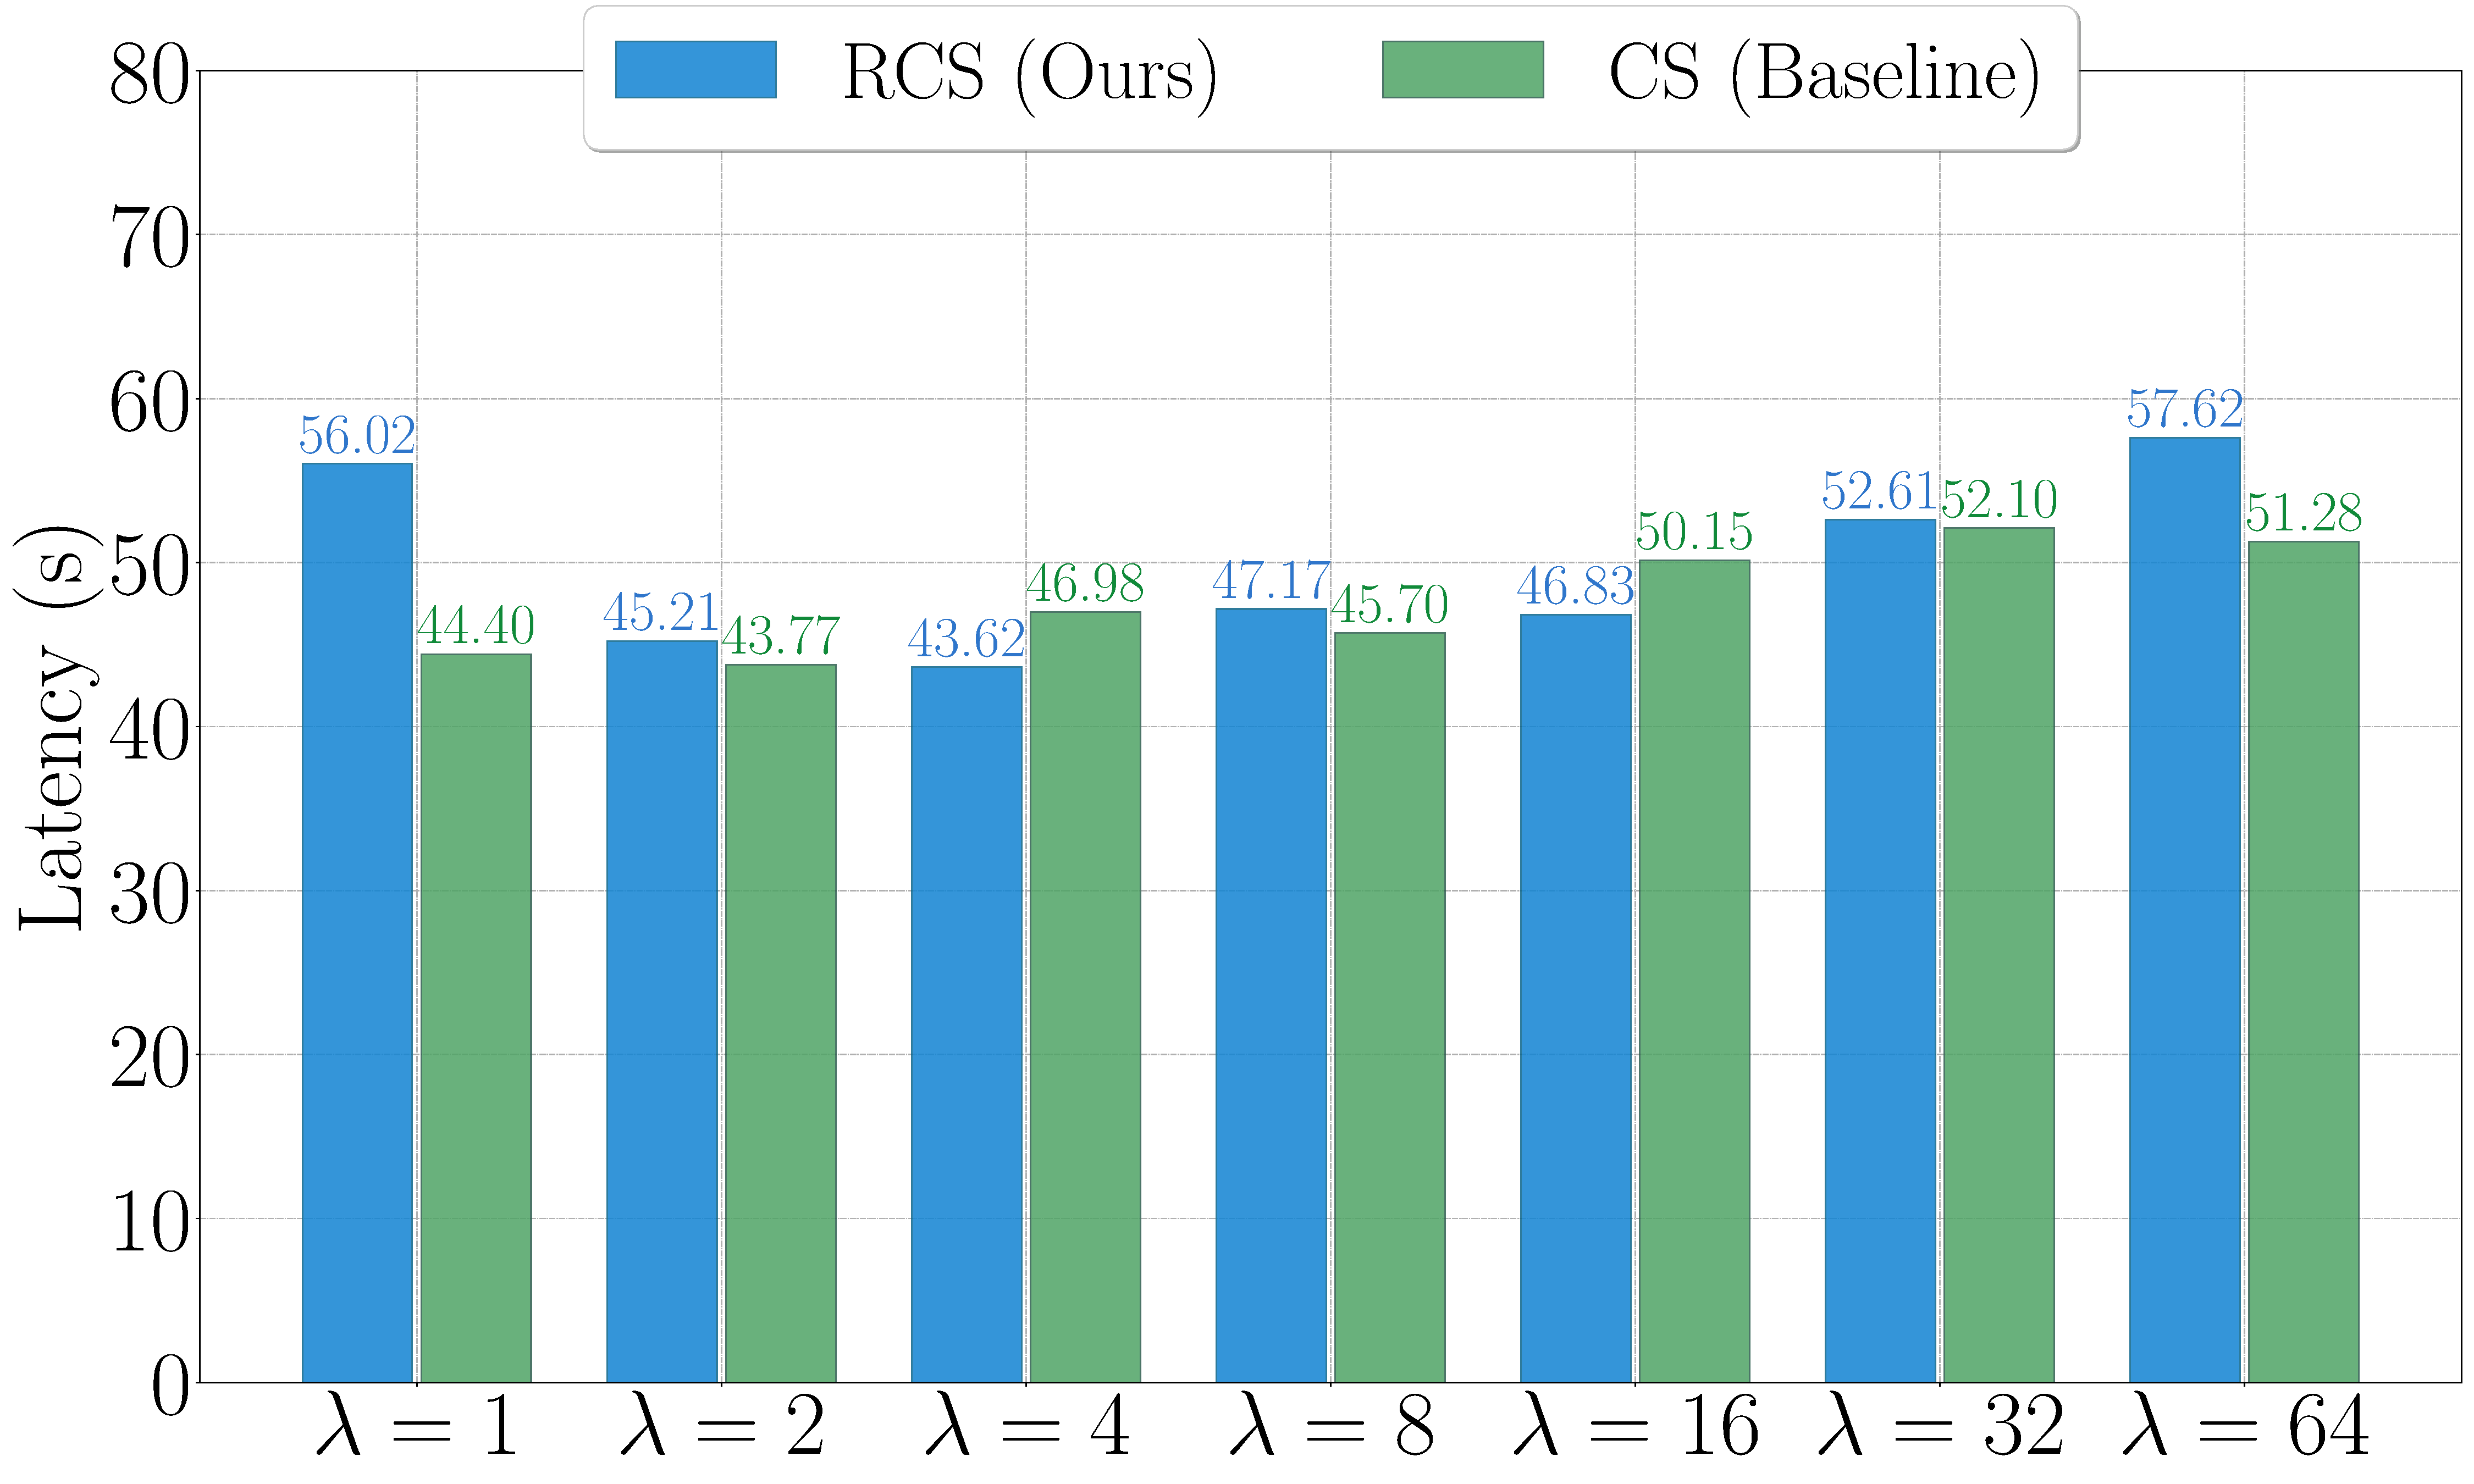
\includegraphics[width=\linewidth]{latex/eval_res/TC-129.pdf}
        \caption{$n=129$.}
    \end{subfigure}
    \caption{Evaluation results for the latency when $f < \lceil \frac{n}{2} \rceil$.}
    \label{fig:TC_g}
    % \vspace{-15pt}
\end{figure*}


\subsection{F-RCS Algorithm}
Based on the foundational theory in Section \ref{sec:Theory}, we construct an optimization algorithm for RCS, named Feedback-Optimized Reliable Consensus Sampling (F-RCS). In each sampling round, given the delivered response $y$ and the generating model $|\phi_r\rangle$, the algorithm identifies two additional models by a function $F(\cdot)$ (see Algorithm \ref{alg:F-RCS}). One model $|\phi_{\max}\rangle$ attains the maximum $p(y)$. Another model $|\phi_{\min}\rangle$ attains the minimum $p(y)$. If $y$ is judged unsafe at time $t$, then for subsequent similar tasks, $|\phi_{\max}\rangle$ is removed during random sampling. Formally, $\mathcal{MG} = \mathcal{MG} \setminus \{|\phi_{\max}\rangle\}.$ This allows, at the beginning of each algorithm execution, the system makes an automated decision. It selects safer models used in sampling for $x$. This process increases the safety margin $s - f$ and reduces risk. Here, $|\phi_{\max}\rangle$ can equal $|\phi_{r}\rangle$. Initially, $|\phi_{r}\rangle$ assigns the highest probability to $y$, which aligns with the algorithm objective. We call this behavior of model $|\phi_{r}\rangle$ self-entanglement. In addition, during sampling, the execution of the feedback algorithm is independent of RCS itself, and therefore does not affect the safety of RCS. For time overhead, the additional cost introduced by the feedback algorithm is negligible.



\begin{algorithm}[h]
\SetAlgoLined
\KwIn{
Parameters $(n, s, R)$;
evaluation method $a$
}
\KwOut{Response $y$}

\For{each prompt $x$}{
    $|\phi_{r}\rangle \gets F(x, \mathcal{MG})$ \\
    $\mathcal{MG}^{'} \gets \mathcal{MG} \setminus \{|\phi_{r}\rangle\}$ \\
    $\{y,\mathcal{P}\} \gets \text{RCS}(\mathcal{MG}^{'}, x, s, R)$ \\
    \textcolor{mGreen}{\#$\mathcal{P}=\{p_{|\phi_1\rangle}(y), \cdots, p_{|\phi_n\rangle}(y) \}$} \\
    \textcolor{mGreen}{\#Identify entangled models.} \\
    $|\phi_{\max}\rangle \gets \arg\max_{|\phi_i\rangle} p_{|\phi_i\rangle}(y)$ \\
    \textcolor{mGreen}{\#Record $<|\phi_{\max}\rangle\ ,x, y, |\phi_{r}\rangle>$.} \\
    \Return $y$ \\
    }
    
\While{time $t \in \mathbb{R}^{+}$}{
    \If{$|1\rangle \gets \mathrm{Eval}(x, |\phi_{r}\rangle, a)$}{
        New $F \gets \mathrm{Update}(F,|\phi_{\max}\rangle\ ,x)$ \\
    }
    $t \gets t + \Delta(t)$\\
}

\caption{F-RCS Algorithm}
\label{alg:F-RCS}
\end{algorithm}




\section{Experiments}
\label{sec:experiment}
Although Section \ref{sec:Methodology} presents a theoretical analysis that validates the advantages and effectiveness of our method, we still conduct extensive experiments to demonstrate its practical performance.



\subsection{Experimental Setup}
\noindent
\textbf{Parameter Settings}.
We follow the cryptography \citep{Ruan2025haw, Couteau2022sharp} for selecting the security parameter $\lambda$ and set
$\lambda = 2^d, d \in \mathbb{Z}.$ We choose $R = \lambda + 1$. The values of $s$ and $f$ are determined according to specific types of experiments, and we set $n = kR + b$. From a practical perspective, the relationship between $s$ and $n$ is unknown. The value of $s$ needs to be specified when deploying the algorithm. $s$ does not reflect the actual number of safe models in the $\mathcal{MG}$. To cover general practical scenarios, we adopt the weakest security assumption and set $s = \lceil \frac{n+1}{2} \rceil$. This setting is similar to the widely used $3f+1=n$ in distributed systems research \citep{zhang2023waterbear, Zhang2022pace}.



\noindent
\textbf{Datasets and Models}. 
To reflect adversarial conditions in real-world scenarios, we construct the probability distribution of the safe model using the output distributions of Qwen2.5-7b-instruct, Qwen2.5-0.5b-instruct \citep{qwen2025qwen25technicalreport}, and Qwen3Guard-Gen-8B \citep{zhao2025qwen3guard} on safety evaluation datasets. The datasets include HarmBench \citep{mazeika2024harmbench} and AdvBench \citep{zou2023universal}. We generate the perturbed probability distributions of the unsafe models by referring to the probability distribution of the safe model. This process simulates $f$ Byzantine models that an adversary can fully control. 

\noindent
\textbf{Evaluation Protocol}. To reduce randomness, we report experimental results obtained from 8,000 repeated experiments.



\begin{figure*}[!]
    \centering
    \begin{subfigure}{0.32\textwidth}
        \centering
        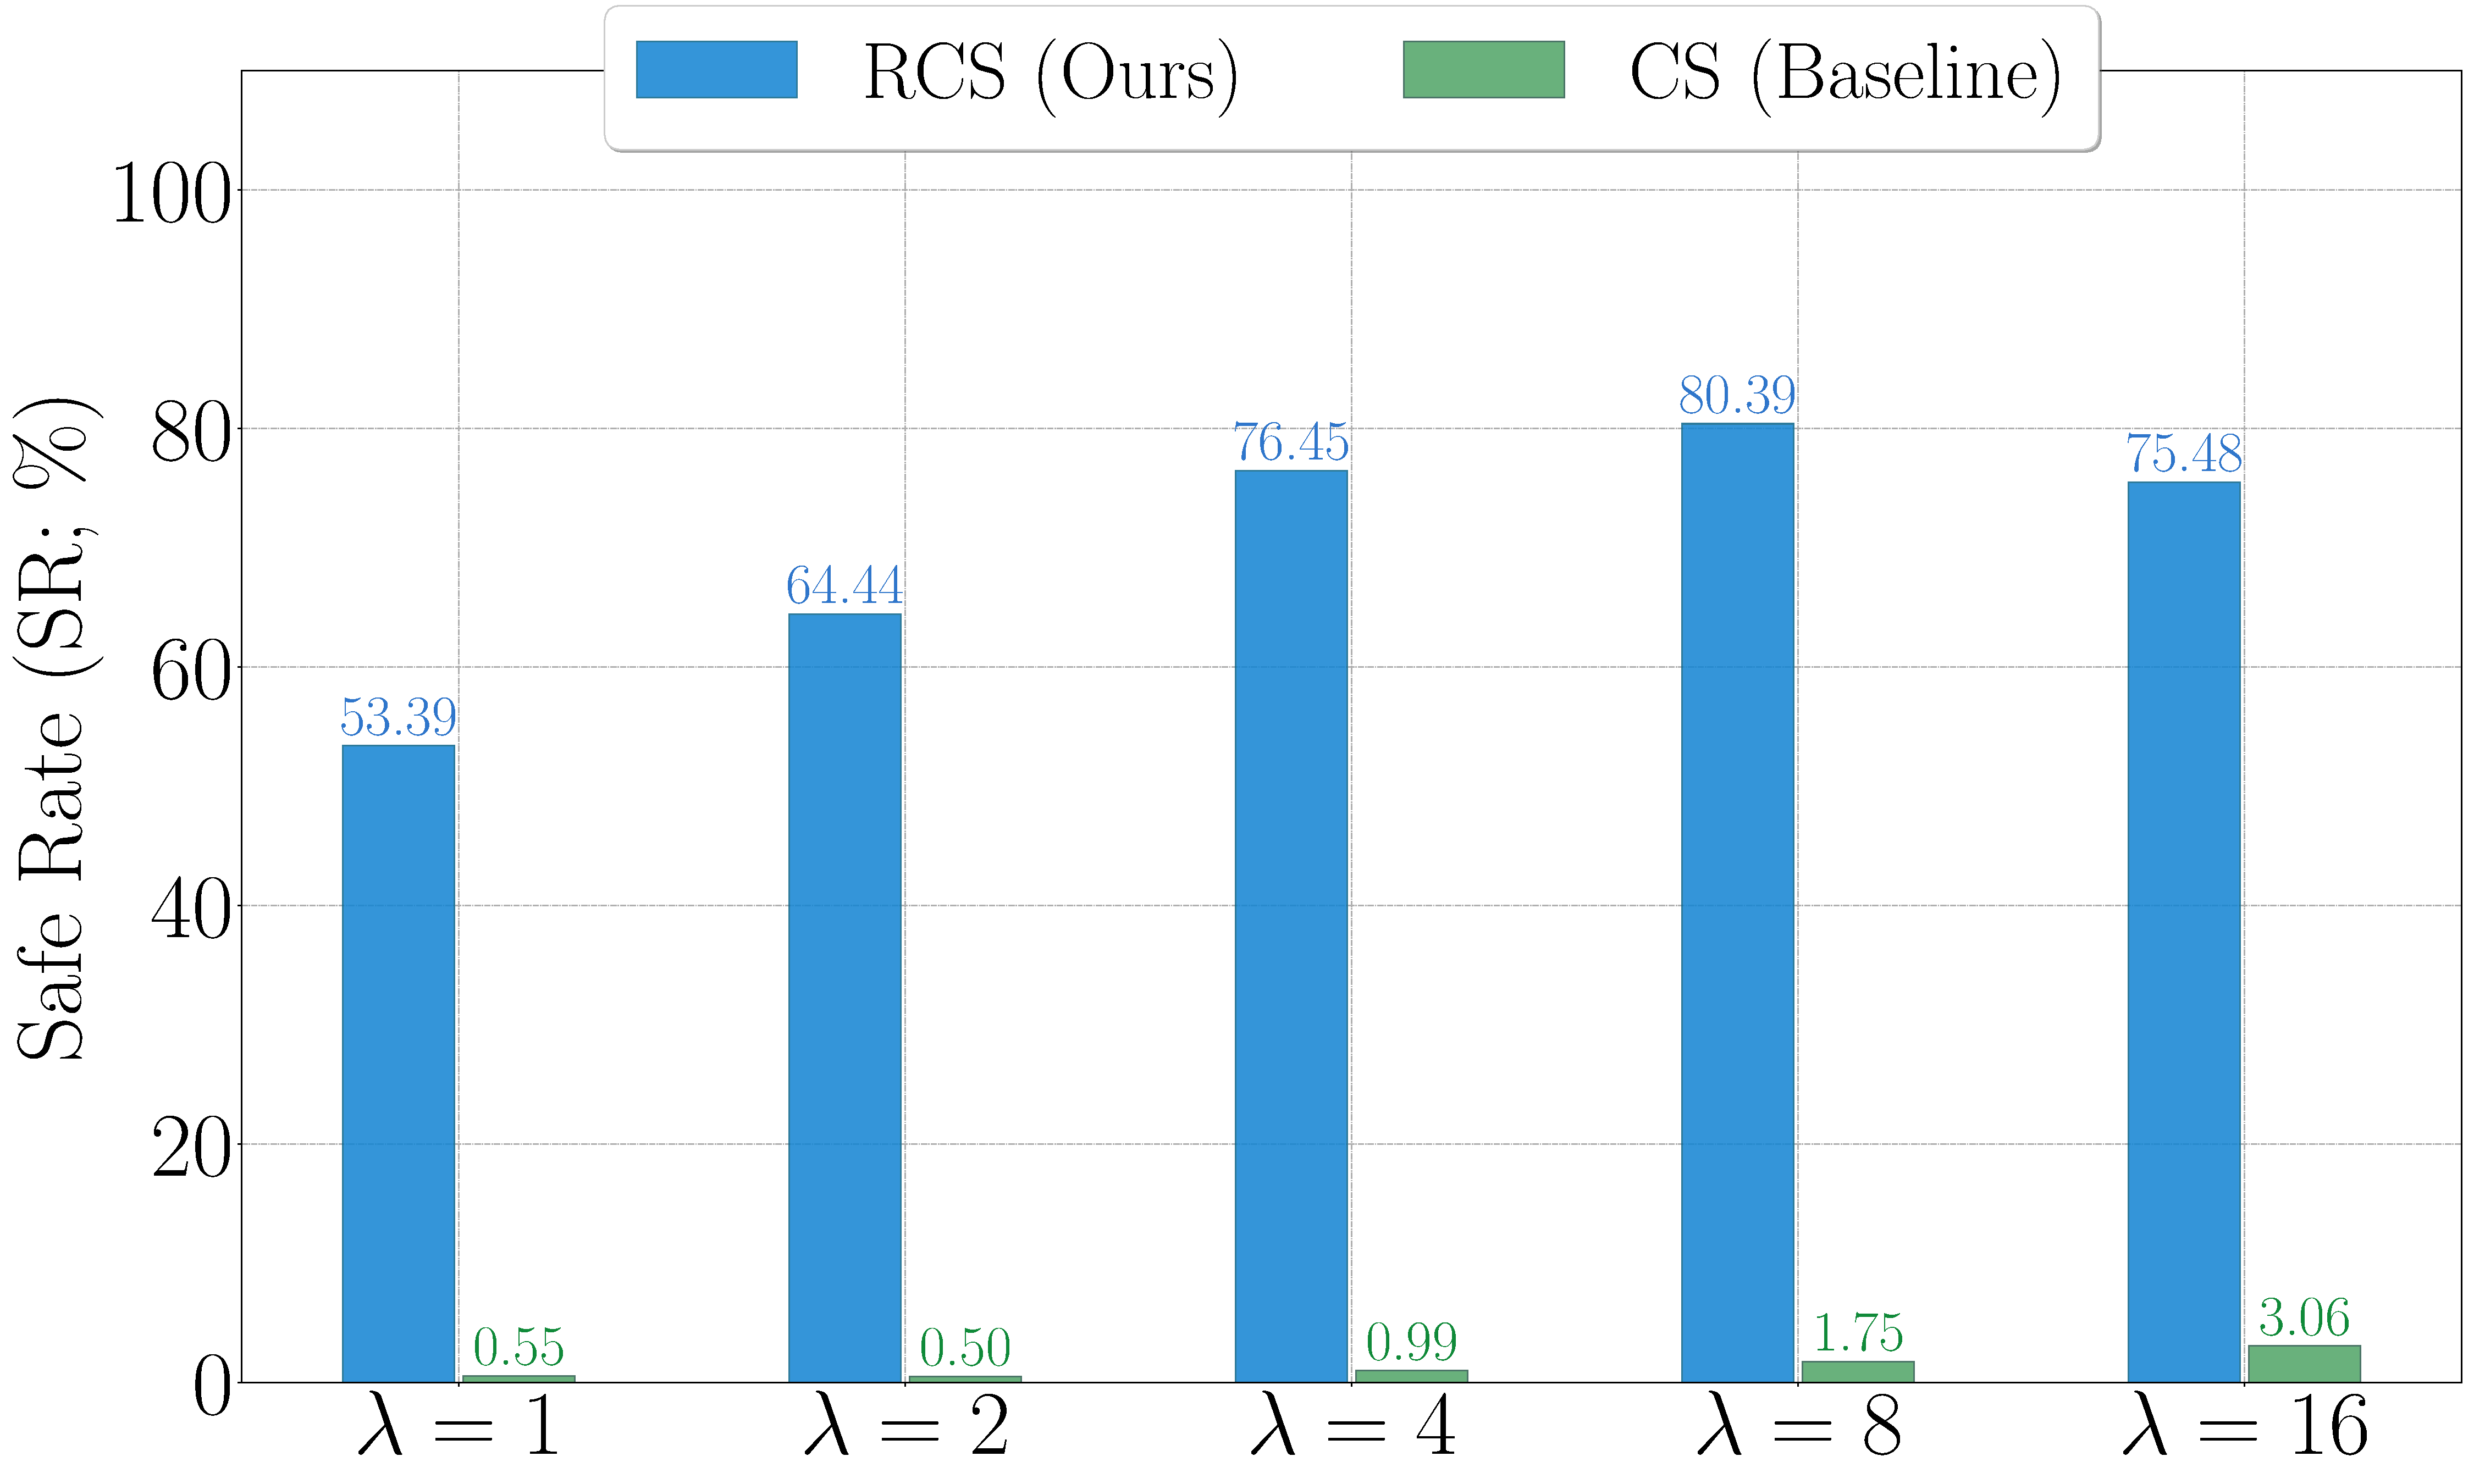
\includegraphics[width=\linewidth]{latex/eval_res_m/SR-33-m.pdf}
        \caption{$n=33$.}
    \end{subfigure}
    \begin{subfigure}{0.32\textwidth}
        \centering
        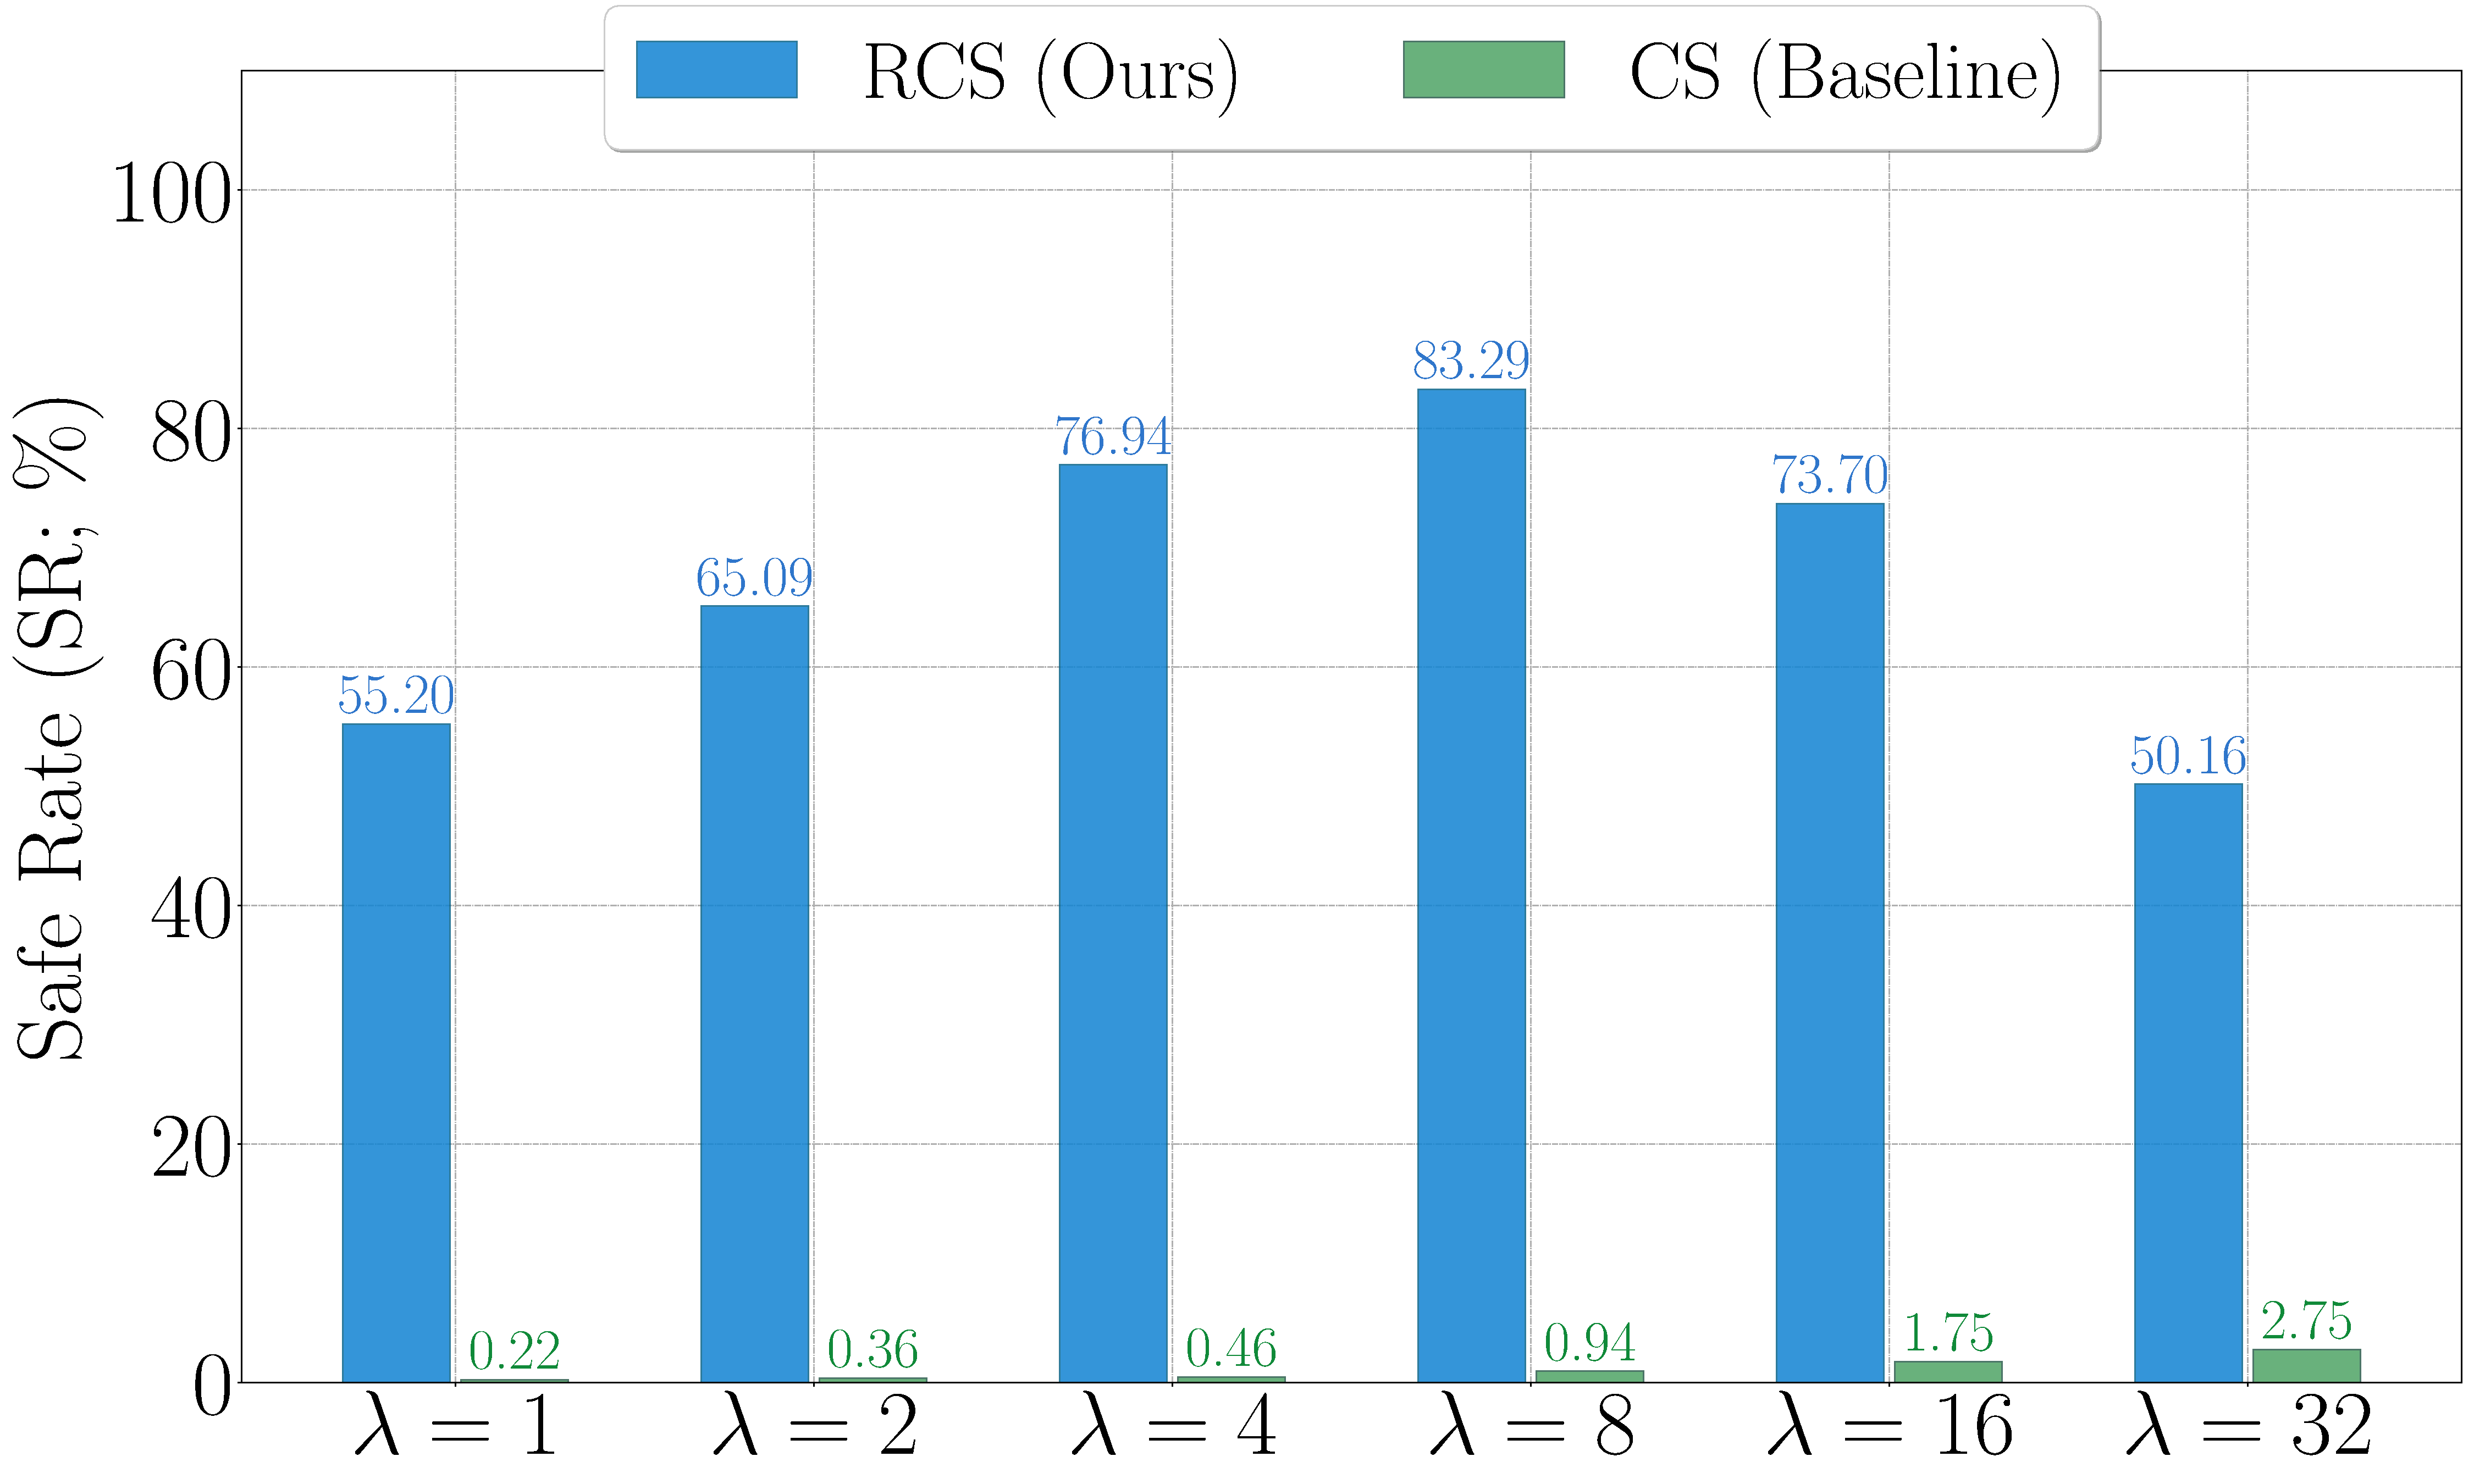
\includegraphics[width=\linewidth]{latex/eval_res_m/SR-65-m.pdf}
        \caption{$n=65$.}
    \end{subfigure}
    \begin{subfigure}{0.32\textwidth}
        \centering
        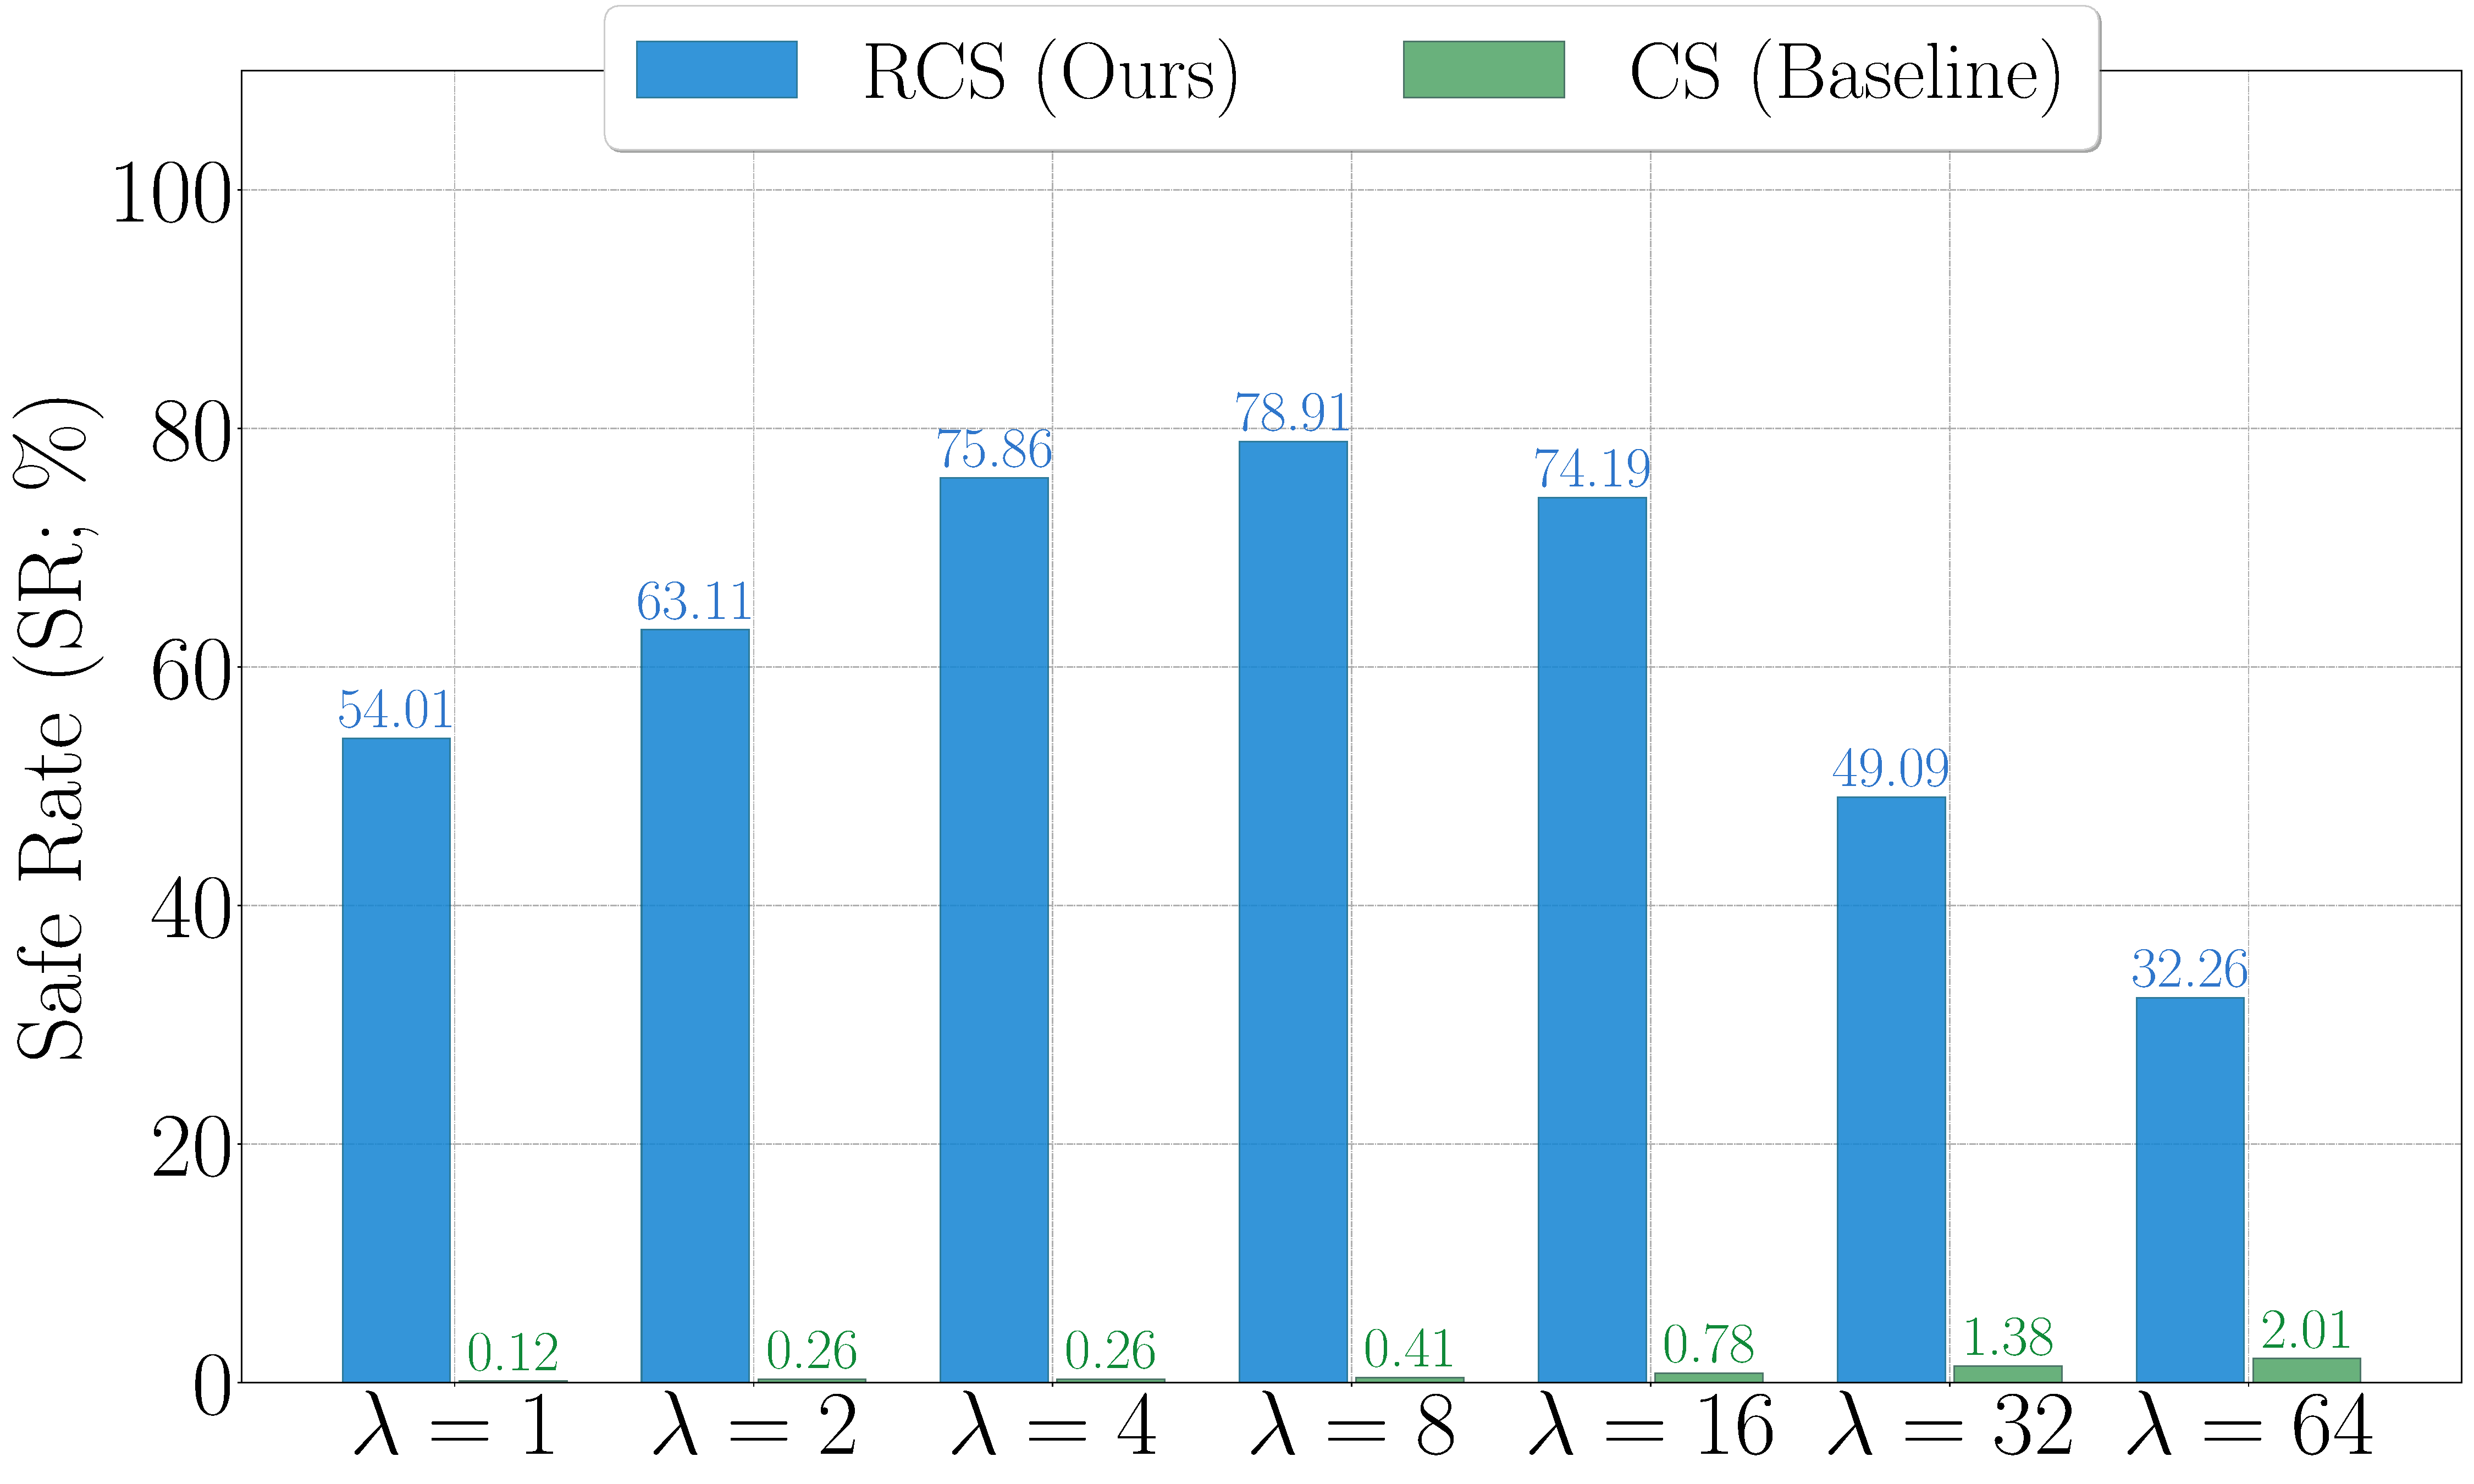
\includegraphics[width=\linewidth]{latex/eval_res_m/SR-129-m.pdf}
        \caption{$n=129$.}
    \end{subfigure}
    \caption{Evaluation results for the safe rate when Byzantine models collude.}
    \label{fig:SR_m}
    \vspace{-5pt}
\end{figure*}






\begin{figure*}[!]
    \centering
    \begin{subfigure}{0.32\textwidth}
        \centering
        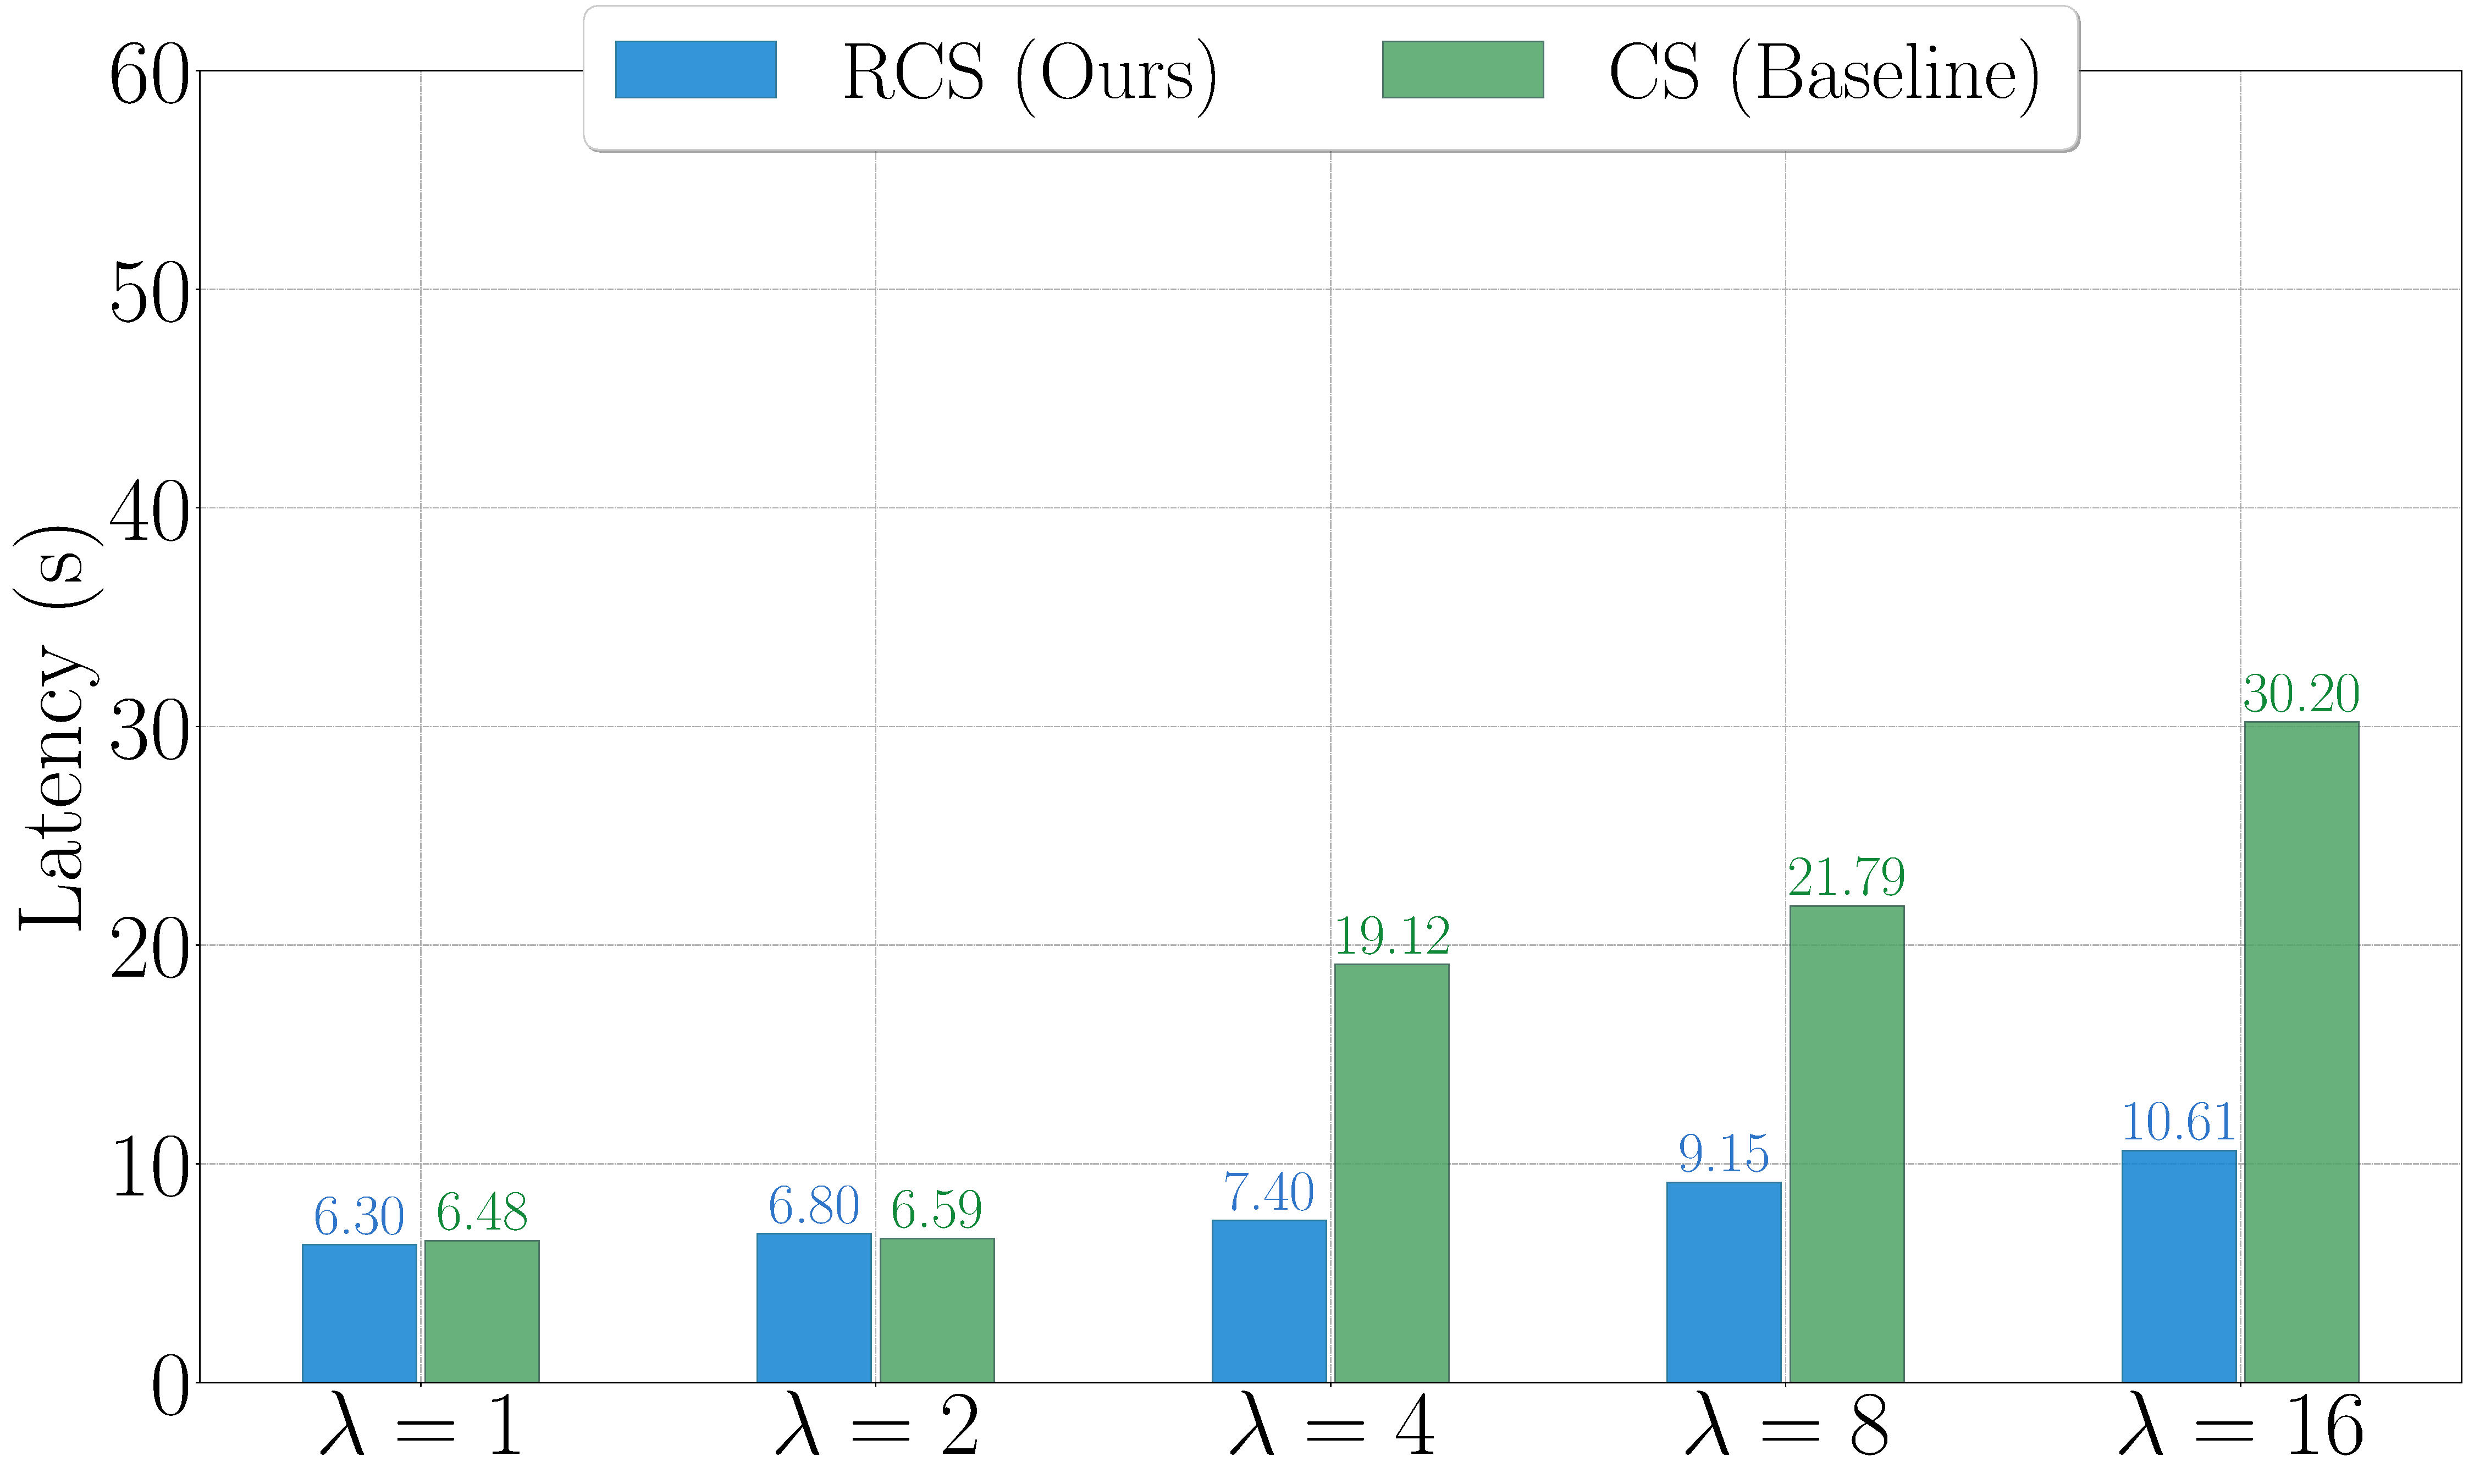
\includegraphics[width=\linewidth]{latex/eval_res_m/TC-33-m.pdf}
        \caption{$n=33$.}
    \end{subfigure}
    \begin{subfigure}{0.32\textwidth}
        \centering
        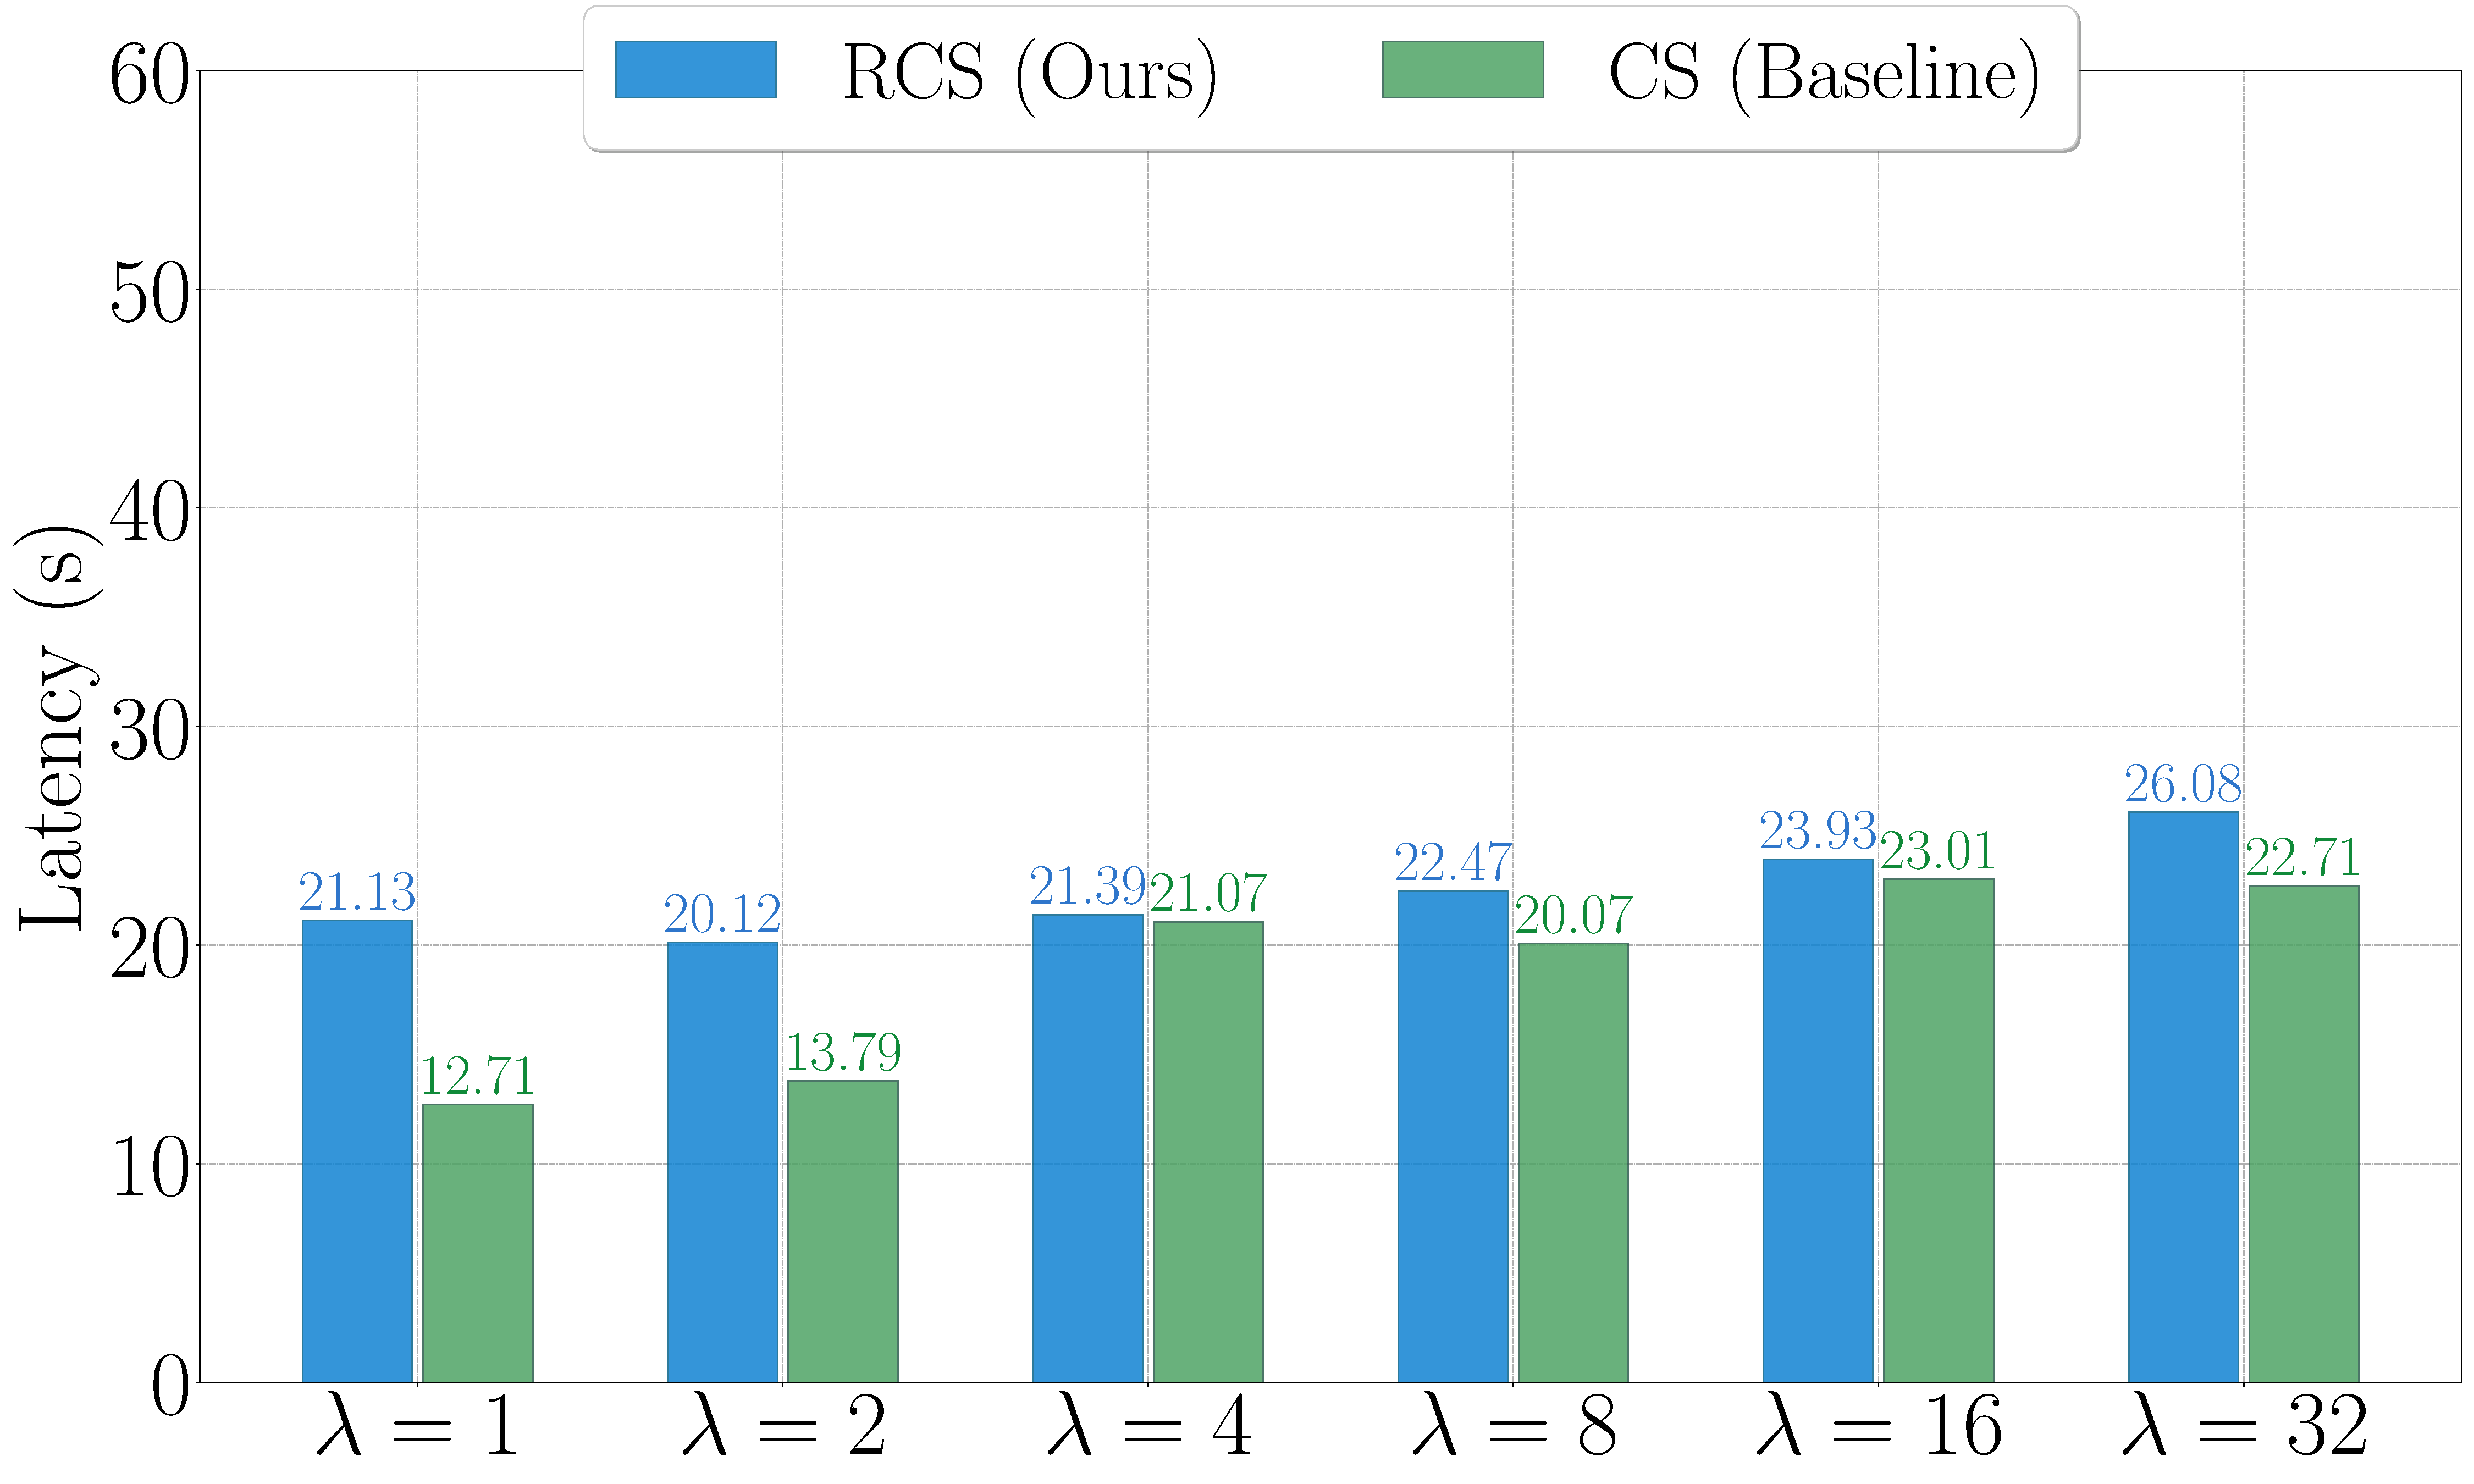
\includegraphics[width=\linewidth]{latex/eval_res_m/TC-65-m.pdf}
        \caption{$n=65$.}
    \end{subfigure}
    \begin{subfigure}{0.32\textwidth}
        \centering
        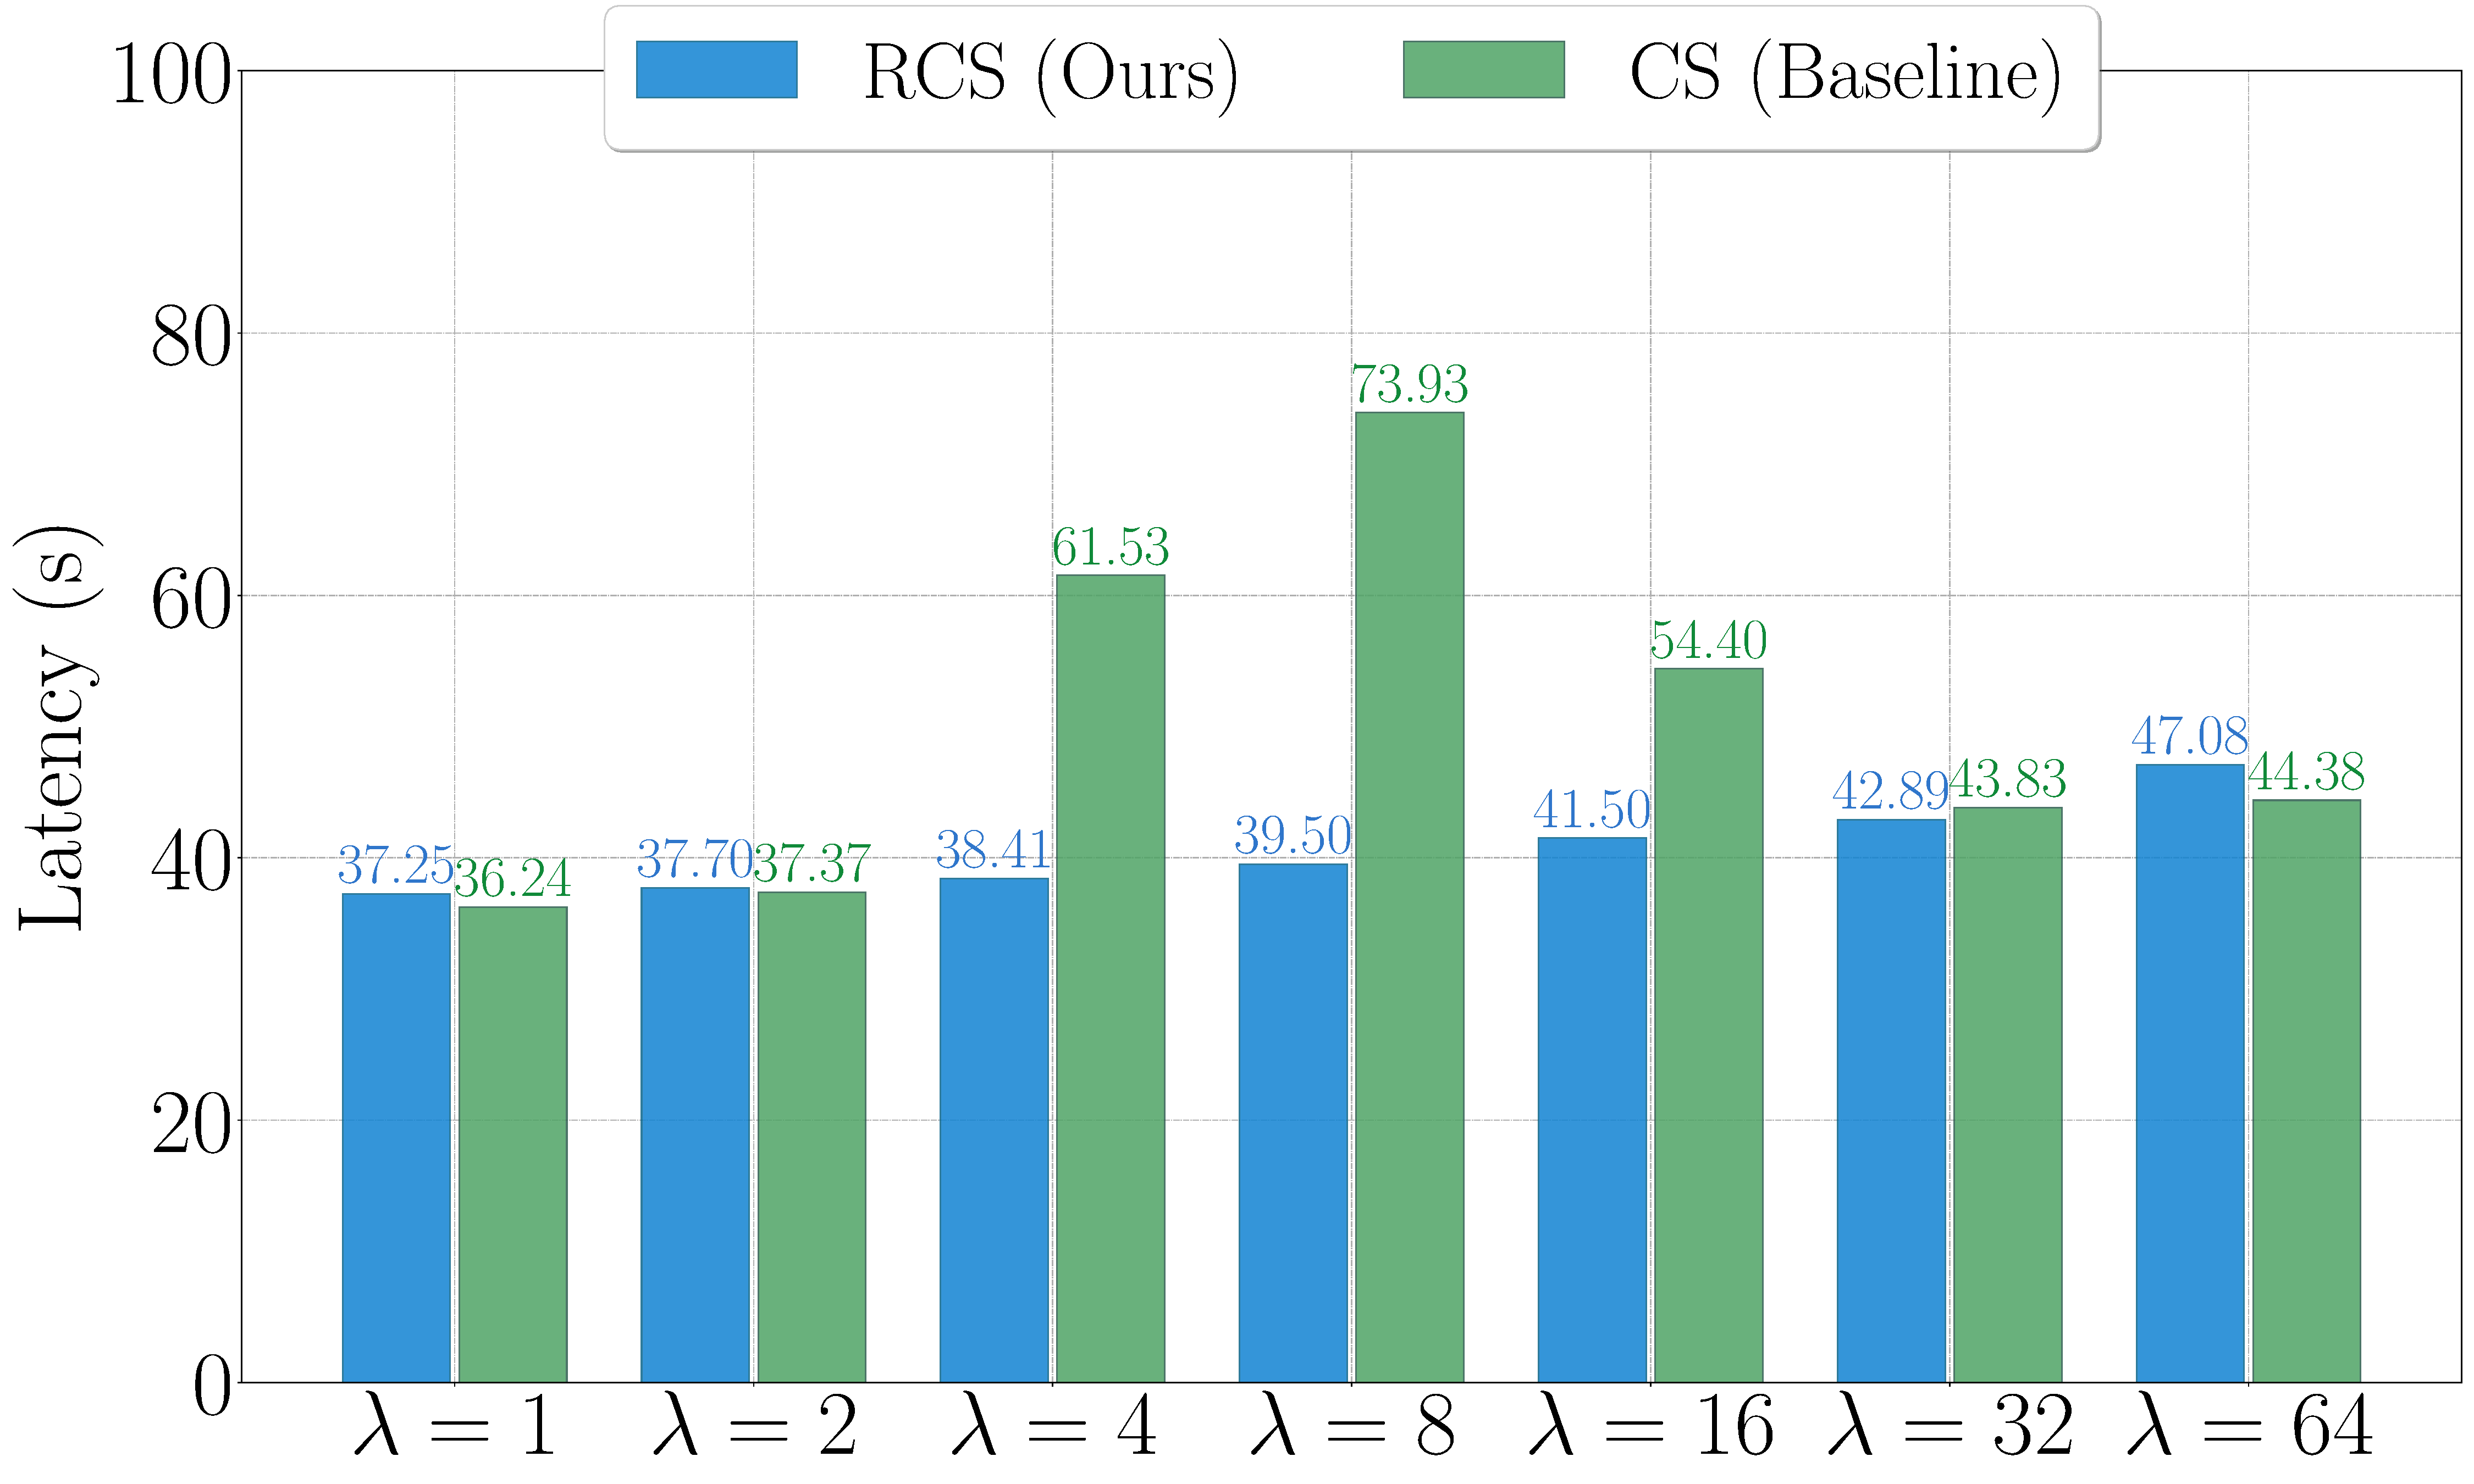
\includegraphics[width=\linewidth]{latex/eval_res_m/TC-129-m.pdf}
        \caption{$n=129$.}
    \end{subfigure}
    \caption{Evaluation results for the latency when Byzantine models collude.}
    \label{fig:TC_m}
    \vspace{-15pt}
\end{figure*}





\subsection{Evaluation Metrics}
In this work, we do not define specific criteria that label a response as safe or unsafe. For example, under jailbreak attacks, LLMs may output tokens such as "Sorry" or "Sure" \citep{wang-etal-2025-vulnerability}. These outputs reflect temporary experimental observations. They do not imply provable security in a theoretical sense. Therefore, our evaluation does not rely on the LLM-as-a-judge \citep{wei2025emoji} commonly used in prior jailbreak studies. We define the evaluation metrics as follows. Safe rate (SR) denotes the proportion of final responses produced by the safe models. Abstention rate (AR) denotes the proportion of cases where the $\mathcal{MG}$ returns $\perp$ instead of a usable response. Latency denotes the time interval from the start of the sampling to the delivery of the final response. Accuracy measures the precision of the feedback algorithm in F-RCS when identifying unsafe models, that is, the proportion of models detected by the feedback algorithm that are indeed unsafe.

\subsection{Experimental Results}
We evaluate settings where $f < \lceil \frac{n}{2} \rceil$. The results for large values of $n$ are shown in \autoref{fig:SR_g} and \autoref{fig:TC_g}. Results for smaller values of $n$ are reported in \autoref{app:results}. For different values of the security parameter $\lambda$, RCS achieves significantly higher safety than CS. RCS maintains comparable overall latency to CS. These results are consistent with the theoretical analysis and proofs in Section \ref{sec:Methodology}. CS often leads to abstention, which reduces SR. We further evaluate the algorithms under Byzantine model collusion. Results for large values of $n$ are shown in \autoref{fig:SR_m} and \autoref{fig:TC_m}. Under collusion, the safety of CS degrades catastrophically compared to the $f < \lceil \frac{n}{2} \rceil$ setting. In contrast, the safety of RCS is only slightly affected. RCS maintains more than $67\%$ safety. This result demonstrates strong resistance to collusion. To assess half-resilience, we also evaluate the case where $f = \lceil \frac{n}{2} \rceil$. The results are reported in \autoref{app:results}. In this case, CS again exhibits clear safety weaknesses and performs significantly worse than RCS. \autoref{tab:comparison} reports aggregated results across all values of $\lambda$ and $n$. RCS outperforms CS in both SR and AR. RCS also achieves comparable latency to CS. These results further validate the theoretical analysis and proofs.

For F-RCS, we evaluate the accuracy of the feedback algorithm in identifying unsafe models. The results are shown in \autoref{fig:dr} and \autoref{app:results}. We show that for different values of $\lambda$ and $n$, the average accuracy remains around 90\%. This result demonstrates the effectiveness of the feedback algorithm.



\begin{table*}[t]
\centering
\scalebox{0.87}{
    \setlength{\tabcolsep}{6pt}
    \begin{tabular}{l|llll|llll}
    \toprule
    \multirow{2}{*}{\textbf{Method}} 
    & \multicolumn{4}{c|}{\textbf{Consensus Sampling (Baseline)}} 
    & \multicolumn{4}{c}{\textbf{Reliable Consensus Sampling (Ours)}} \\
    \cmidrule(lr){2-5} \cmidrule(lr){6-9}
    & $f < \lceil \frac{n}{2} \rceil$ & $f = \lceil \frac{n}{2} \rceil$ & Collusion & AVG & $f < \lceil \frac{n}{2} \rceil$ & $f = \lceil \frac{n}{2} \rceil$ & Collusion & AVG \\
    \midrule
    Safe Rate       & 20.39 & 15.83 & 1.45  & 12.56 & 82.88 & 81.49 & 67.90 & \textbf{77.42} ($\uparrow\times 5.16$) \\
    Abstention Rate & 71.79 & 72.52 & 82.95 & 75.75 & 0.00  & 0.00 & 0.00 & \textbf{0.00} ($\downarrow 100\%$) \\
    Latency         & 22.60 & 26.73 & 21.43 & 23.59 & 24.26 & 22.21 & 18.42 & \textbf{21.63} ($\downarrow 8.31\%$) \\
    \bottomrule
    \end{tabular}
}
\caption{Comprehensive comparison between our RCS and the baseline across different dimensions. Boldface indicates the best value in each dimension.}
\label{tab:comparison}
\vspace{-10pt}
\end{table*}


\begin{figure}[t]
    \centering
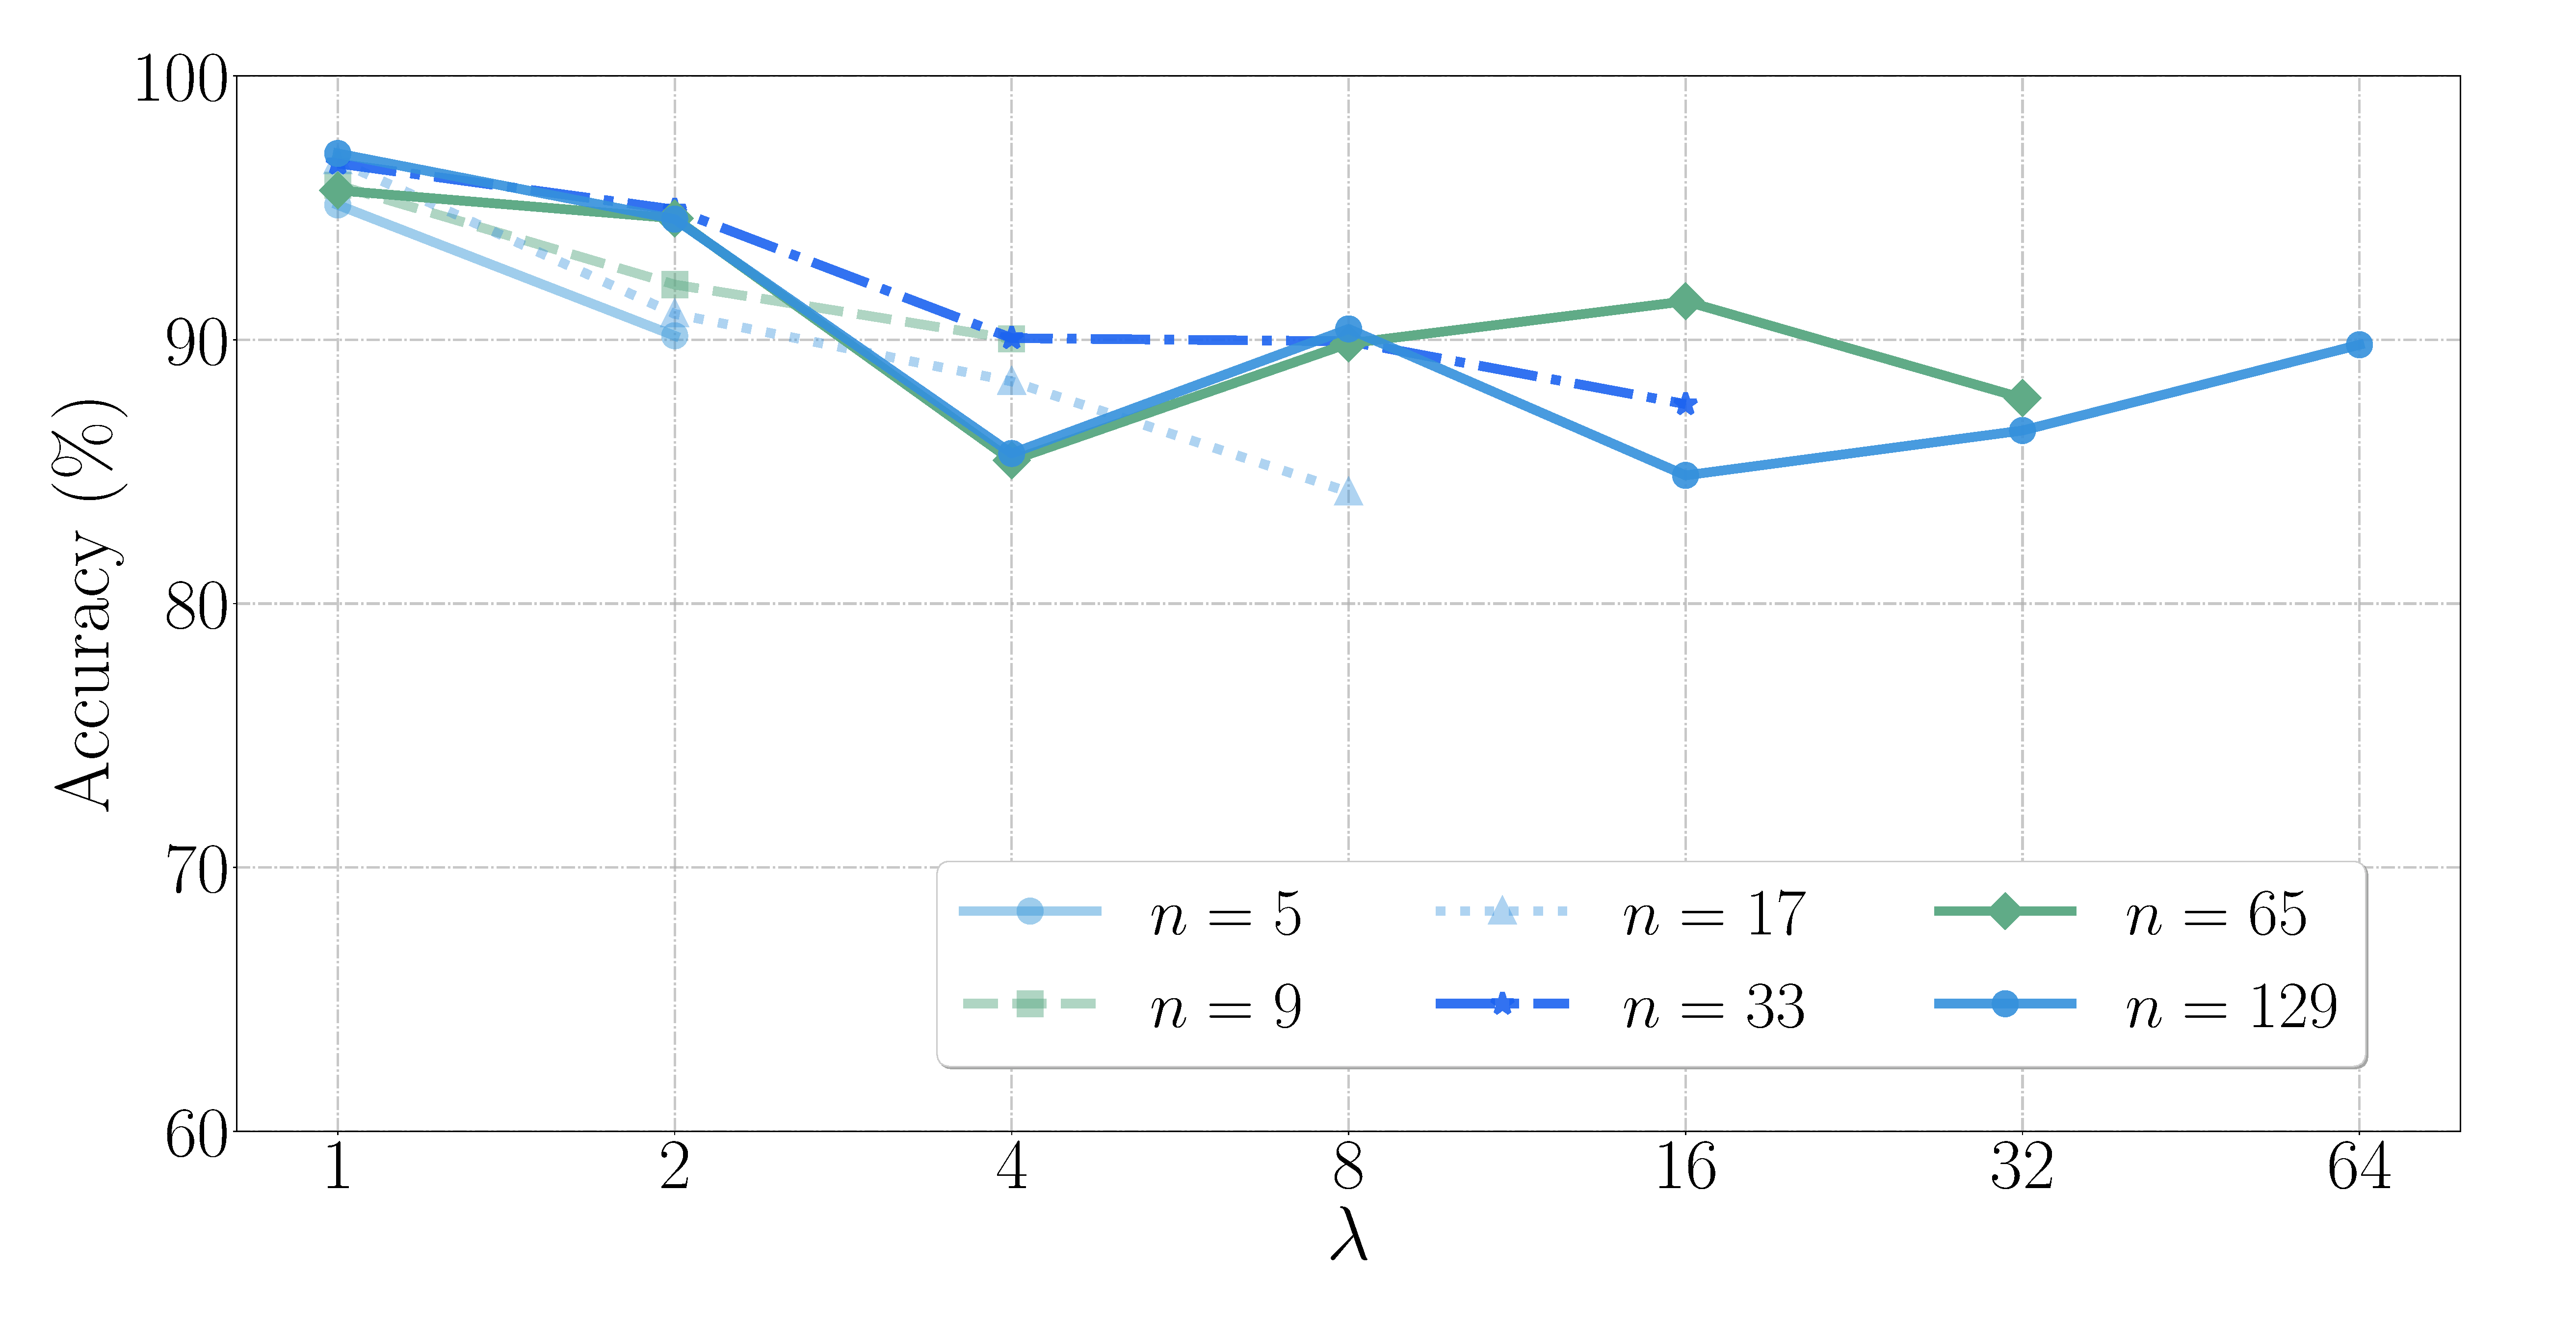
\includegraphics[width=1\linewidth]{latex/eval/DR.pdf}
    \caption{Accuracy of the feedback algorithm for different $\lambda$ and $n$ values under $f < \lceil \frac{n}{2} \rceil$.}
    \label{fig:dr}   
    \vspace{-19pt}
\end{figure}

\section{Analysis and Discussion}
\subsection{Enhancements}

Within the F-RCS framework, a general assumption is required. Consider the probability distributions produced by $n$ models over an output $y_h$ with unknown safety. After an arbitrary time interval $\Delta(t)$, if $y_h$ is determined to be unsafe, this means that the model state $\lvert \phi_h \rangle$ is unsafe. We require that the set of models $W$ that assign high probability to $y_h$ be trustworthy. Specifically, models in $W$ cannot deny the probability distributions reported before $\Delta(t)$. They also cannot modify the reported distributions. Models in $X$ cannot forge identities to impersonate models in $W$. These conditions can be enforced through cryptographic techniques such as blockchain \citep{Li2023FISCOBCOS, authors2018Fabric}. Such solutions are isomorphic to existing security supervision mechanisms for voting \citep{yang2021priscore}. Concrete designs tailored to F-RCS remain an open direction for future work.

For time cost optimization, we can construct an intermediate algorithm by trading off CS and RCS. One such example is RCS from local coins \citep{zhang2023waterbear}. After $R$ unsuccessful sampling rounds, the algorithm flips a coin to decide whether to return $\bot$ or to enter the trace phase. This design improves efficiency by sacrificing part of the safety. The detailed algorithm is provided in \autoref{app:Local Coin}.

\subsection{Additional Insights on Optimal Safety}

Based on experimental results, we observe a clear pattern. When $n$ is fixed, the SR of RCS often exhibits a maximum for different $\lambda$. For example, \autoref{fig:SR_m} shows a maximum at $\lambda = 8$. Very small values of $\lambda$ and very large values of $\lambda$ both fail to achieve optimal safety. For a fixed $n$, it is unclear both how to determine whether such a maximum exists and how to theoretically identify the value $\lambda_h$ corresponding to it.







\section{Related Work}

Existing research on generative AI security mainly focuses on the safety of model outputs. This line of work studies various attack methods \citep{li2024badedit, li2025one} and corresponding defenses \citep{zhang2025exploiting}. However, these attacks lack a unified definition of security. A representative example is the jailbreak attack \citep{mehrotra2024tree, zhang2025jbshield, yu2024don, wang-etal-2025-diffusionattacker}. This attack aims to induce models to generate unsafe content. Such content covers multiple categories \citep{guo2025deepseeknature}, including discrimination, illegal behavior, harmful behavior, and ethical issues. Output level unsafety is inherently subjective. This subjectivity prevents a deterministic definition under cryptographic theory. Current evaluation of output safety largely relies on LLM-as-a-judge \citep{li-etal-2025-generation}. This approach depends on specialized evaluator models trained for safety analysis, such as Qwen3Guard \citep{zhao2025qwen3guard}. These models perform semantic analysis on generated content. However, evaluator models are not interpretable. Their correctness in safety assessment cannot be formally proven. Defenses against these attacks also lack formal guarantees. As a result, research on generative model security lacks a mature theoretical foundation. This absence of theory leads to inconsistent standards across existing attack and defense studies. 
% In contrast, our work provides a theoretical guarantee, ensuring that the delivered response admits an upper bound on risk.



\section{Conclusion}
In this paper, we formalize a provable security theory for model groups. We introduce RCS, a trace-based method that eliminates abstention and guarantees effective delivery. RCS can tolerate extreme adversarial behavior. We also design a feedback algorithm to improve RCS safety. We prove that RCS has tight upper bounds on response risk. Experiments show that RCS outperforms CS in robustness and utility, achieving a $5\times$ increase in safety rate, while maintaining comparable latency.

\section{Limitations and Ethical Considerations}
In this paper, we employ a safety threshold $f < \lceil \frac{n}{2} \rceil$ in traditional consensus sampling. Although this condition is feasible and justified in real-world deployments, exploring looser thresholds, such as $f < \lceil \frac{2n}{3} \rceil$, remains to be explored in future work. In addition, our discussion on unsafe models covers various adversarial behaviors of Byzantine models. However, more extreme threats warrant further study in future work. The Byzantine behavior discussed in this paper may be harmful. The methods described in this paper may be used for research purposes only.

% Bibliography entries for the entire Anthology, followed by custom entries
%\bibliography{anthology,custom}
% Custom bibliography entries only
\bibliography{acl_latex}
\onecolumn
\newpage

\appendix

\section{RCS from Local Coins}
\label{app:Local Coin}

\begin{algorithm}[h]
\SetAlgoLined
\KwIn{
Number of models $|\mathcal{MG}|=n$; number of safe models $s$; 
round $R$; distributions $p_1, \ldots, p_n \in \mathrm{Distr}(\mathcal{Y})^{n}$
}
\KwOut{Response $y \in \mathcal{Y}$}

$Buffer \gets \varnothing$\\
\For{$r \leftarrow 1$ \KwTo $R$}{
    Sample $y \sim \frac{1}{n}\sum_{i=1}^{n} p_i$ \\
    $\sigma(y) =\frac{\frac{1}{s}\sum_{i=1}^{s} p_{(i)}(y)}
             {\frac{1}{n}\sum_{i=1}^{n} p_i(y)}$
        
    \If{accept $y$ with $\sigma(y)$}{
        \Return $y$
    }
    $Buffer \gets Buffer \cup \{\langle y, \sigma(y) \rangle \}$\\
}
$c \gets Random()$ \textcolor{mGreen}{\#Obtain local coin 0 or 1.} \\
\If{$c==0$}{
\Return $\bot$
}\Else{

Sort $Buffer=\{\langle y_i, \sigma(y_i) \rangle \}_{i=1}^{R}$ 
 such that $\sigma(y_{(1)}) \ge \dots \ge \sigma(y_{(R)})$\\
Let $\mathcal{F} = \{y_{(1)}, \dots, y_{u}\}, \; u= min(s,R)$ \\
\For{$i \leftarrow 1$ \KwTo $u$}{
    $\alpha(y_{(i)}) = \sum_{j=s+1}^{n} p_{(j)}(y_{(i)})$
}
\Return $y \gets \arg\max_{y \in \mathcal{F}} \alpha(y)$

}


\caption{Reliable Consensus Sampling from Local Coins}
\label{alg:coin}
\end{algorithm}



\section{Proof}
\label{app:ac}

\begin{align*}
&\sigma(y_t) - \sigma(y_v) \\
&=
\frac{\frac{1}{s} \sum_{i \le s} p_{(i)}(y_t)}
     {\frac{1}{n} \sum_{i=1}^{n} p_i(y_t)}
-
\frac{\frac{1}{s} \sum_{i \le s} p_{(i)}(y_v)}
     {\frac{1}{n} \sum_{i=1}^{n} p_i(y_v)}
\\[2mm]
&=
\frac{
\left( \frac{1}{s} \sum_{i \le s} p_{(i)}(y_t) \right)
\left( \frac{1}{n} \sum_{i=1}^{n} p_i(y_v) \right)
-
\left( \frac{1}{s} \sum_{i \le s} p_{(i)}(y_v) \right)
\left( \frac{1}{n} \sum_{i=1}^{n} p_i(y_t) \right)
}{
\left( \frac{1}{n} \sum_{i=1}^{n} p_i(y_t) \right)
\left( \frac{1}{n} \sum_{i=1}^{n} p_i(y_v) \right)
}
\\[2mm]
&=
\frac{n}{s} \cdot
\frac{
\left( \sum_{i \le s} p_{(i)}(y_t) \right)
\left( \sum_{i=1}^{n} p_i(y_v) \right)
-
\left( \sum_{i \le s} p_{(i)}(y_v) \right)
\left( \sum_{i=1}^{n} p_i(y_t) \right)
}{
\left( \sum_{i=1}^{n} p_i(y_t) \right)
\left( \sum_{i=1}^{n} p_i(y_v) \right)
}
\\[2mm]
% &=
% \frac{n}{s} \cdot
% \frac{
% \left( \sum_{i \le s} p_{(i)}(y_t) \right)
% \left(
% \sum_{i \le s} p_{(i)}(y_v)
% +
% \sum_{i > s} p_{(i)}(y_v)
% \right)
% -
% \left( \sum_{i \le s} p_{(i)}(y_v) \right)
% \left(
% \sum_{i \le s} p_{(i)}(y_t)
% +
% \sum_{i > s} p_{(i)}(y_t)
% \right)
% }{
% \left( \sum_{i=1}^{n} p_i(y_t) \right)
% \left( \sum_{i=1}^{n} p_i(y_v) \right)
% }
% \\[2mm]
&=
\frac{n}{s} \cdot
\frac{
\left( \sum_{i \le s} p_{(i)}(y_t) \right)
\left( \sum_{i > s} p_{(i)}(y_v) \right)
-
\left( \sum_{i \le s} p_{(i)}(y_v) \right)
\left( \sum_{i > s} p_{(i)}(y_t) \right)
}{
\left( \sum_{i=1}^{n} p_i(y_t) \right)
\left( \sum_{i=1}^{n} p_i(y_v) \right)
}
\end{align*}


\section{Additional Discussion}
\subsection{RCS and Multi-Agent Debate}

Multi-agent debate (MAD) \citep{du2024improving, chan2024chateval, liu2025breaking} is a reasoning enhancement technique built on LLM inference. MAD enables multiple agents to interact over several rounds. The goal is to encourage consensus on the same answer to a given query. A final decision is then produced through answer aggregation methods such as majority voting \citep{du2024improving}. In terms of output safety, MAD and RCS share a similar motivation. Both approaches introduce multiple models to improve the safety of the final output. Some MAD methods also adopt confidence scores to evaluate candidate answers proposed by other models \citep{chen-etal-2024-reconcile}. This mechanism is conceptually related to RCS. Compared to MAD, RCS follows a more fundamental strategy. RCS directly operates on underlying probability distributions. In contrast, MAD requires models to possess an explicit understanding of safety. This requirement limits robustness against unforeseen attacks. Moreover, RCS does not require interaction among models. This design avoids the conformity \citep{weng2025do} inherent in LLMs. Operating on underlying probability distributions also mitigates the impact of hallucination \citep{ji-etal-2023-towards} during reasoning. However, this design limits practical applicability. In many scenarios, models are accessed as black-box services, and probability distributions are not available. We argue that an intersection between MAD and RCS can improve the practical applicability of RCS. We continue to avoid direct interaction among models. Instead, each model outputs a score for each candidate output $y$ at every round. This score represents the level of support for $y$. All other components remain consistent with RCS. We refer to this variant as Practical Reliable Consensus Sampling (PRCS). More broadly, PRCS can be applied beyond safety. It can also enhance model reasoning performance in domains such as mathematics, medicine, and programming \citep{luo2025large}.

\section{Additional Experimental Results}
\label{app:results}
\begin{figure*}[h]
    \centering
    \begin{subfigure}{0.31\textwidth}
        \centering
        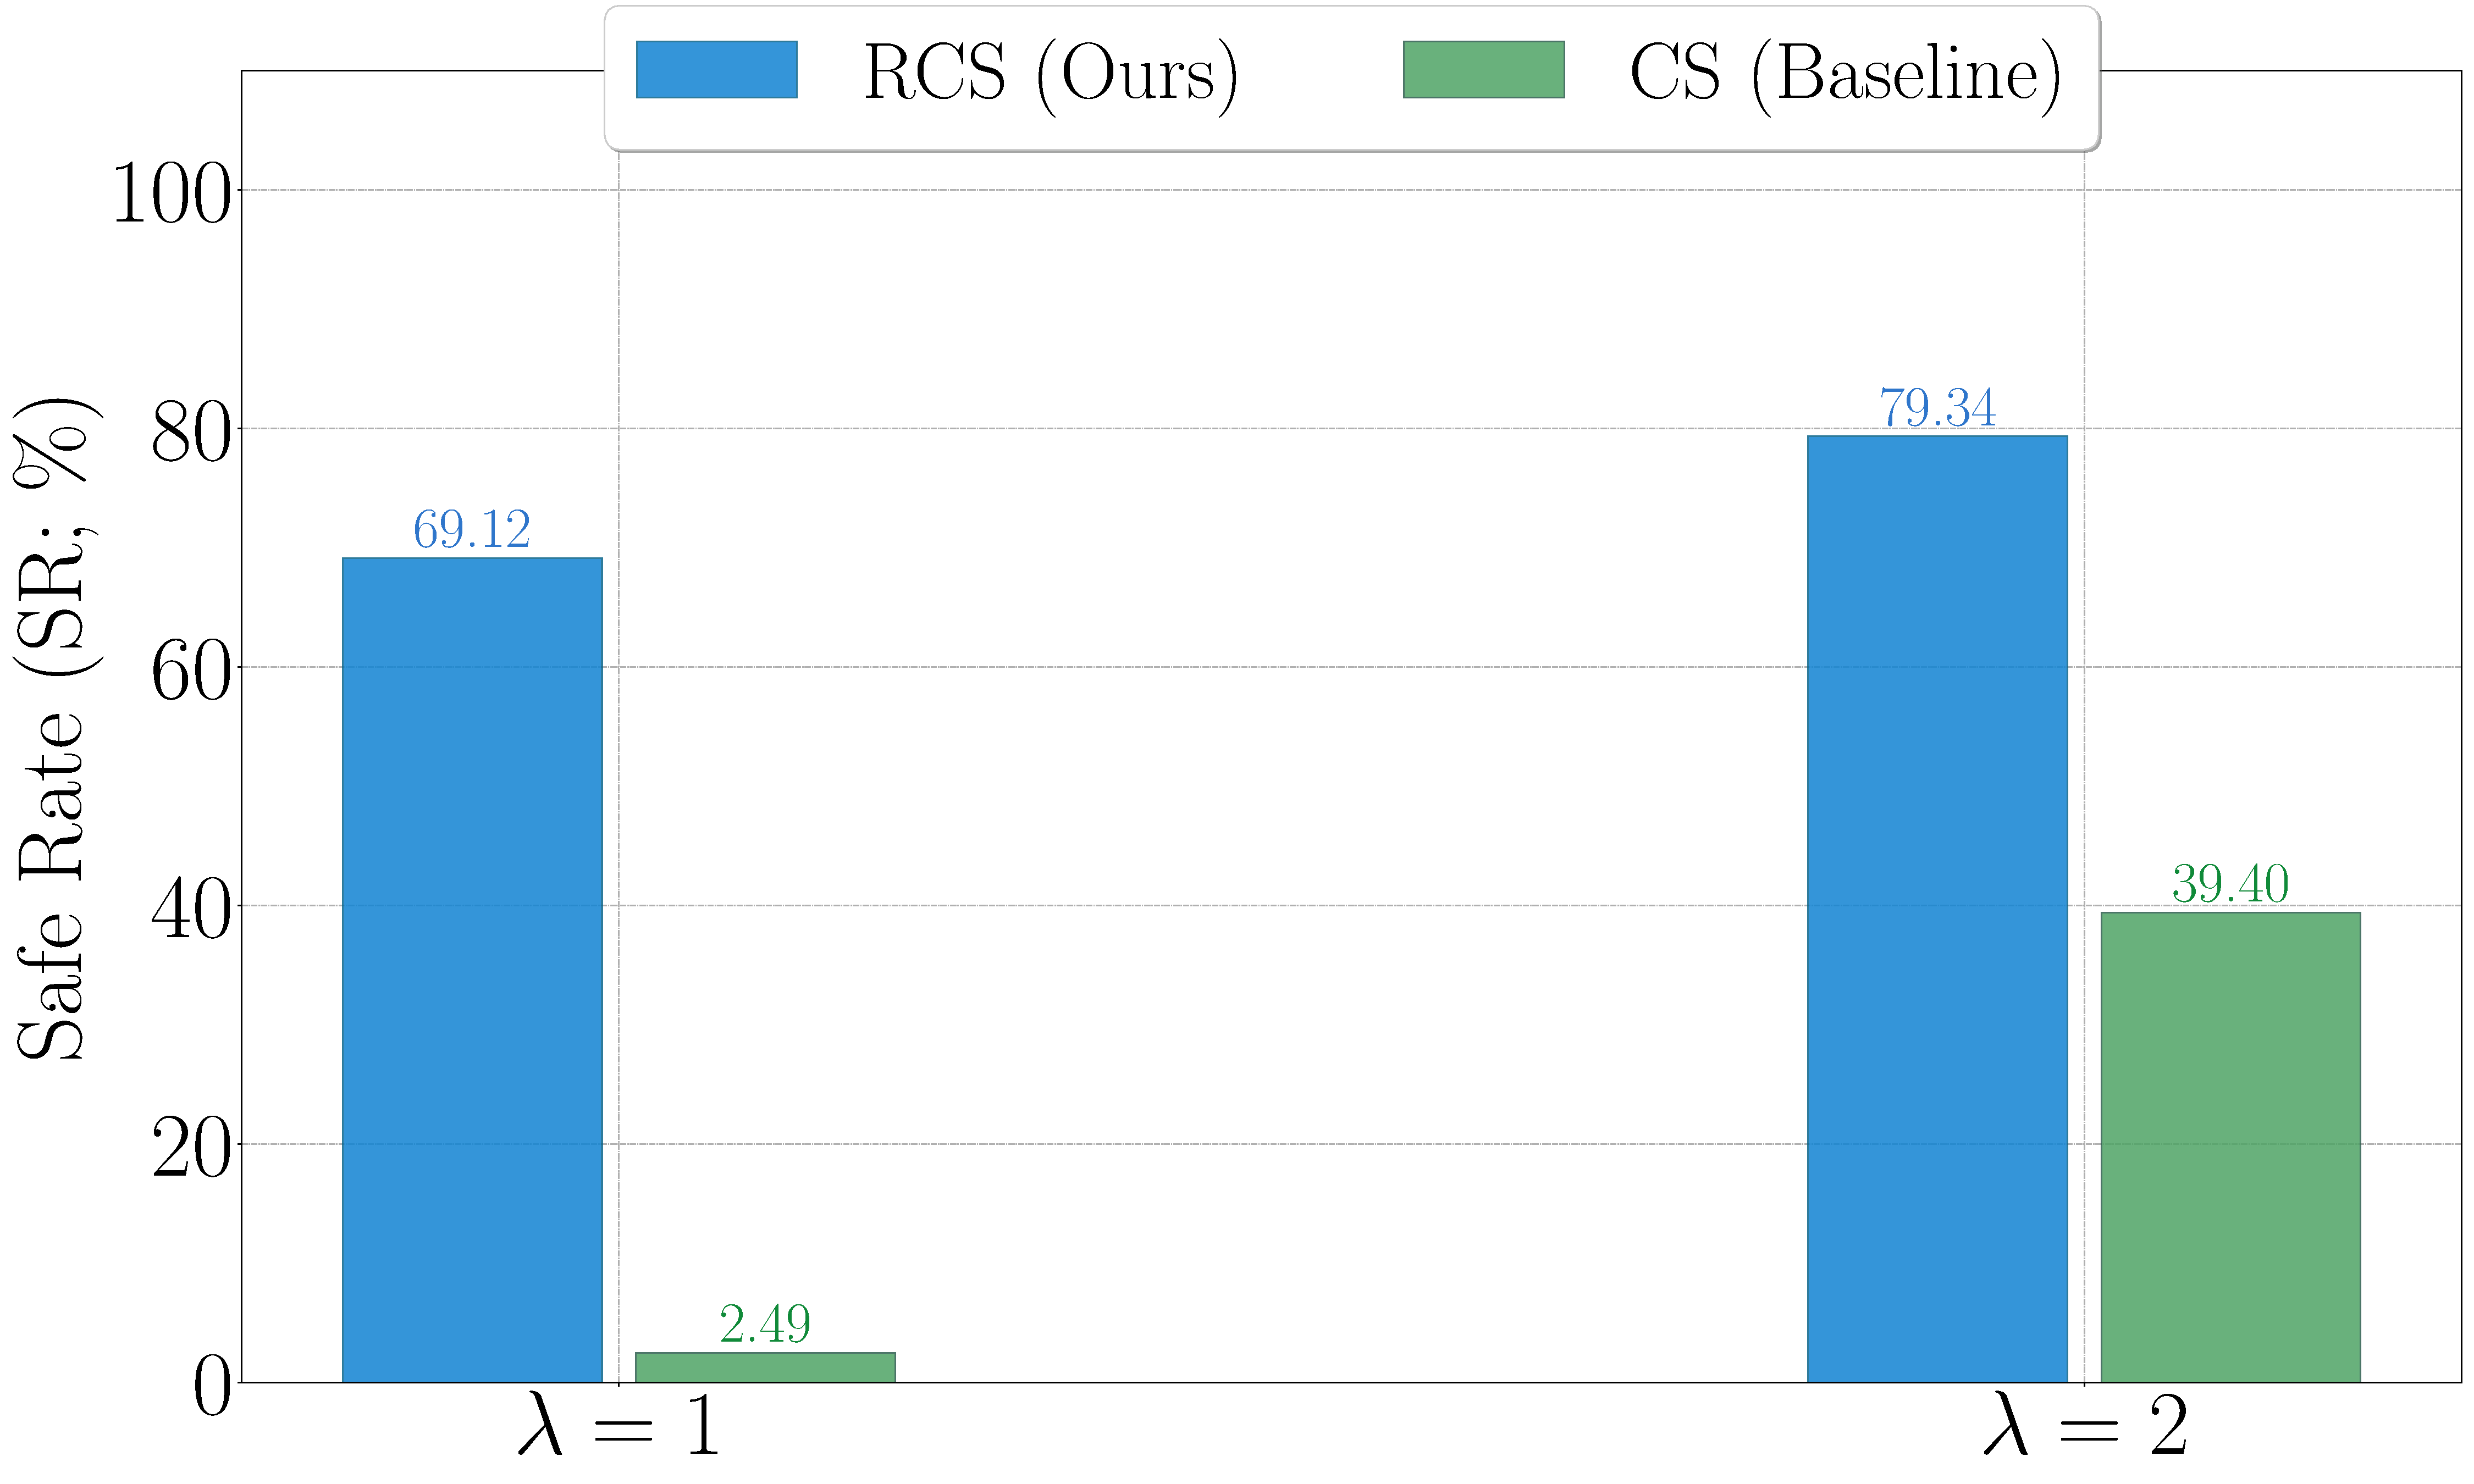
\includegraphics[width=\linewidth]{latex/eval_res/SR-5.pdf}
        \caption{$n=5$.}
    \end{subfigure}
    \begin{subfigure}{0.31\textwidth}
        \centering
        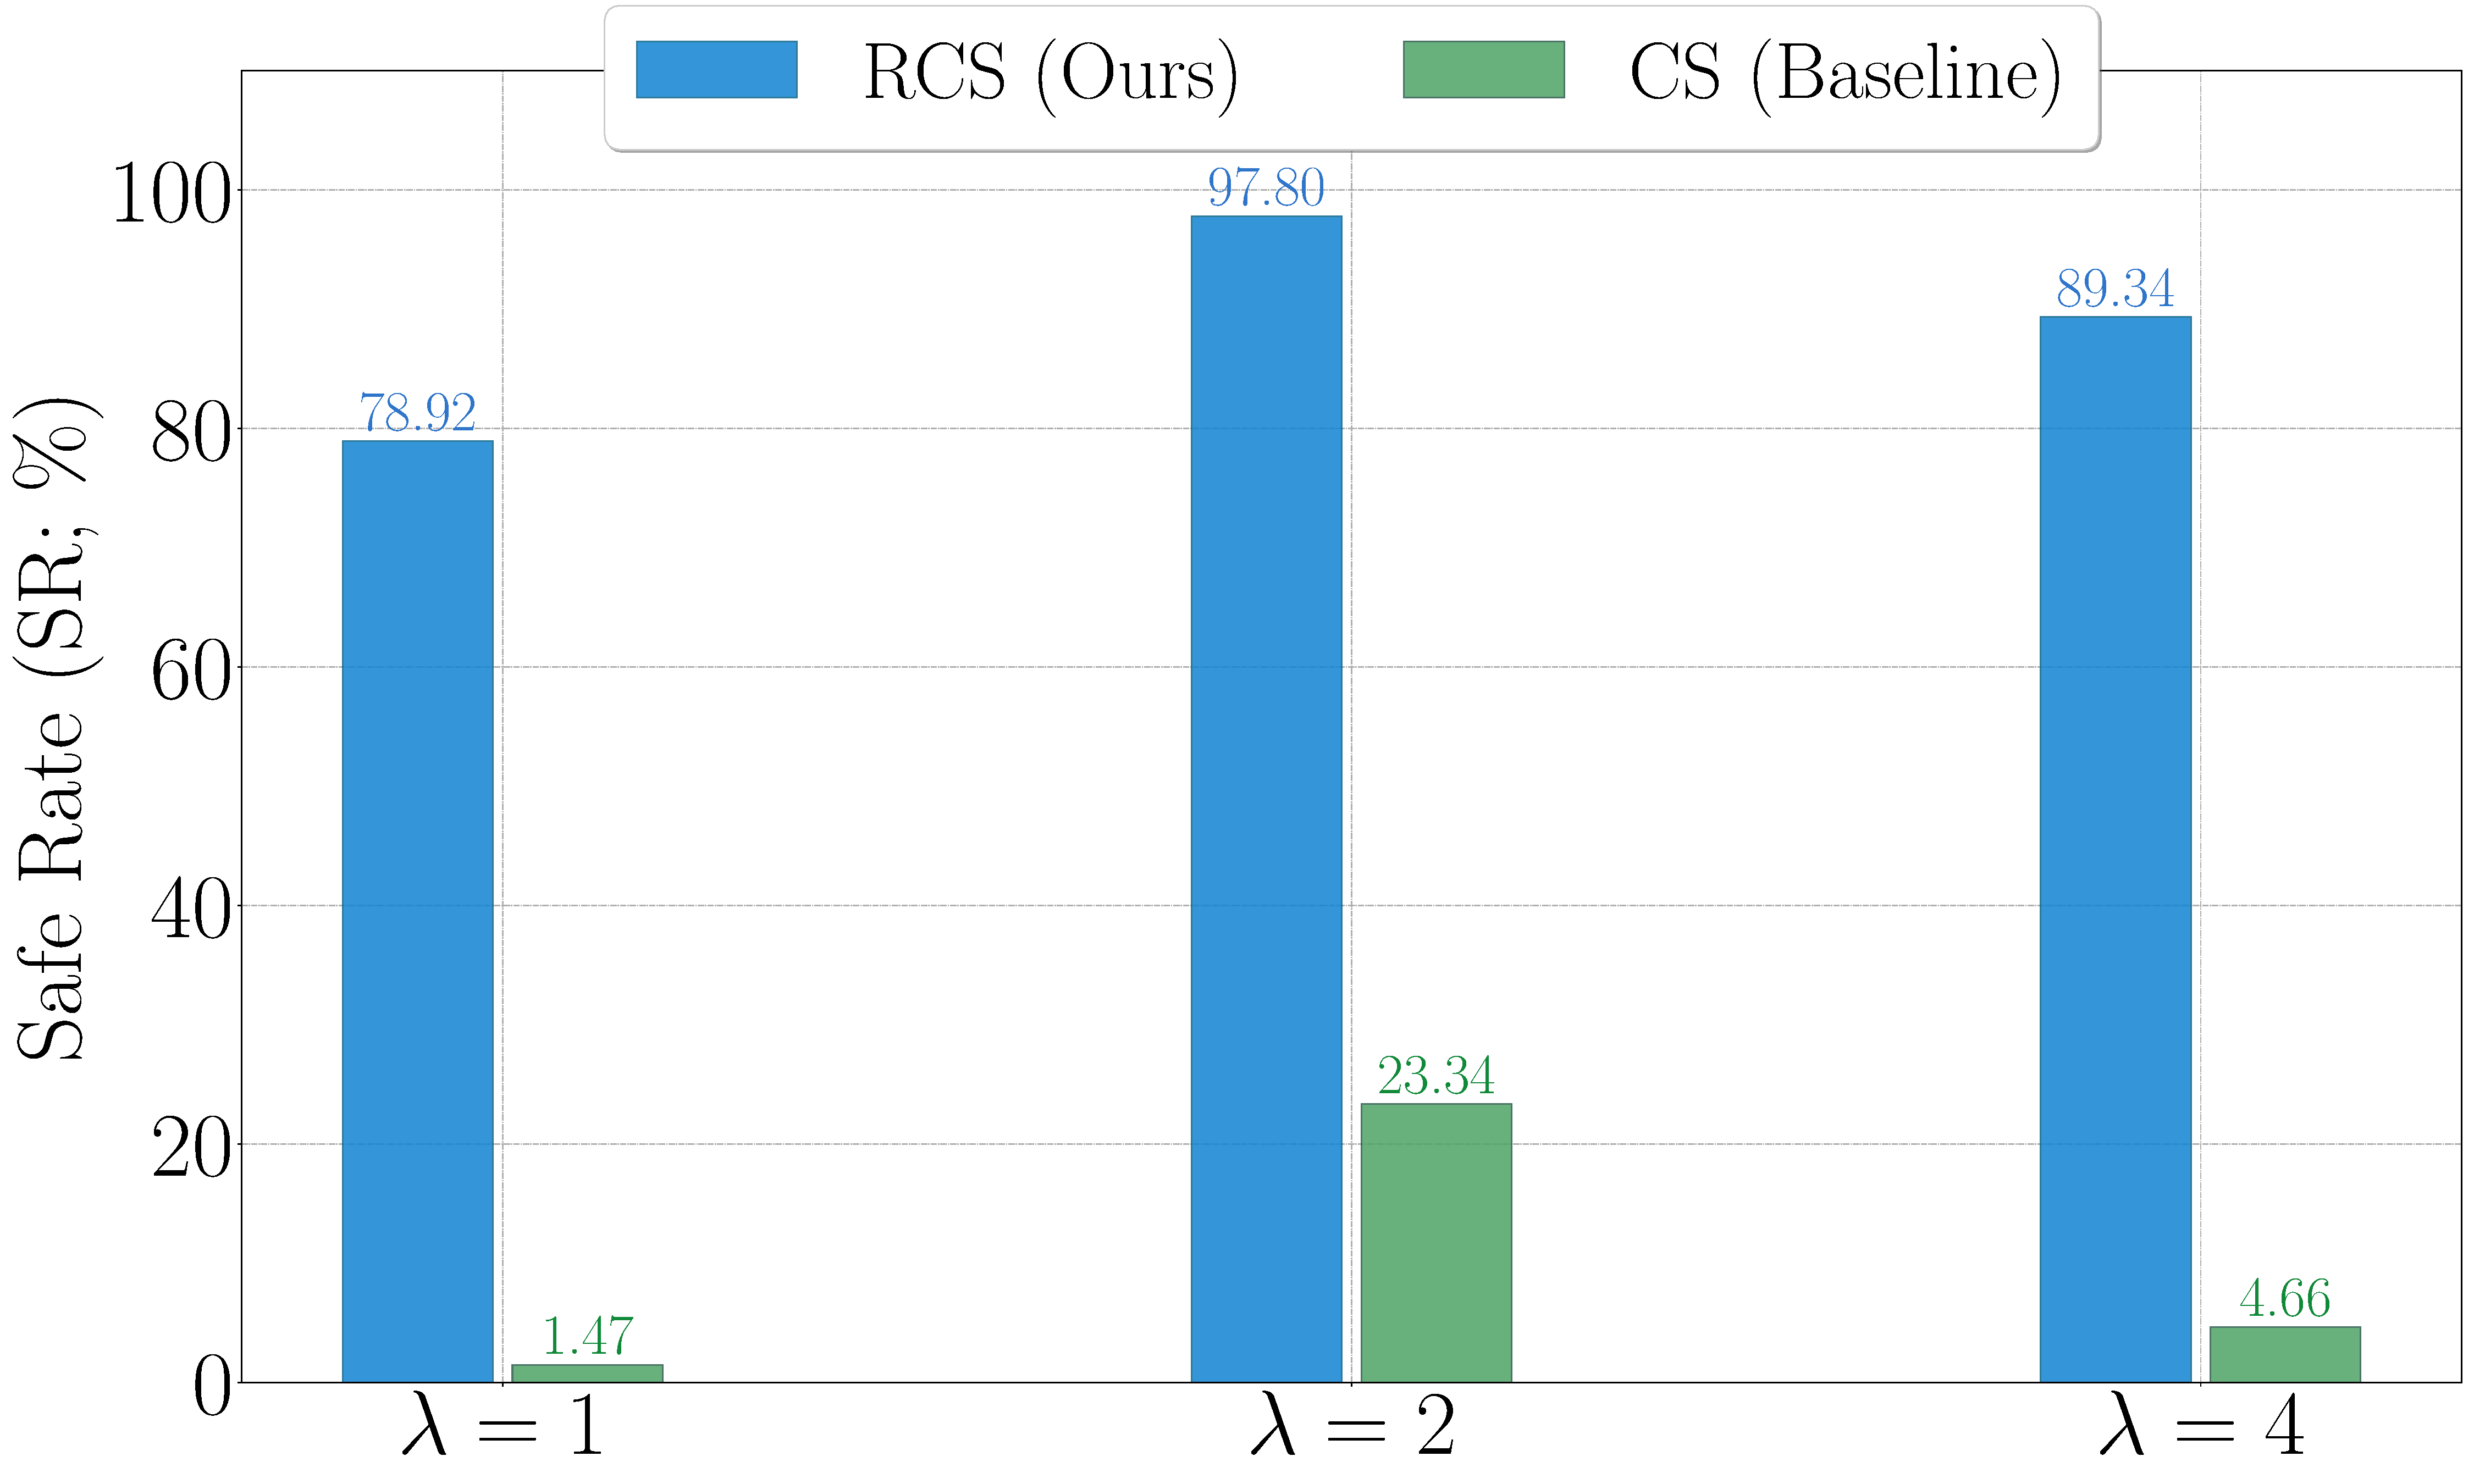
\includegraphics[width=\linewidth]{latex/eval_res/SR-9.pdf}
        \caption{$n=9$.}
    \end{subfigure}
    \begin{subfigure}{0.31\textwidth}
        \centering
        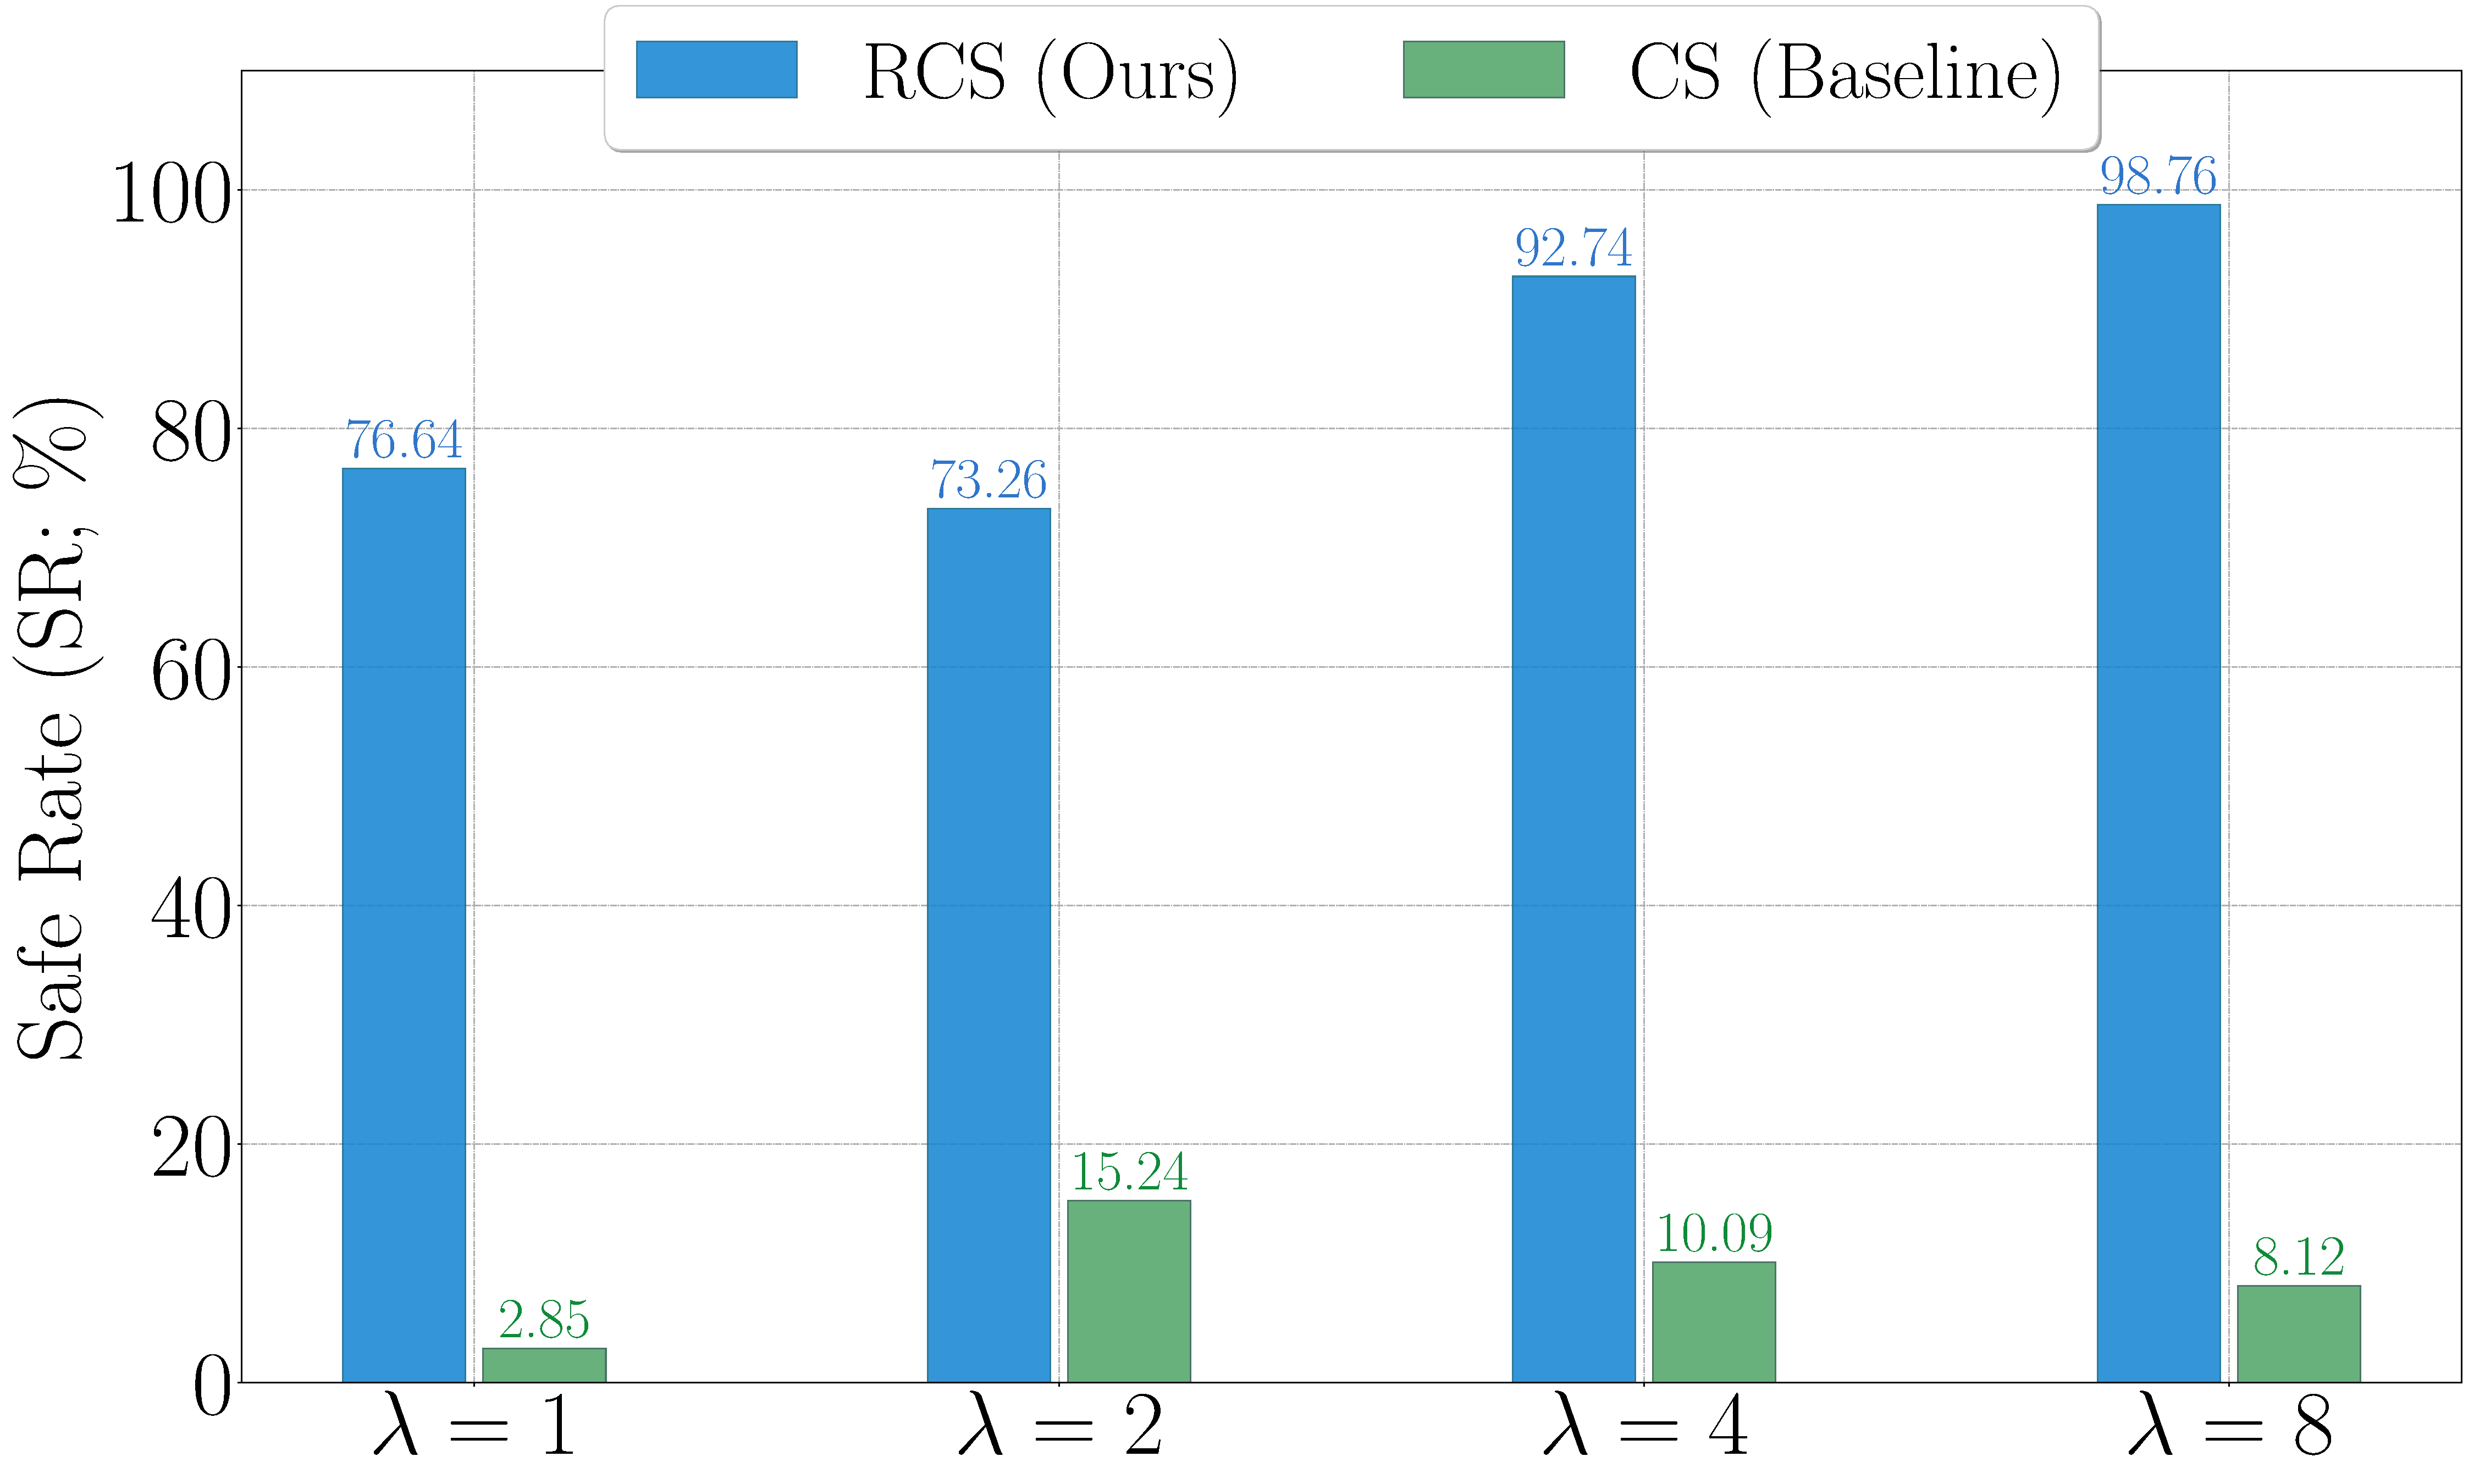
\includegraphics[width=\linewidth]{latex/eval_res/SR-17.pdf}
        \caption{$n=17$.}
    \end{subfigure}
    \caption{Evaluation results for the safe rate when $f < \lceil \frac{n}{2} \rceil$.}
    \label{fig:sr_app}
    \vspace{-15pt}
\end{figure*}


\begin{figure*}[h]
    \centering
    \begin{subfigure}{0.31\textwidth}
        \centering
        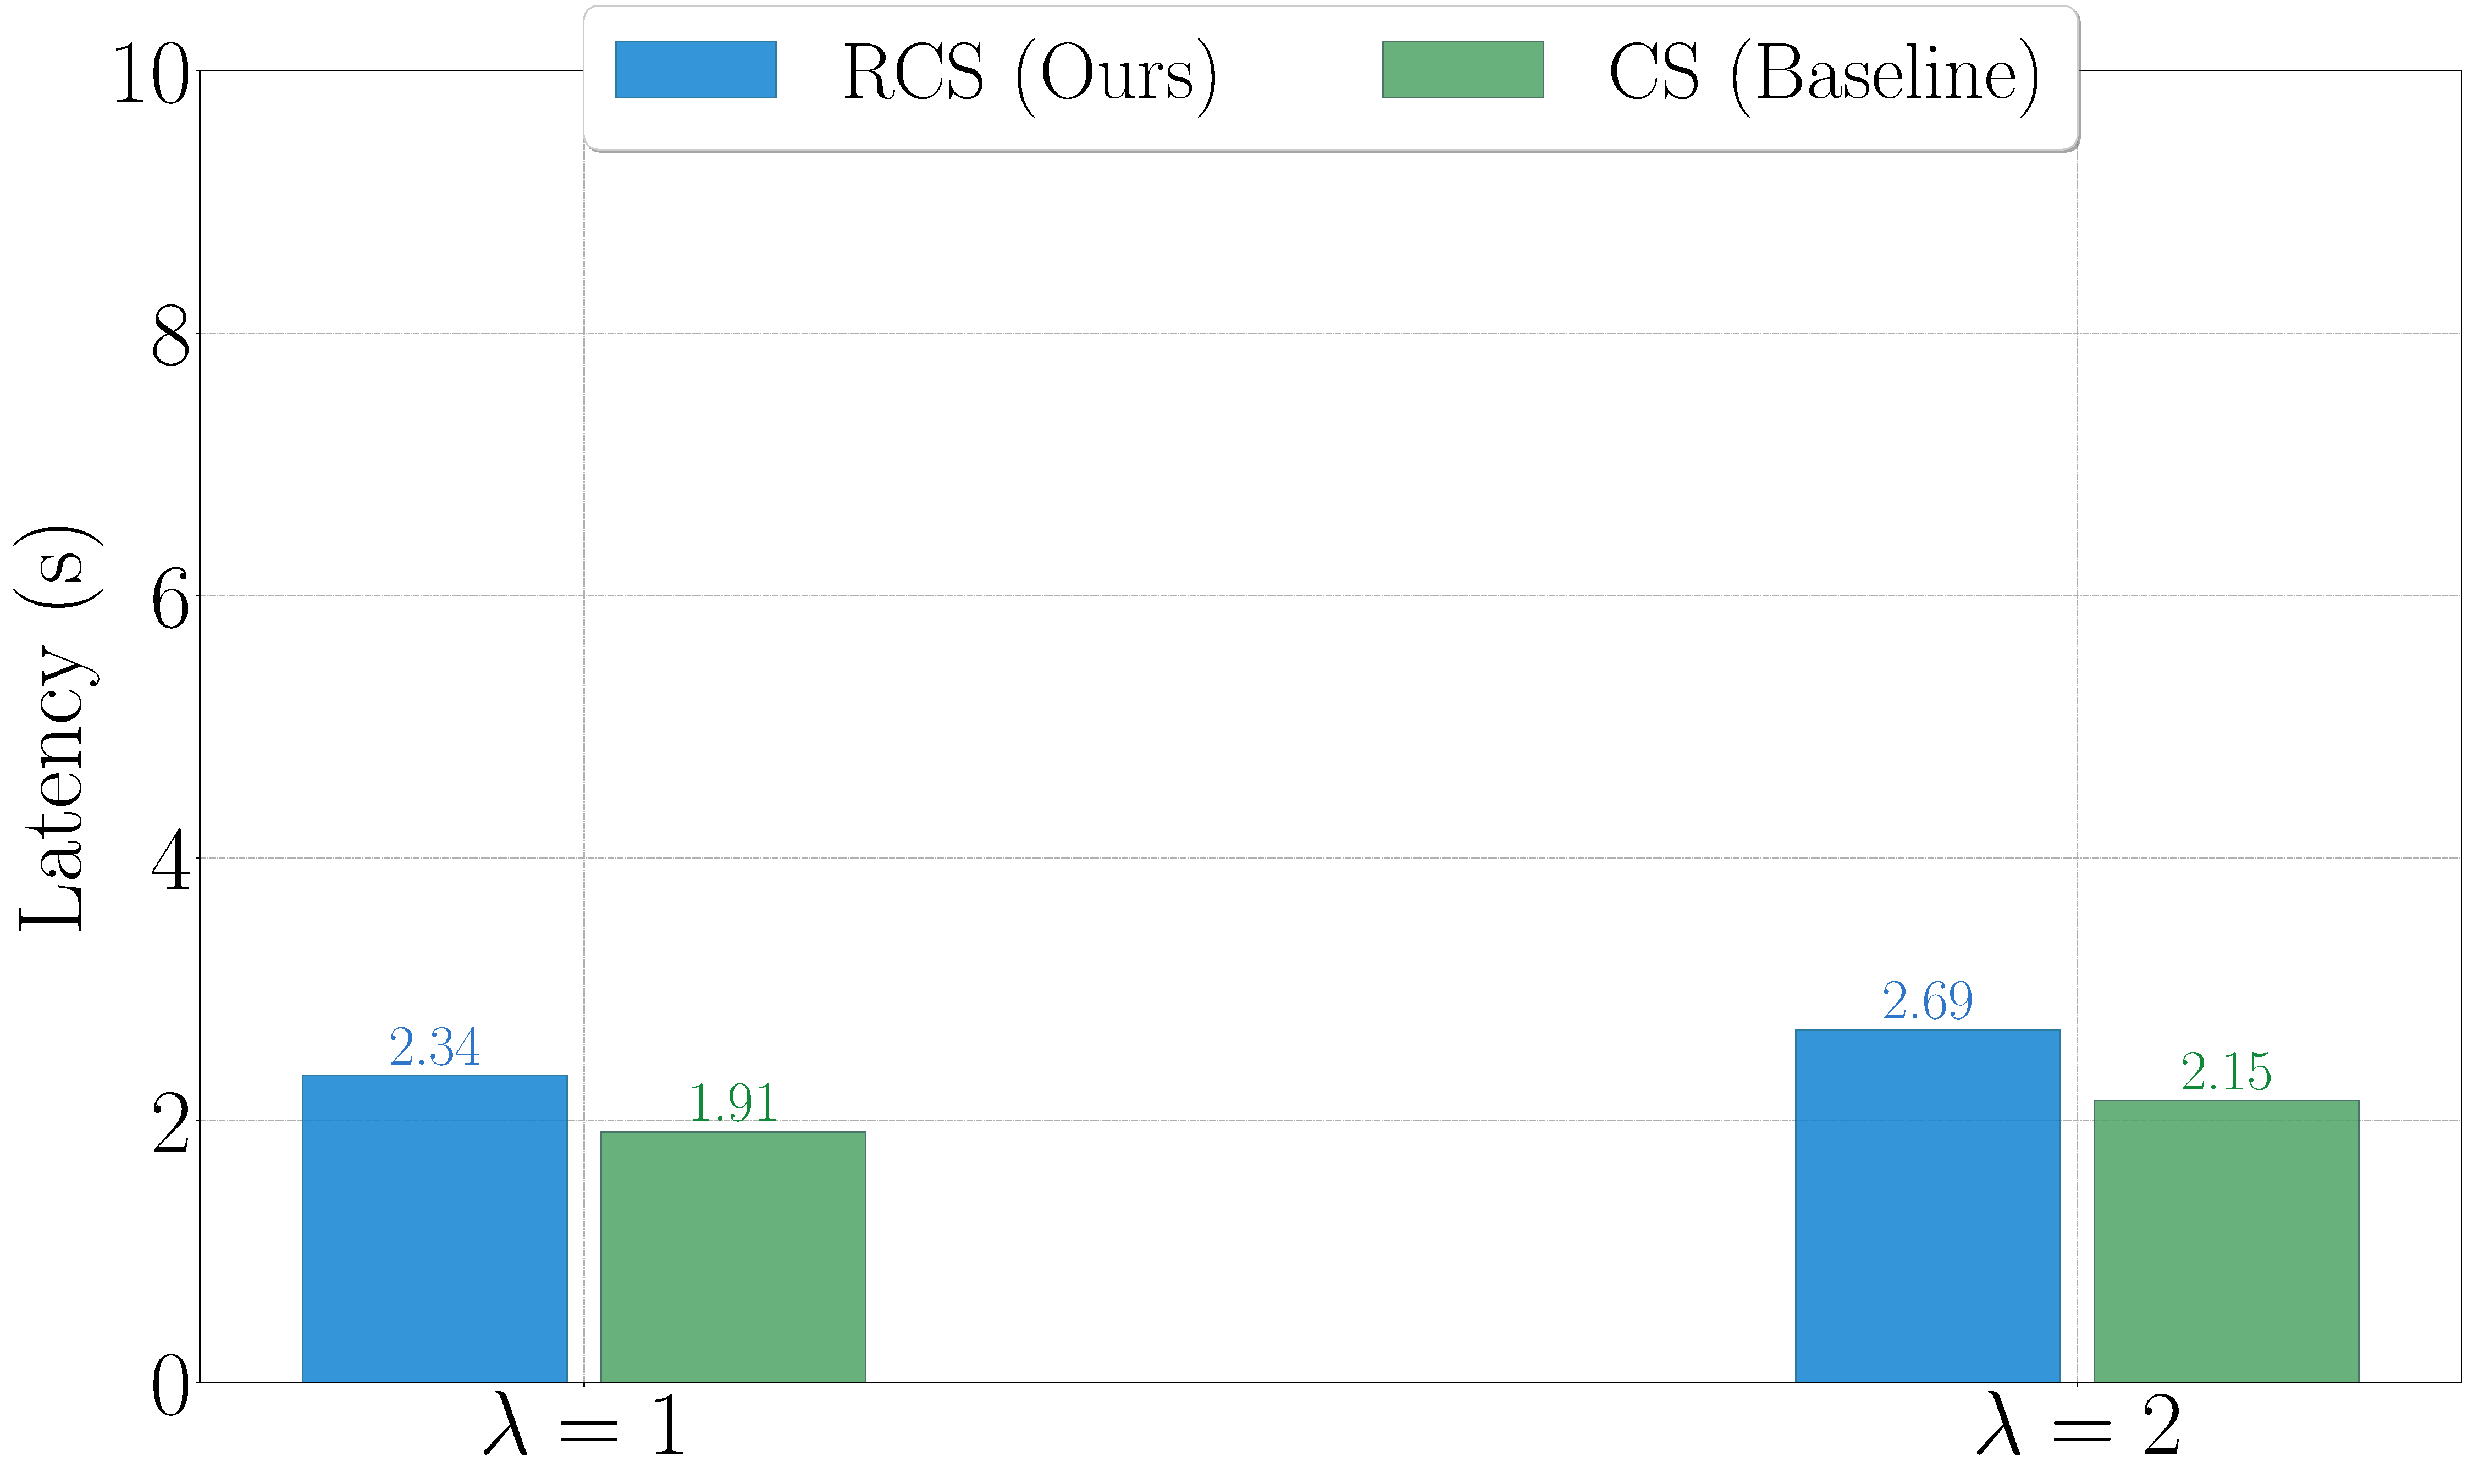
\includegraphics[width=\linewidth]{latex/eval_res/TC-5.pdf}
        \caption{$n=5$.}
    \end{subfigure}
    \begin{subfigure}{0.31\textwidth}
        \centering
        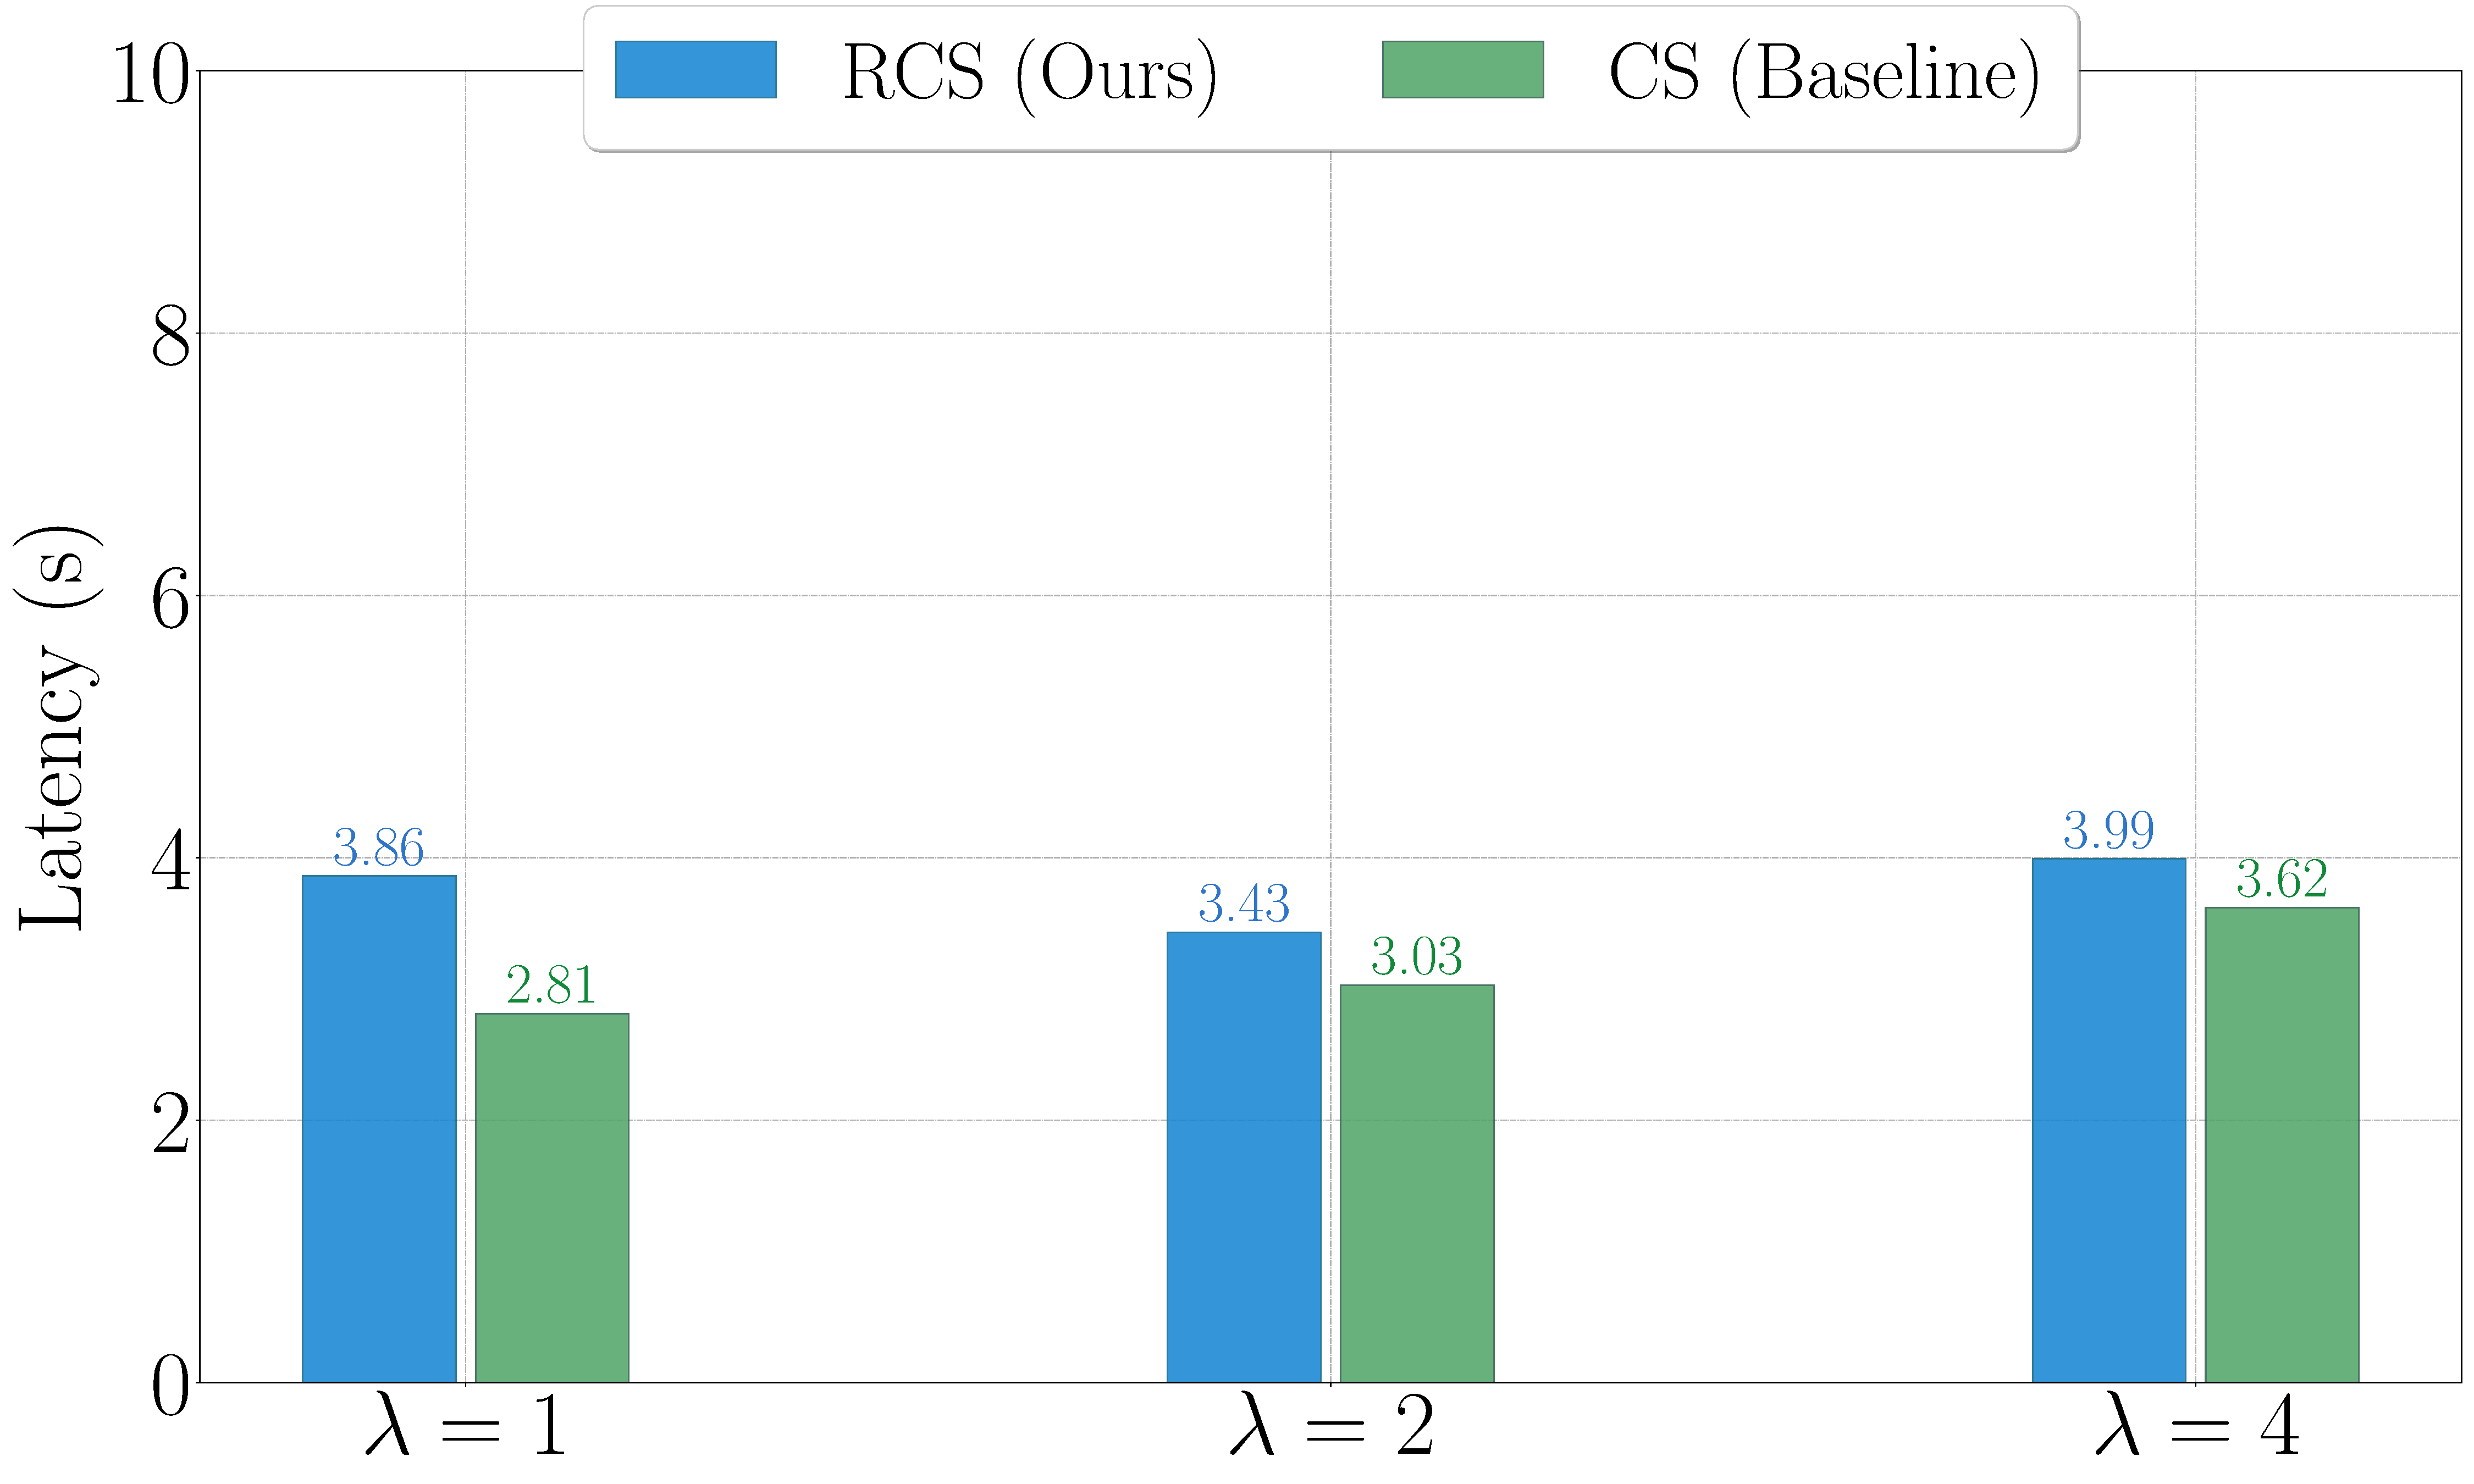
\includegraphics[width=\linewidth]{latex/eval_res/TC-9.pdf}
        \caption{$n=9$.}
    \end{subfigure}
    \begin{subfigure}{0.31\textwidth}
        \centering
        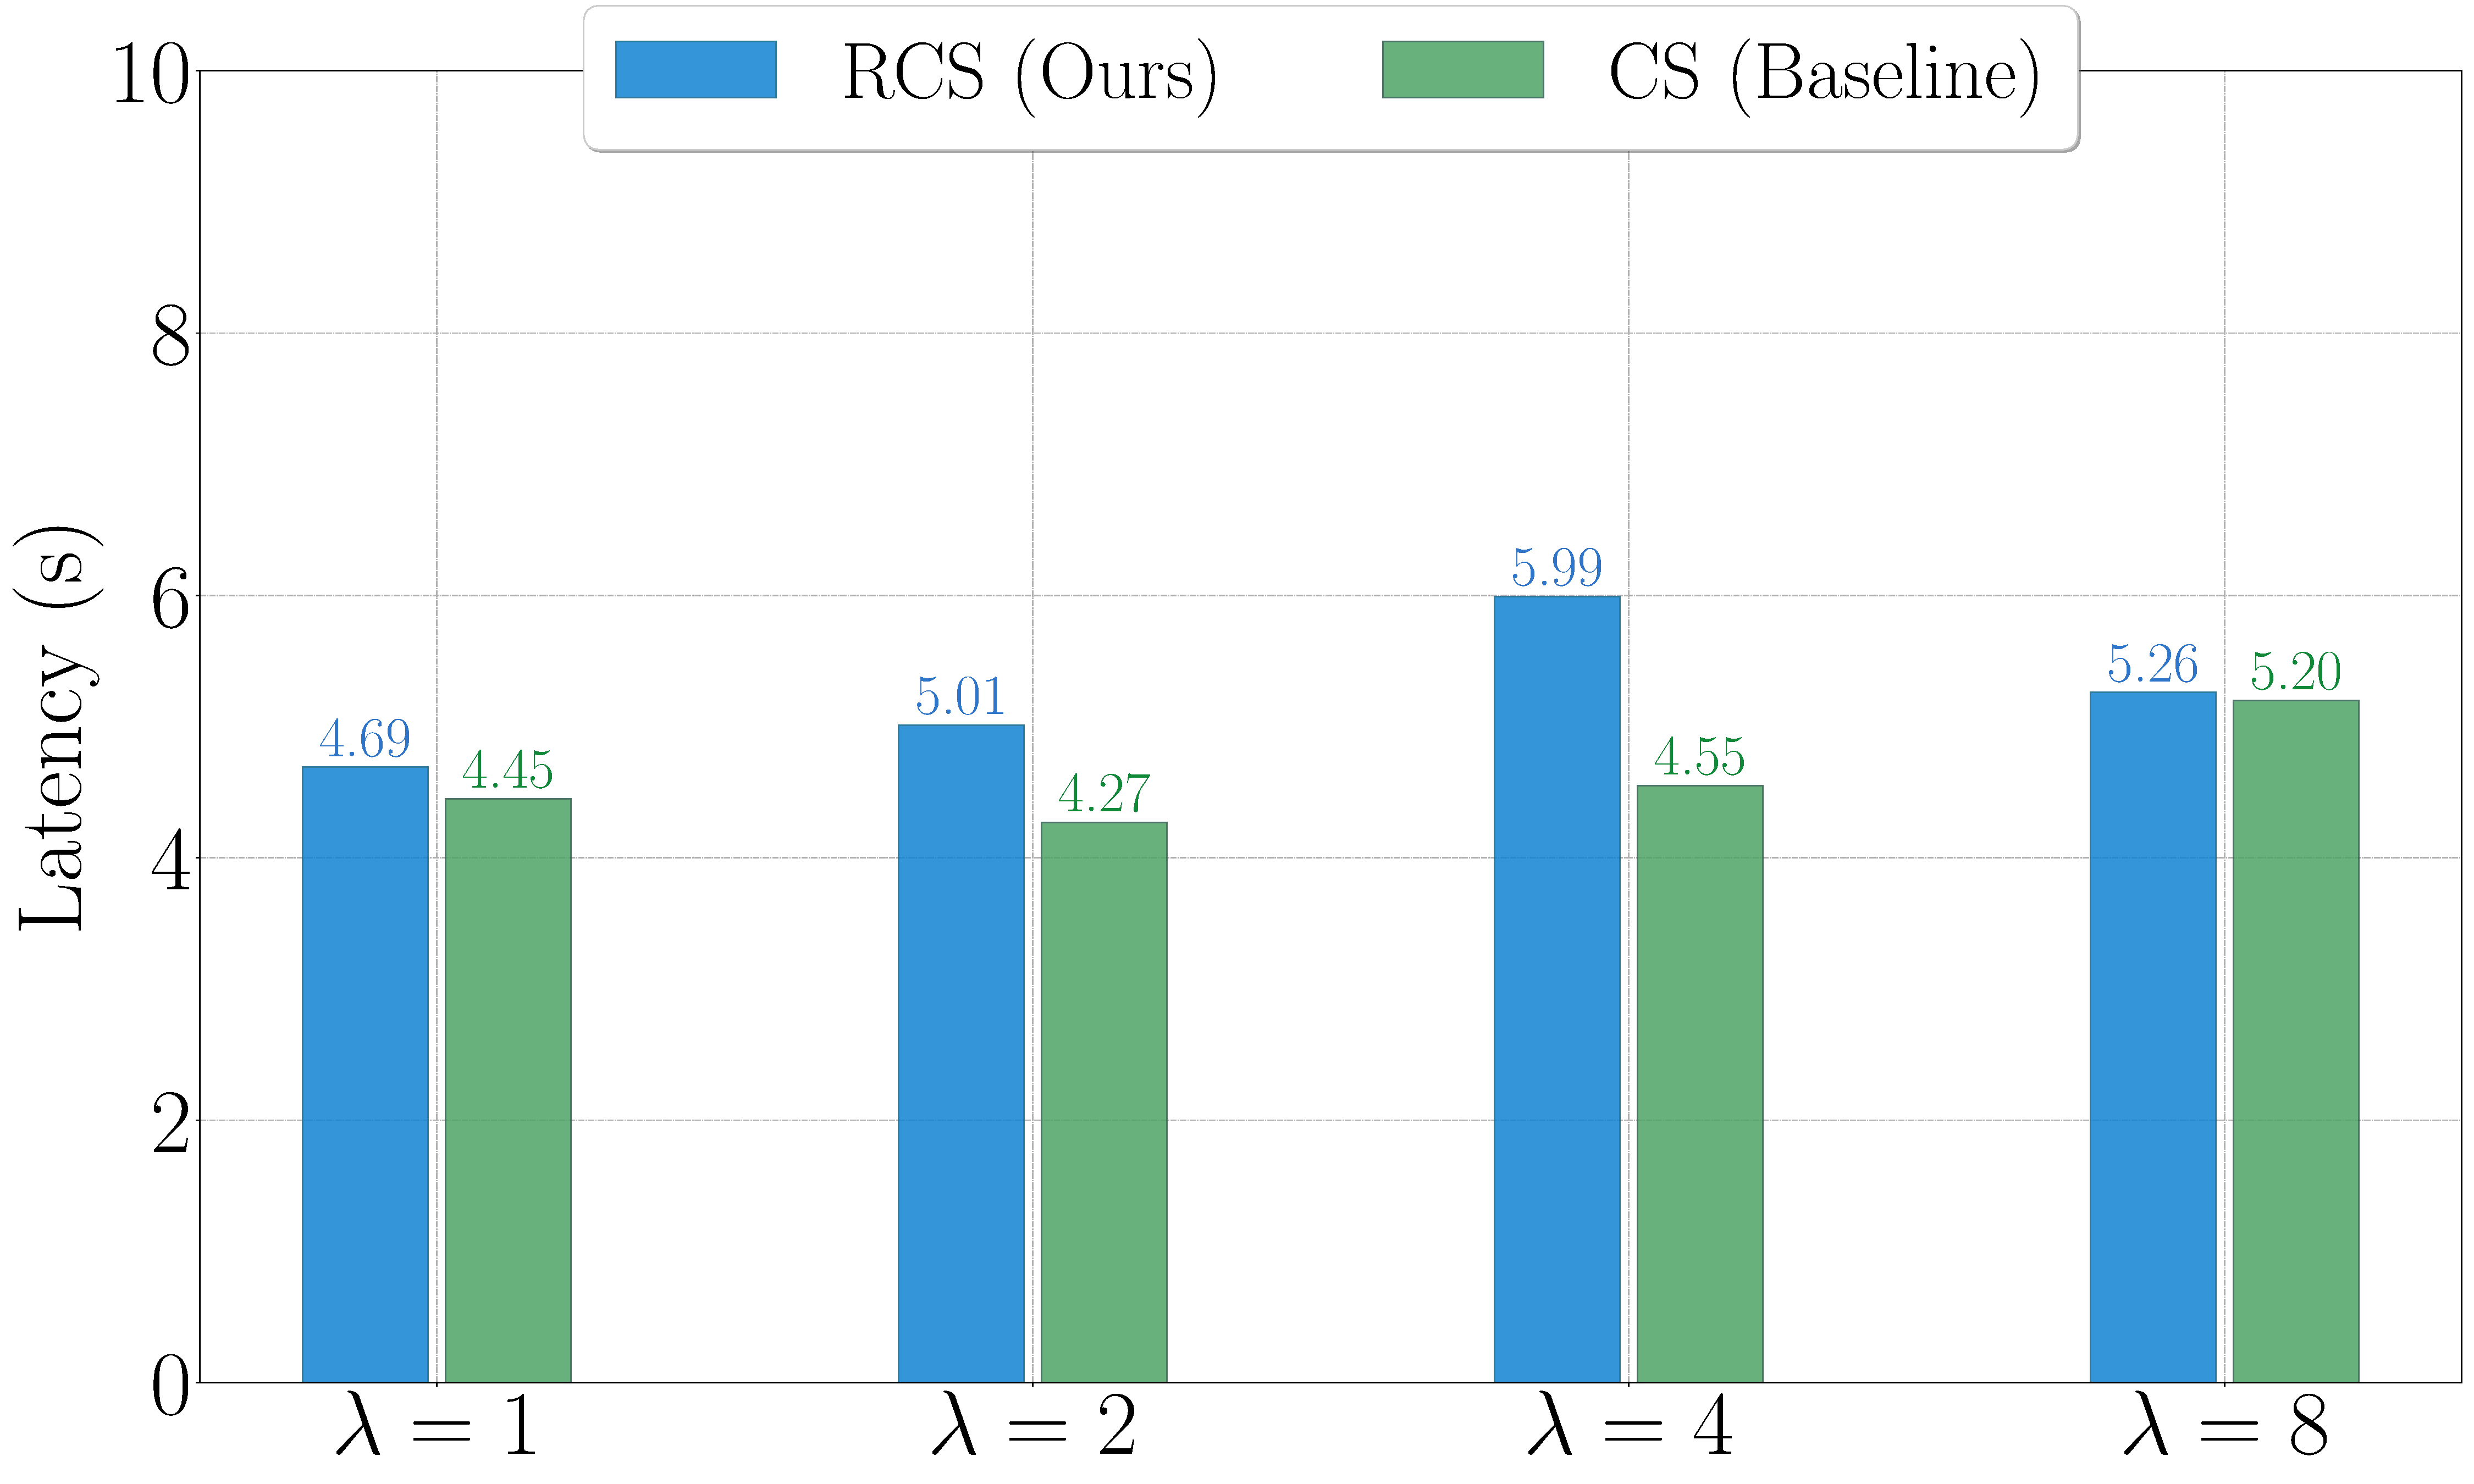
\includegraphics[width=\linewidth]{latex/eval_res/TC-17.pdf}
        \caption{$n=17$.}
    \end{subfigure}
    \caption{Evaluation results for the latency when $f < \lceil \frac{n}{2} \rceil$.}
    \label{fig:TC_g_app}
    % \vspace{-15pt}
\end{figure*}



\begin{figure*}[h]
    \centering
    \begin{subfigure}{0.31\textwidth}
        \centering
        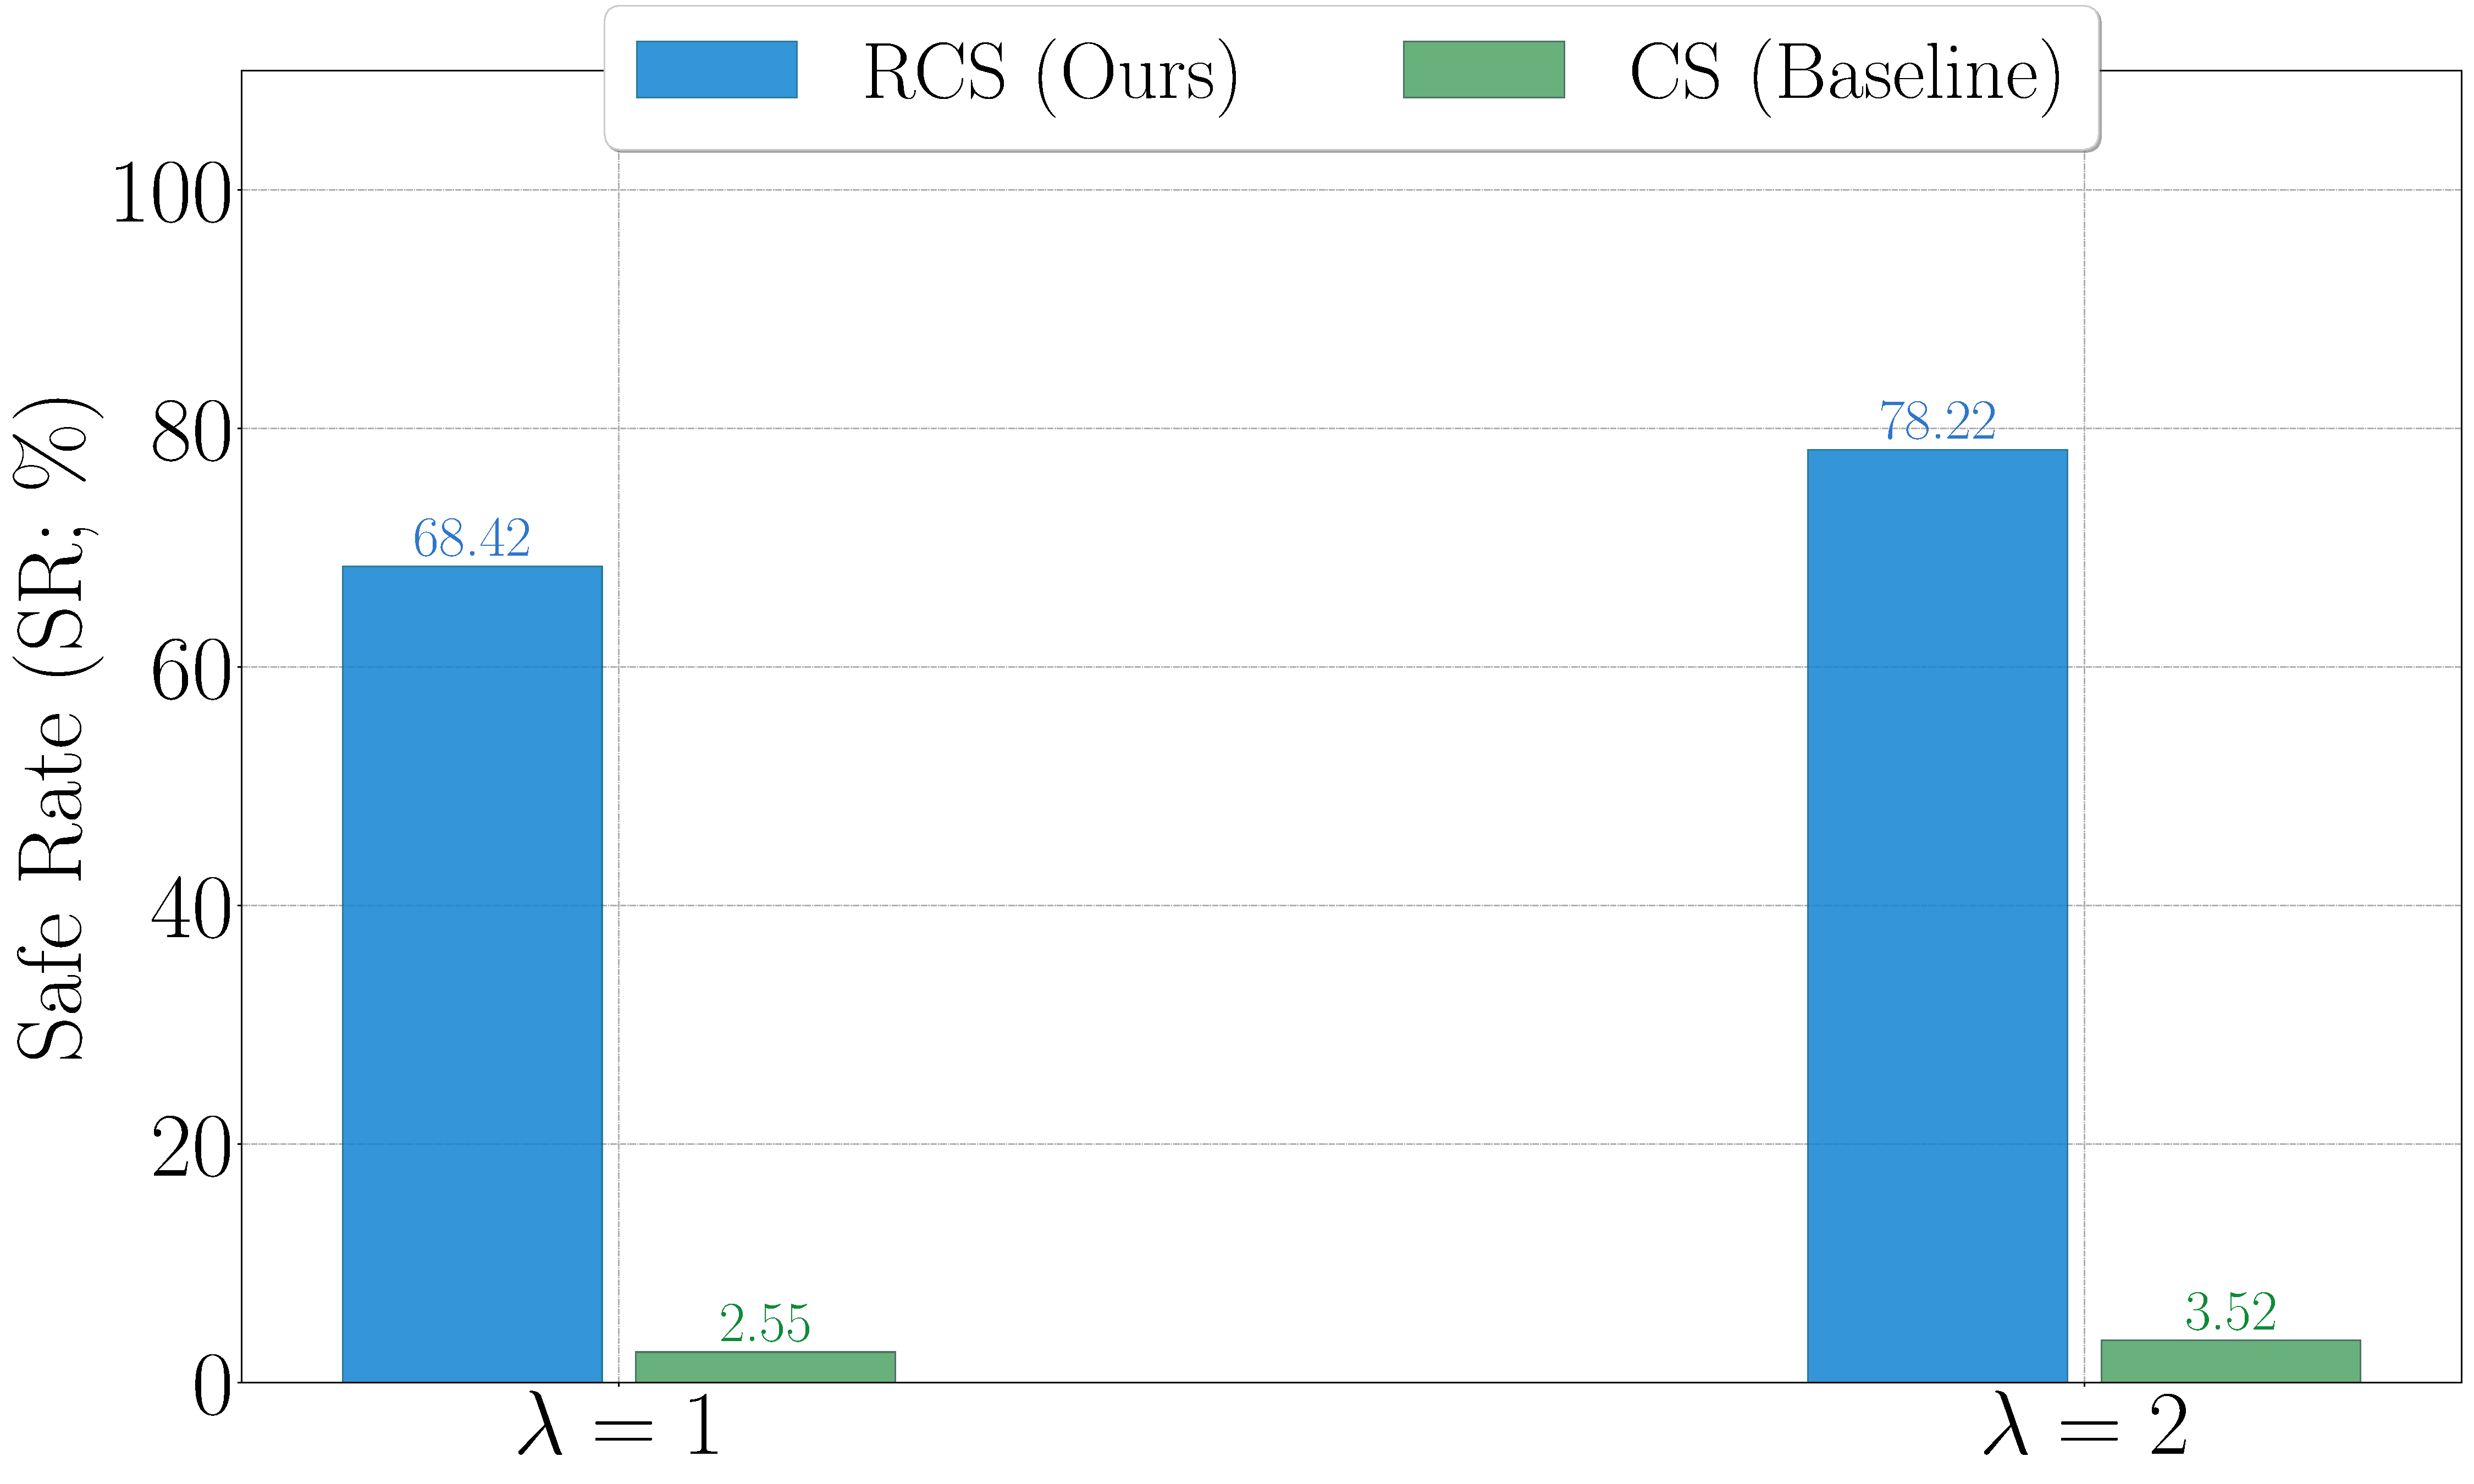
\includegraphics[width=\linewidth]{latex/eval_res_m/SR-5-m.pdf}
        \caption{$n=5$.}
    \end{subfigure}
    \begin{subfigure}{0.31\textwidth}
        \centering
        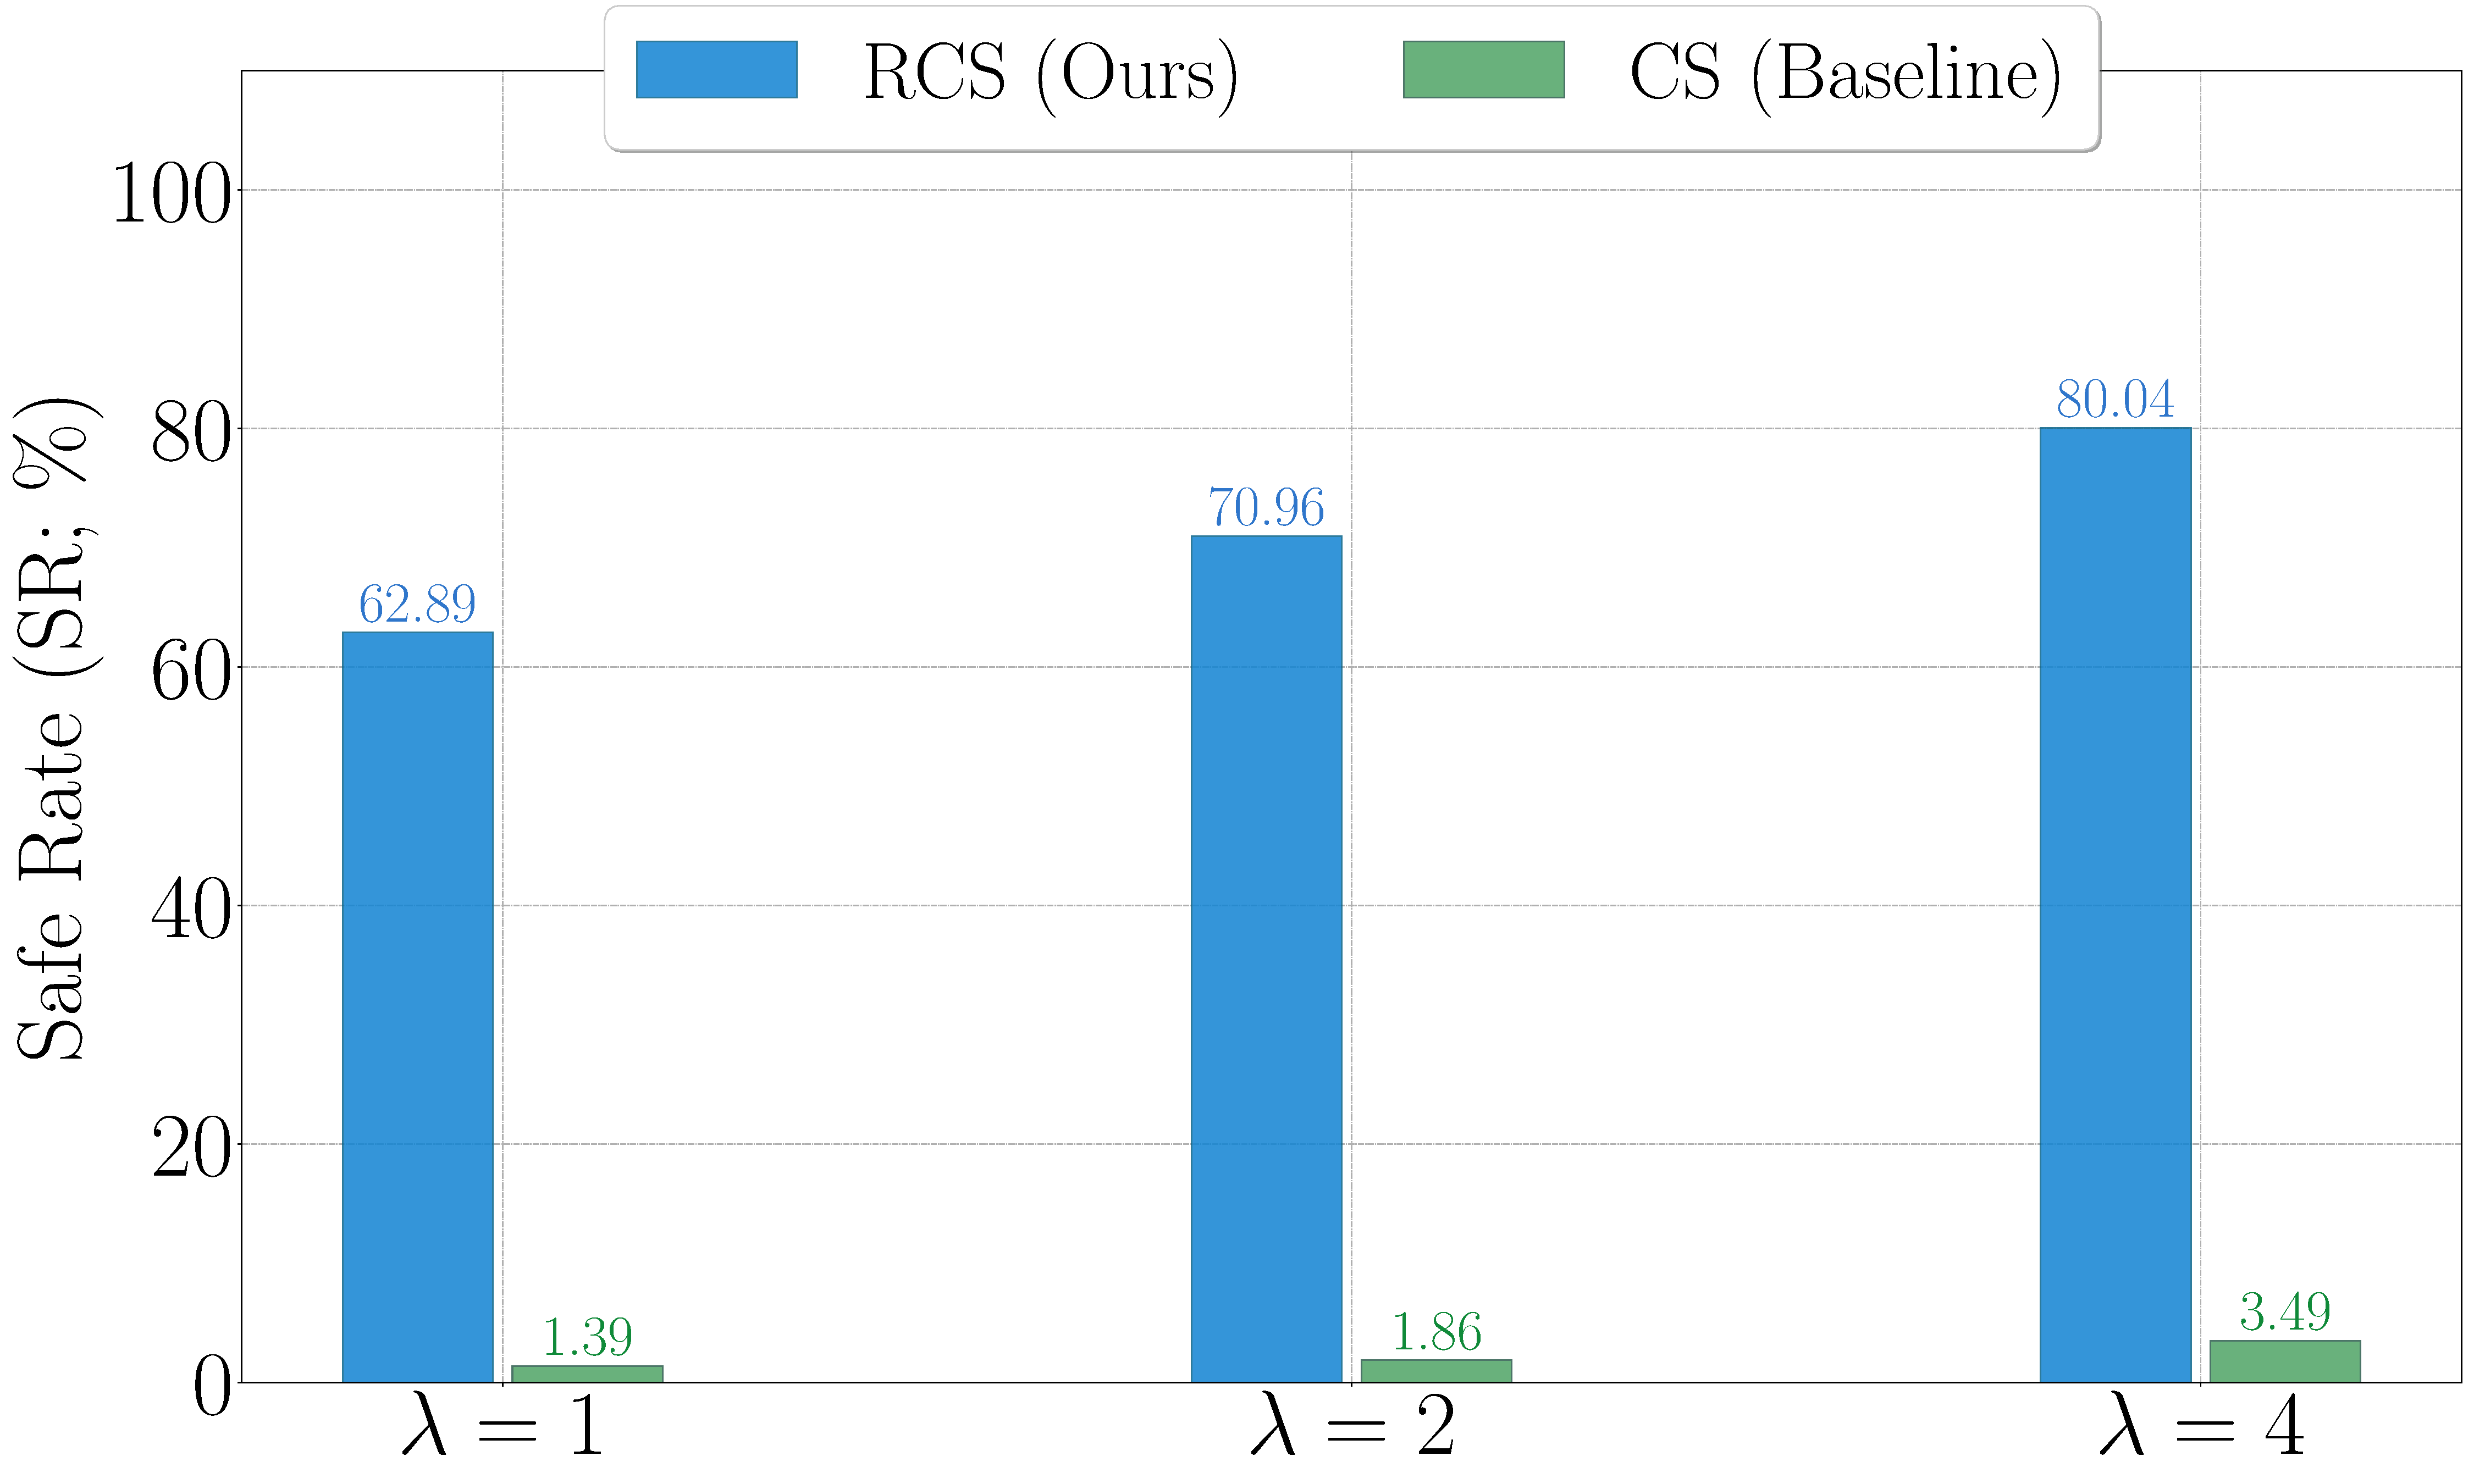
\includegraphics[width=\linewidth]{latex/eval_res_m/SR-9-m.pdf}
        \caption{$n=9$.}
    \end{subfigure}
    \begin{subfigure}{0.31\textwidth}
        \centering
        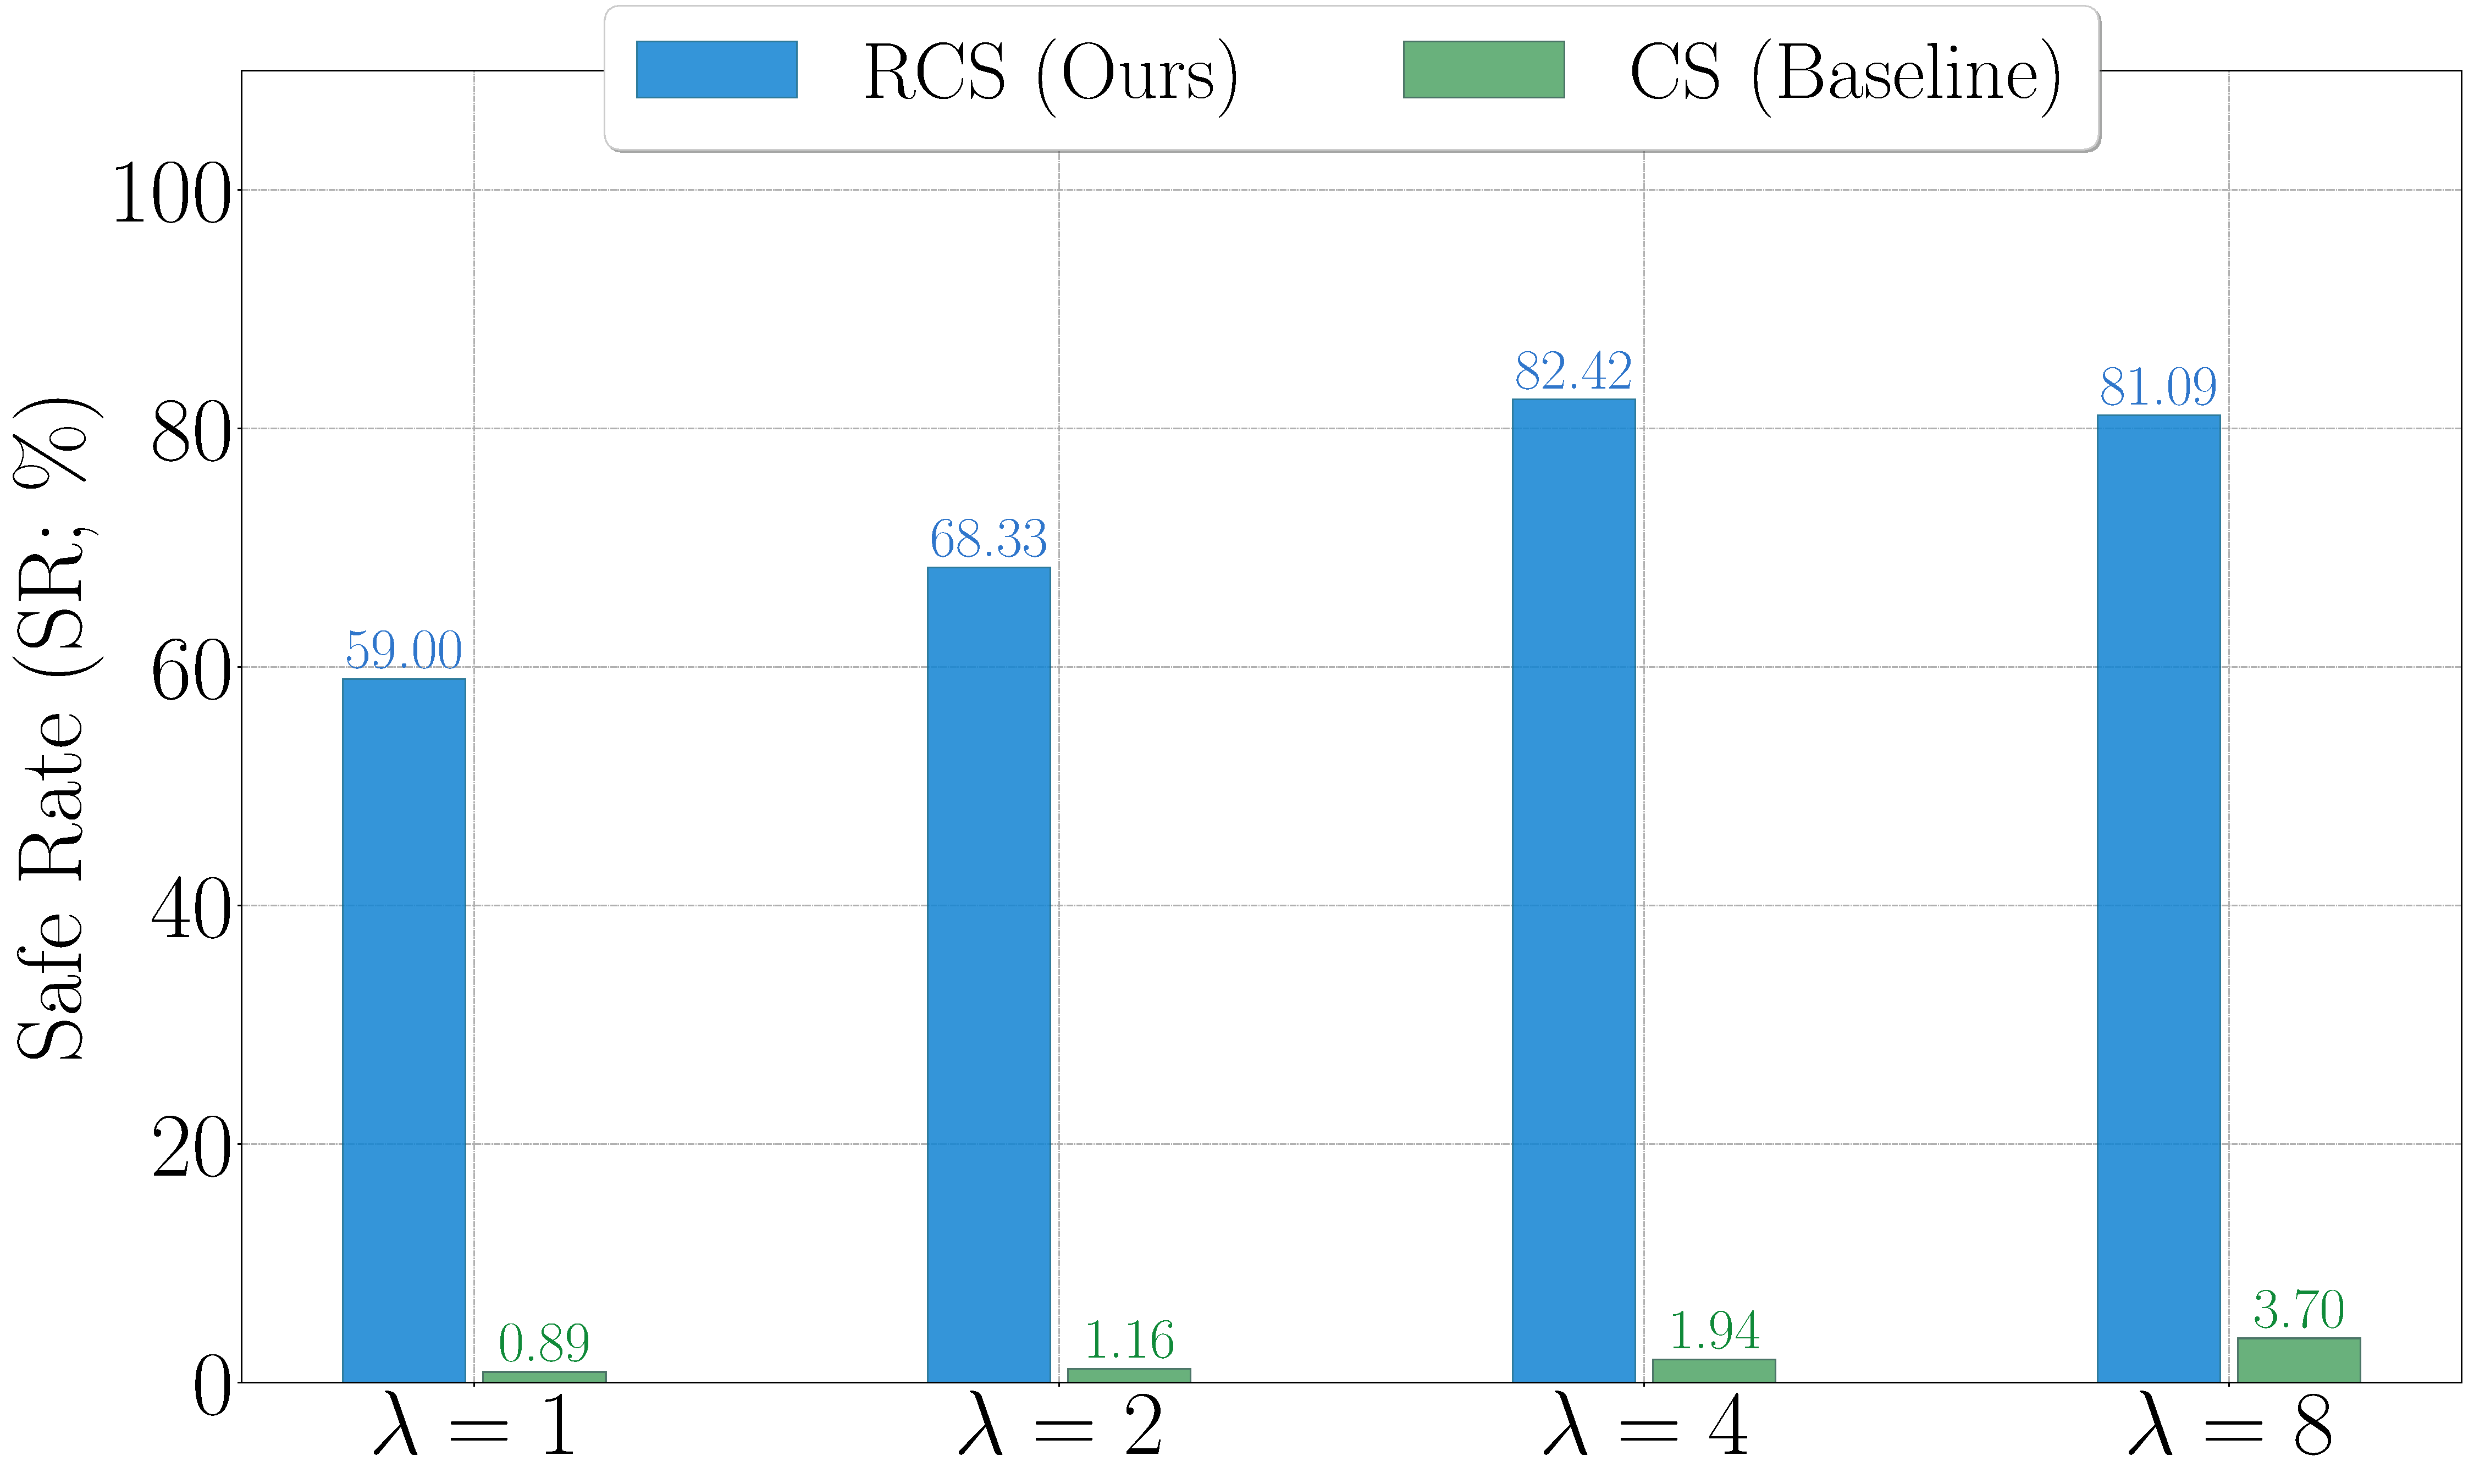
\includegraphics[width=\linewidth]{latex/eval_res_m/SR-17-m.pdf}
        \caption{$n=17$.}
    \end{subfigure}
    \caption{Evaluation results for the safe rate when Byzantine models collude.}
    \label{fig:sr_m_app}
    \vspace{-15pt}
\end{figure*}

\newpage
\begin{figure*}[!]
    \centering
    \begin{subfigure}{0.32\textwidth}
        \centering
        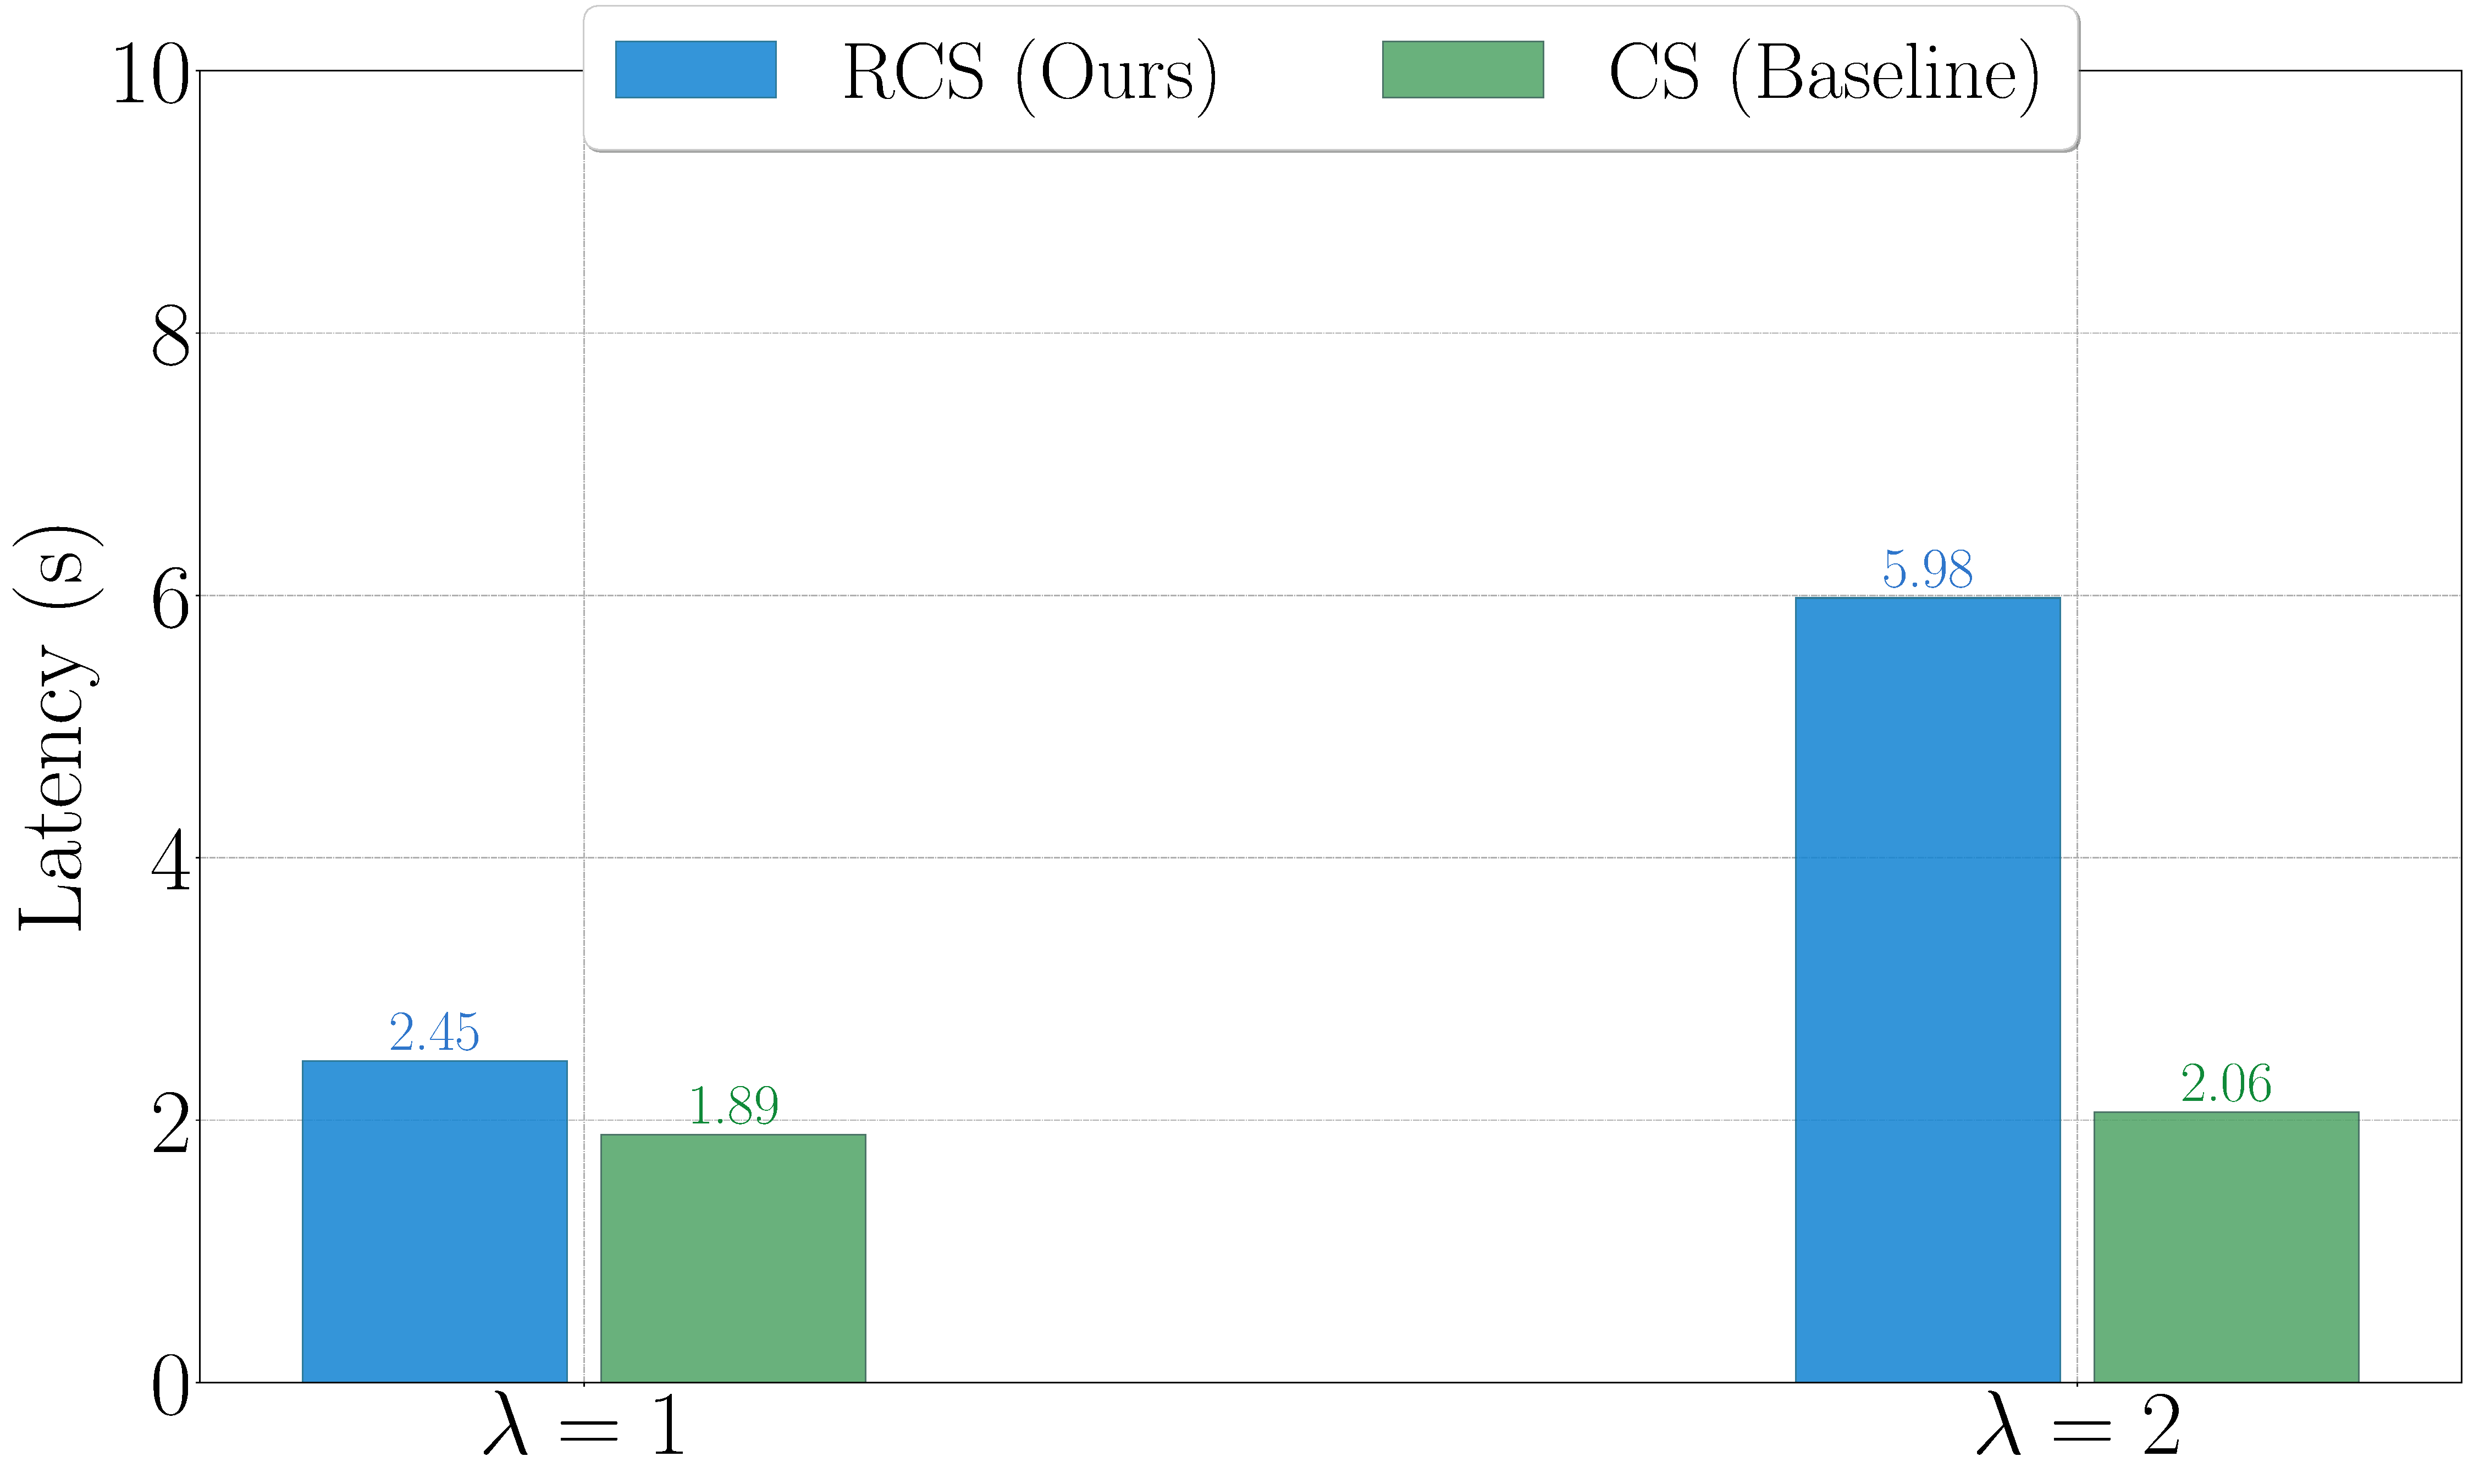
\includegraphics[width=\linewidth]{latex/eval_res_m/TC-5-m.pdf}
        \caption{$n=5$.}
    \end{subfigure}
    \begin{subfigure}{0.32\textwidth}
        \centering
        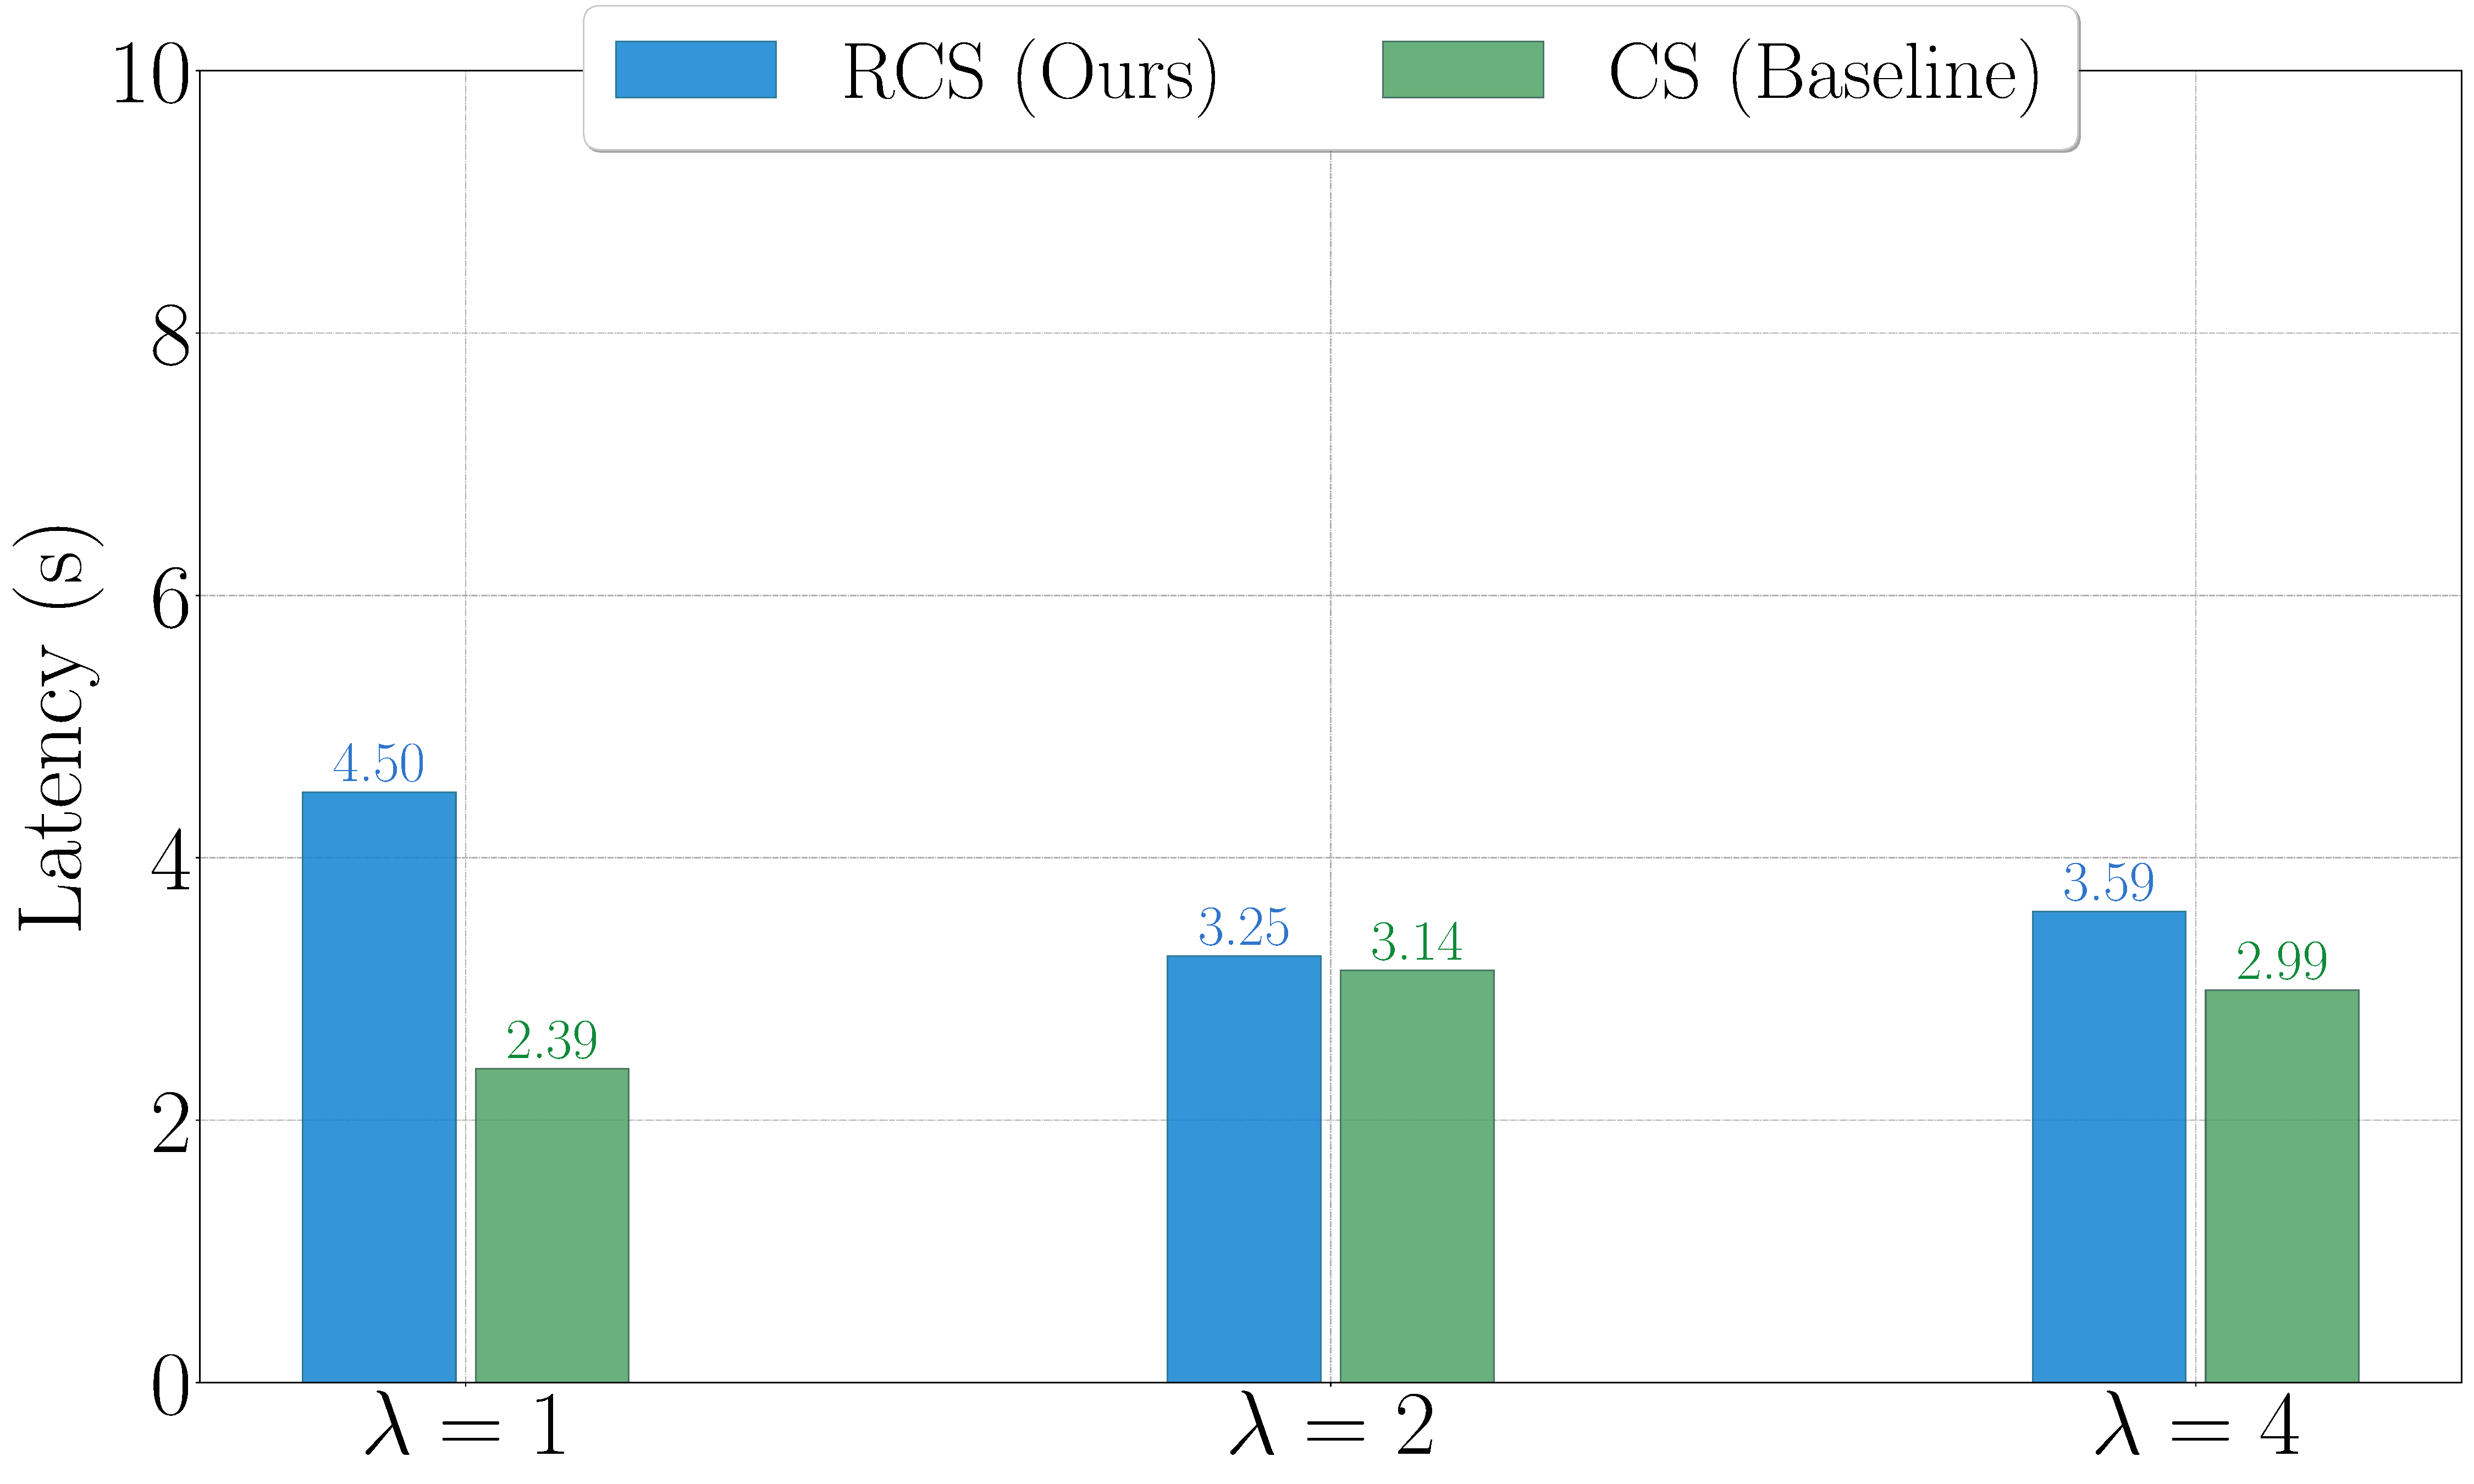
\includegraphics[width=\linewidth]{latex/eval_res_m/TC-9-m.pdf}
        \caption{$n=9$.}
    \end{subfigure}
    \begin{subfigure}{0.32\textwidth}
        \centering
        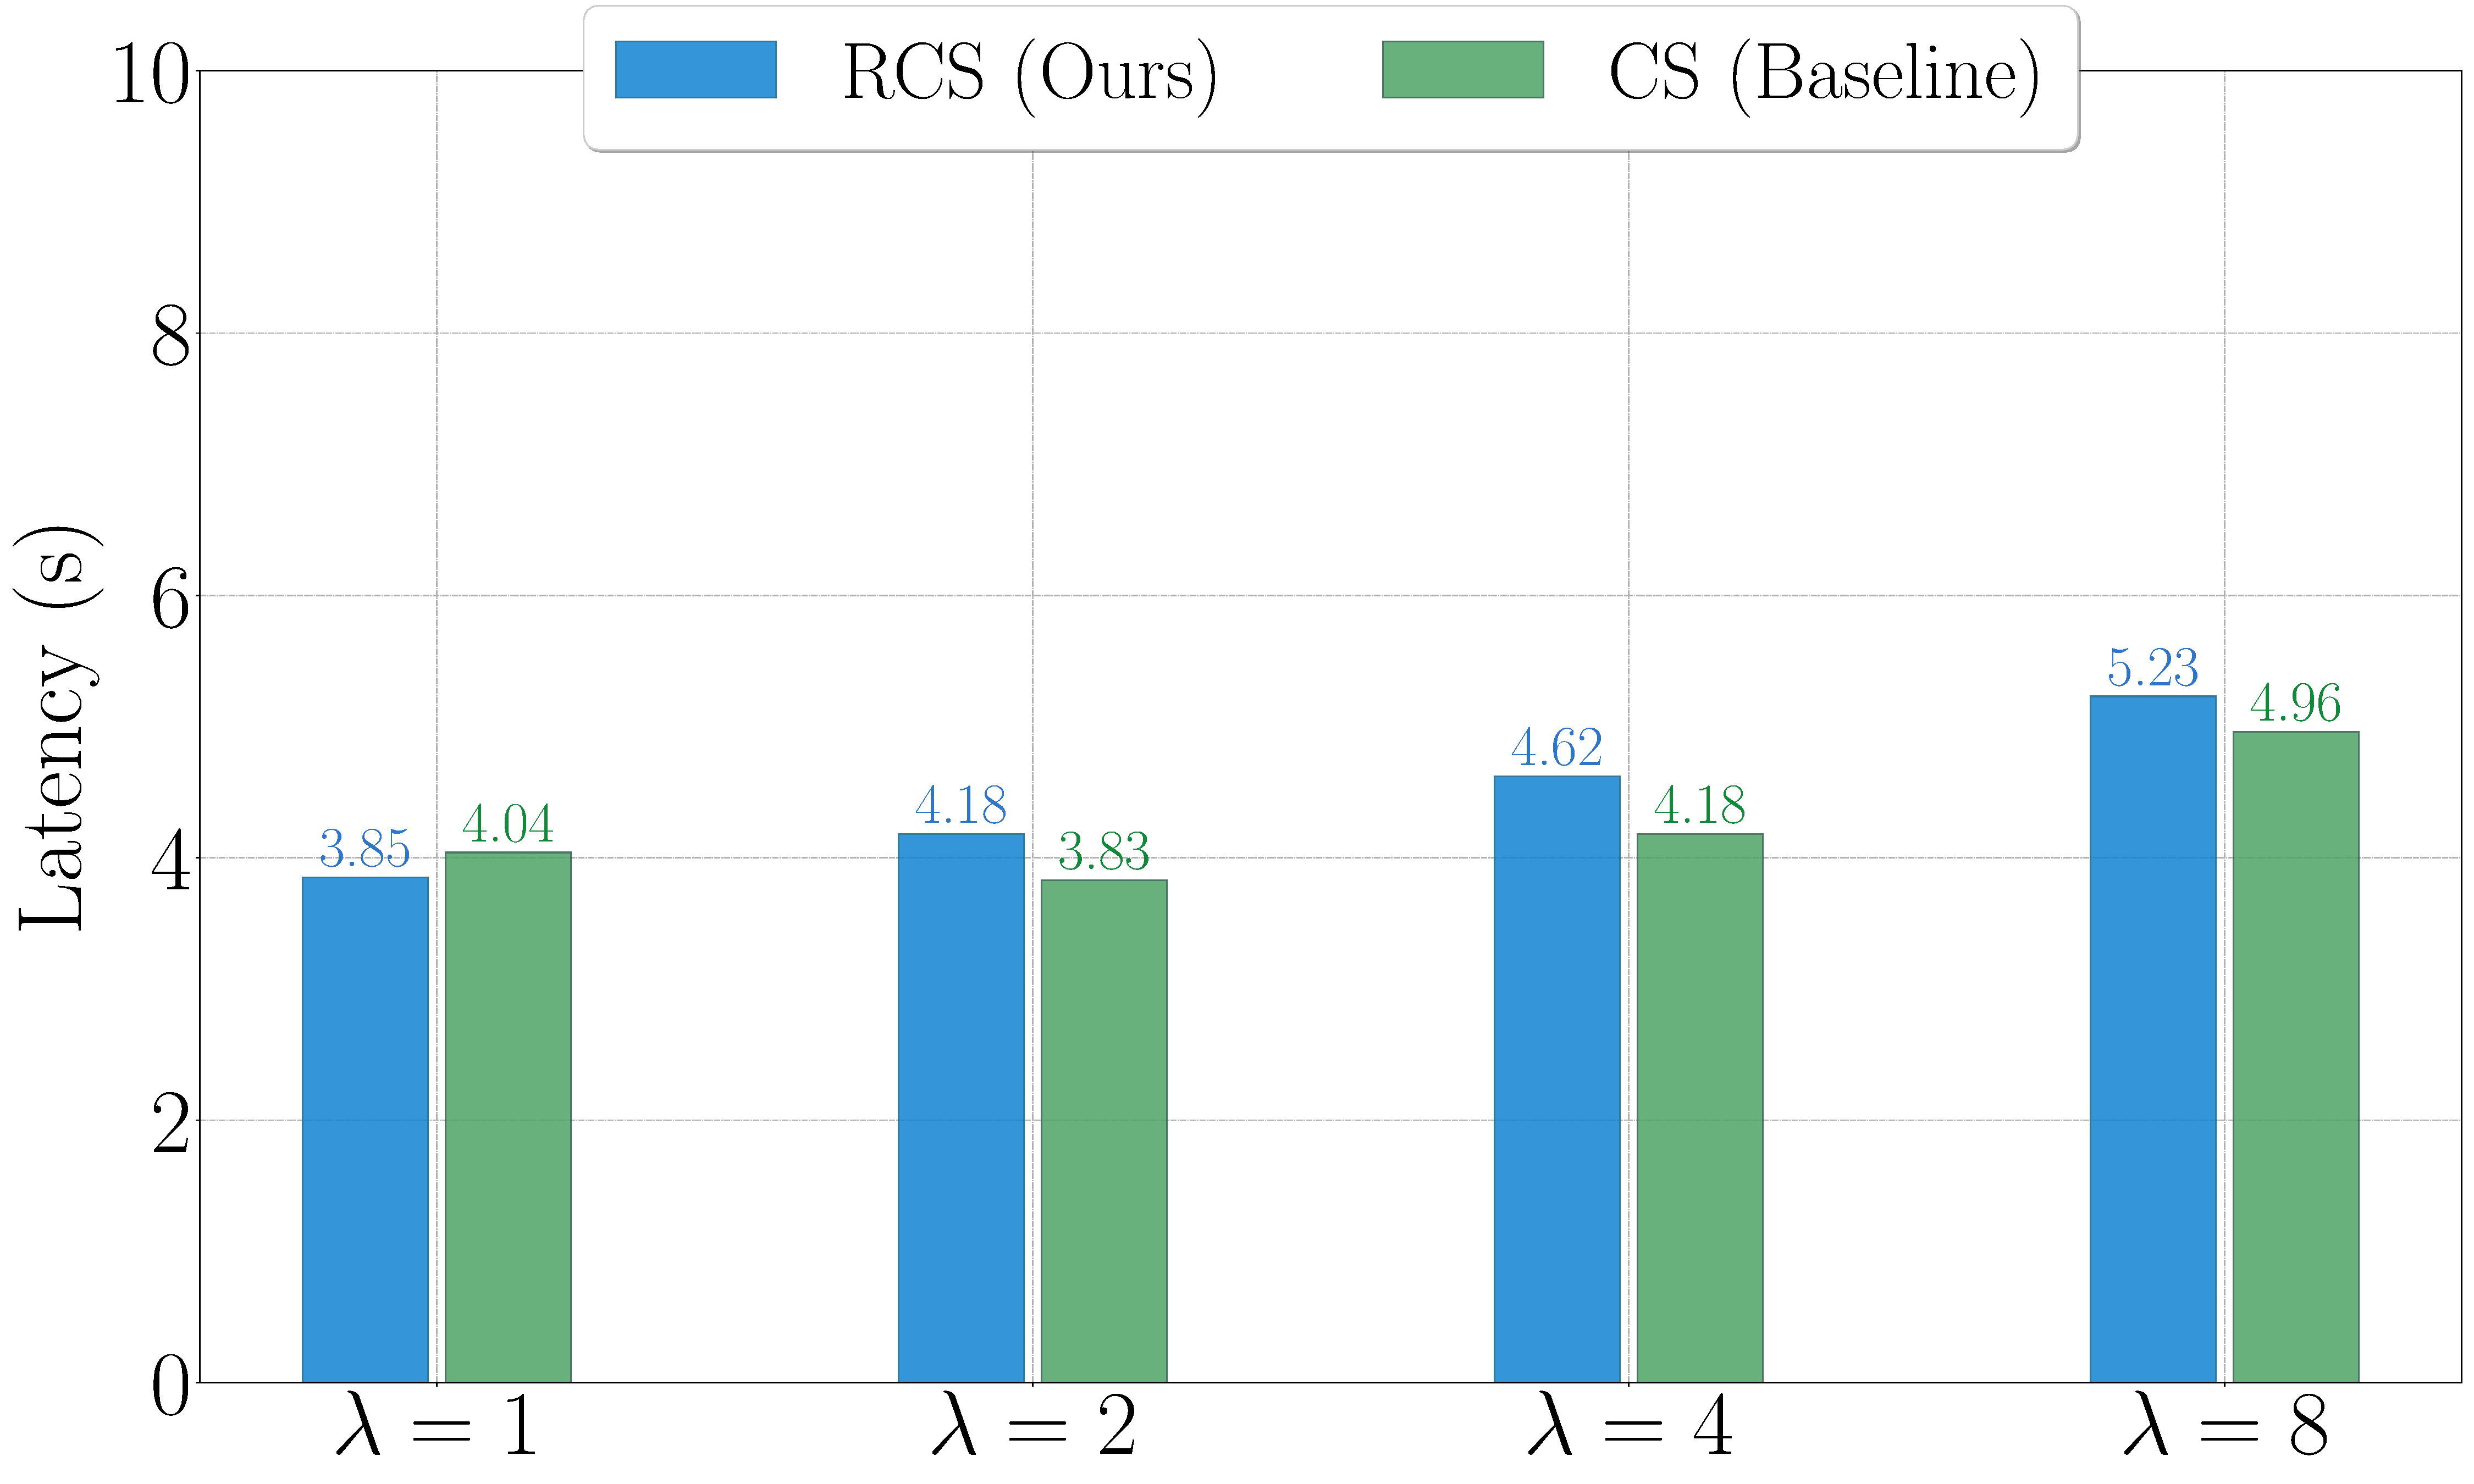
\includegraphics[width=\linewidth]{latex/eval_res_m/TC-17-m.pdf}
        \caption{$n=17$.}
    \end{subfigure}
    \caption{Evaluation results for the latency when Byzantine models collude.}
    \label{fig:TC_m_app}
    % \vspace{-15pt}
\end{figure*}

\begin{figure*}[!]
    \centering
    \begin{subfigure}{0.31\textwidth}
        \centering
        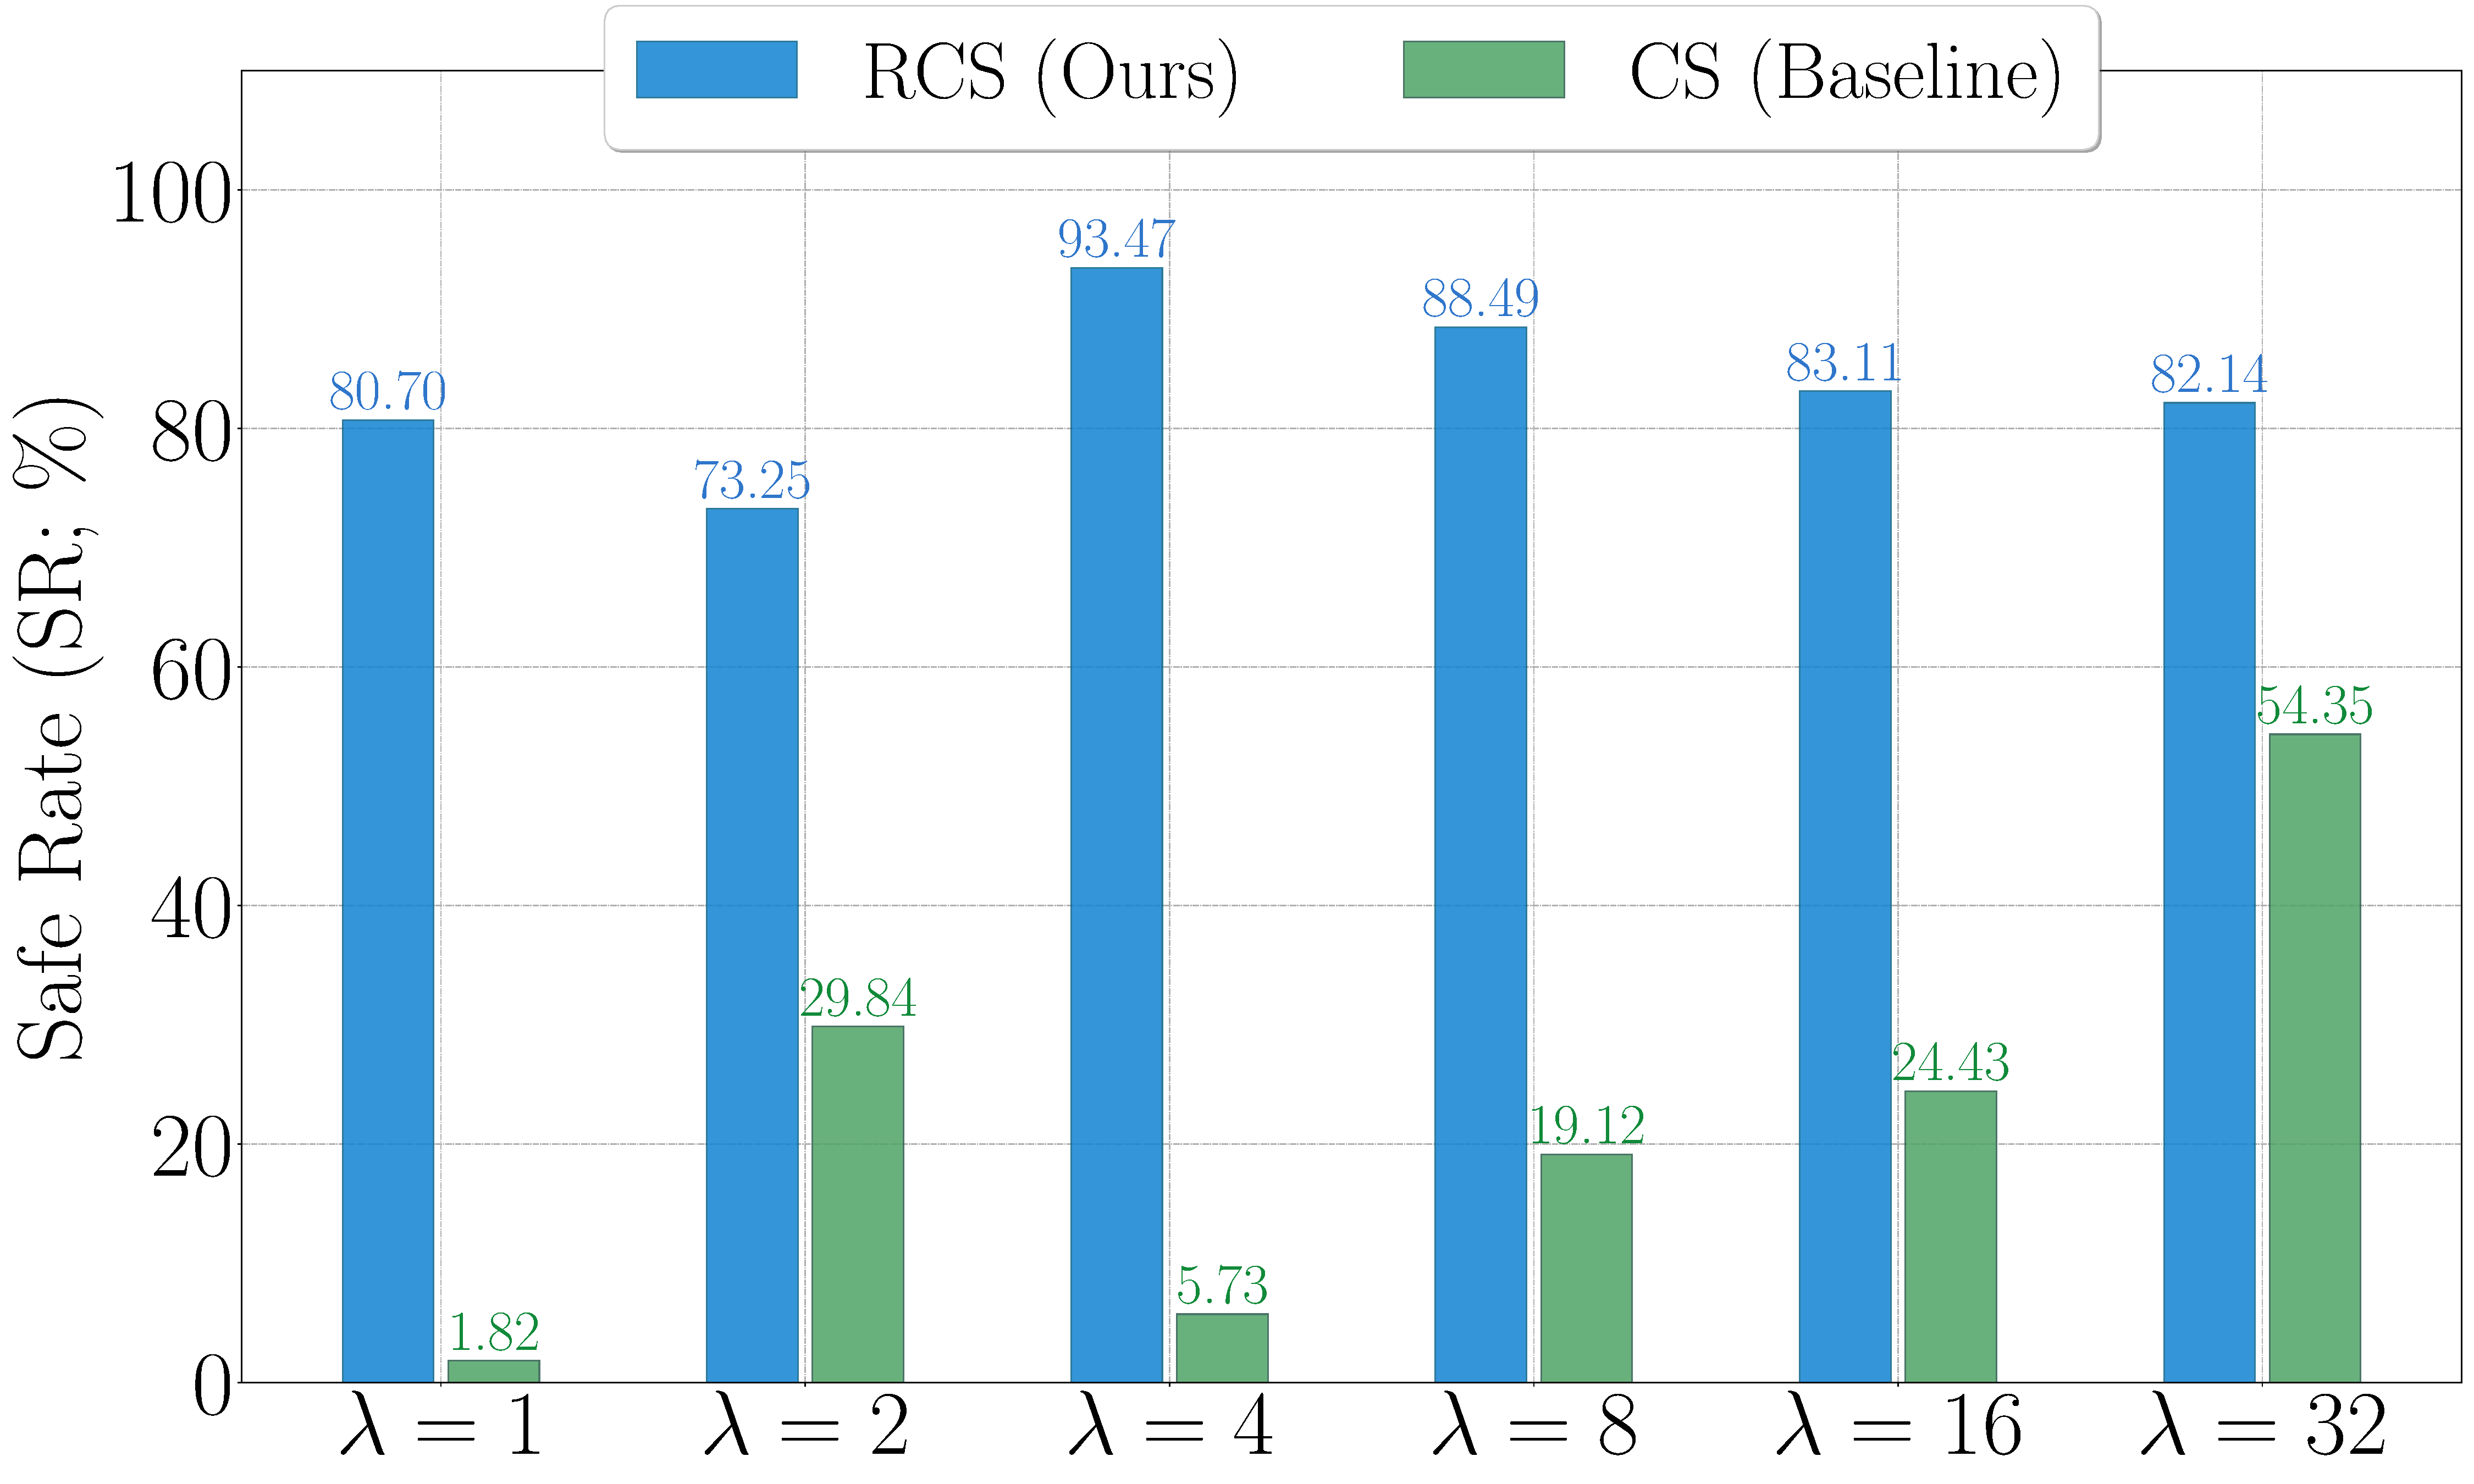
\includegraphics[width=\linewidth]{latex/eval_res_d/SR-34.pdf}
        \caption{$n=34$.}
    \end{subfigure}
    \begin{subfigure}{0.31\textwidth}
        \centering
        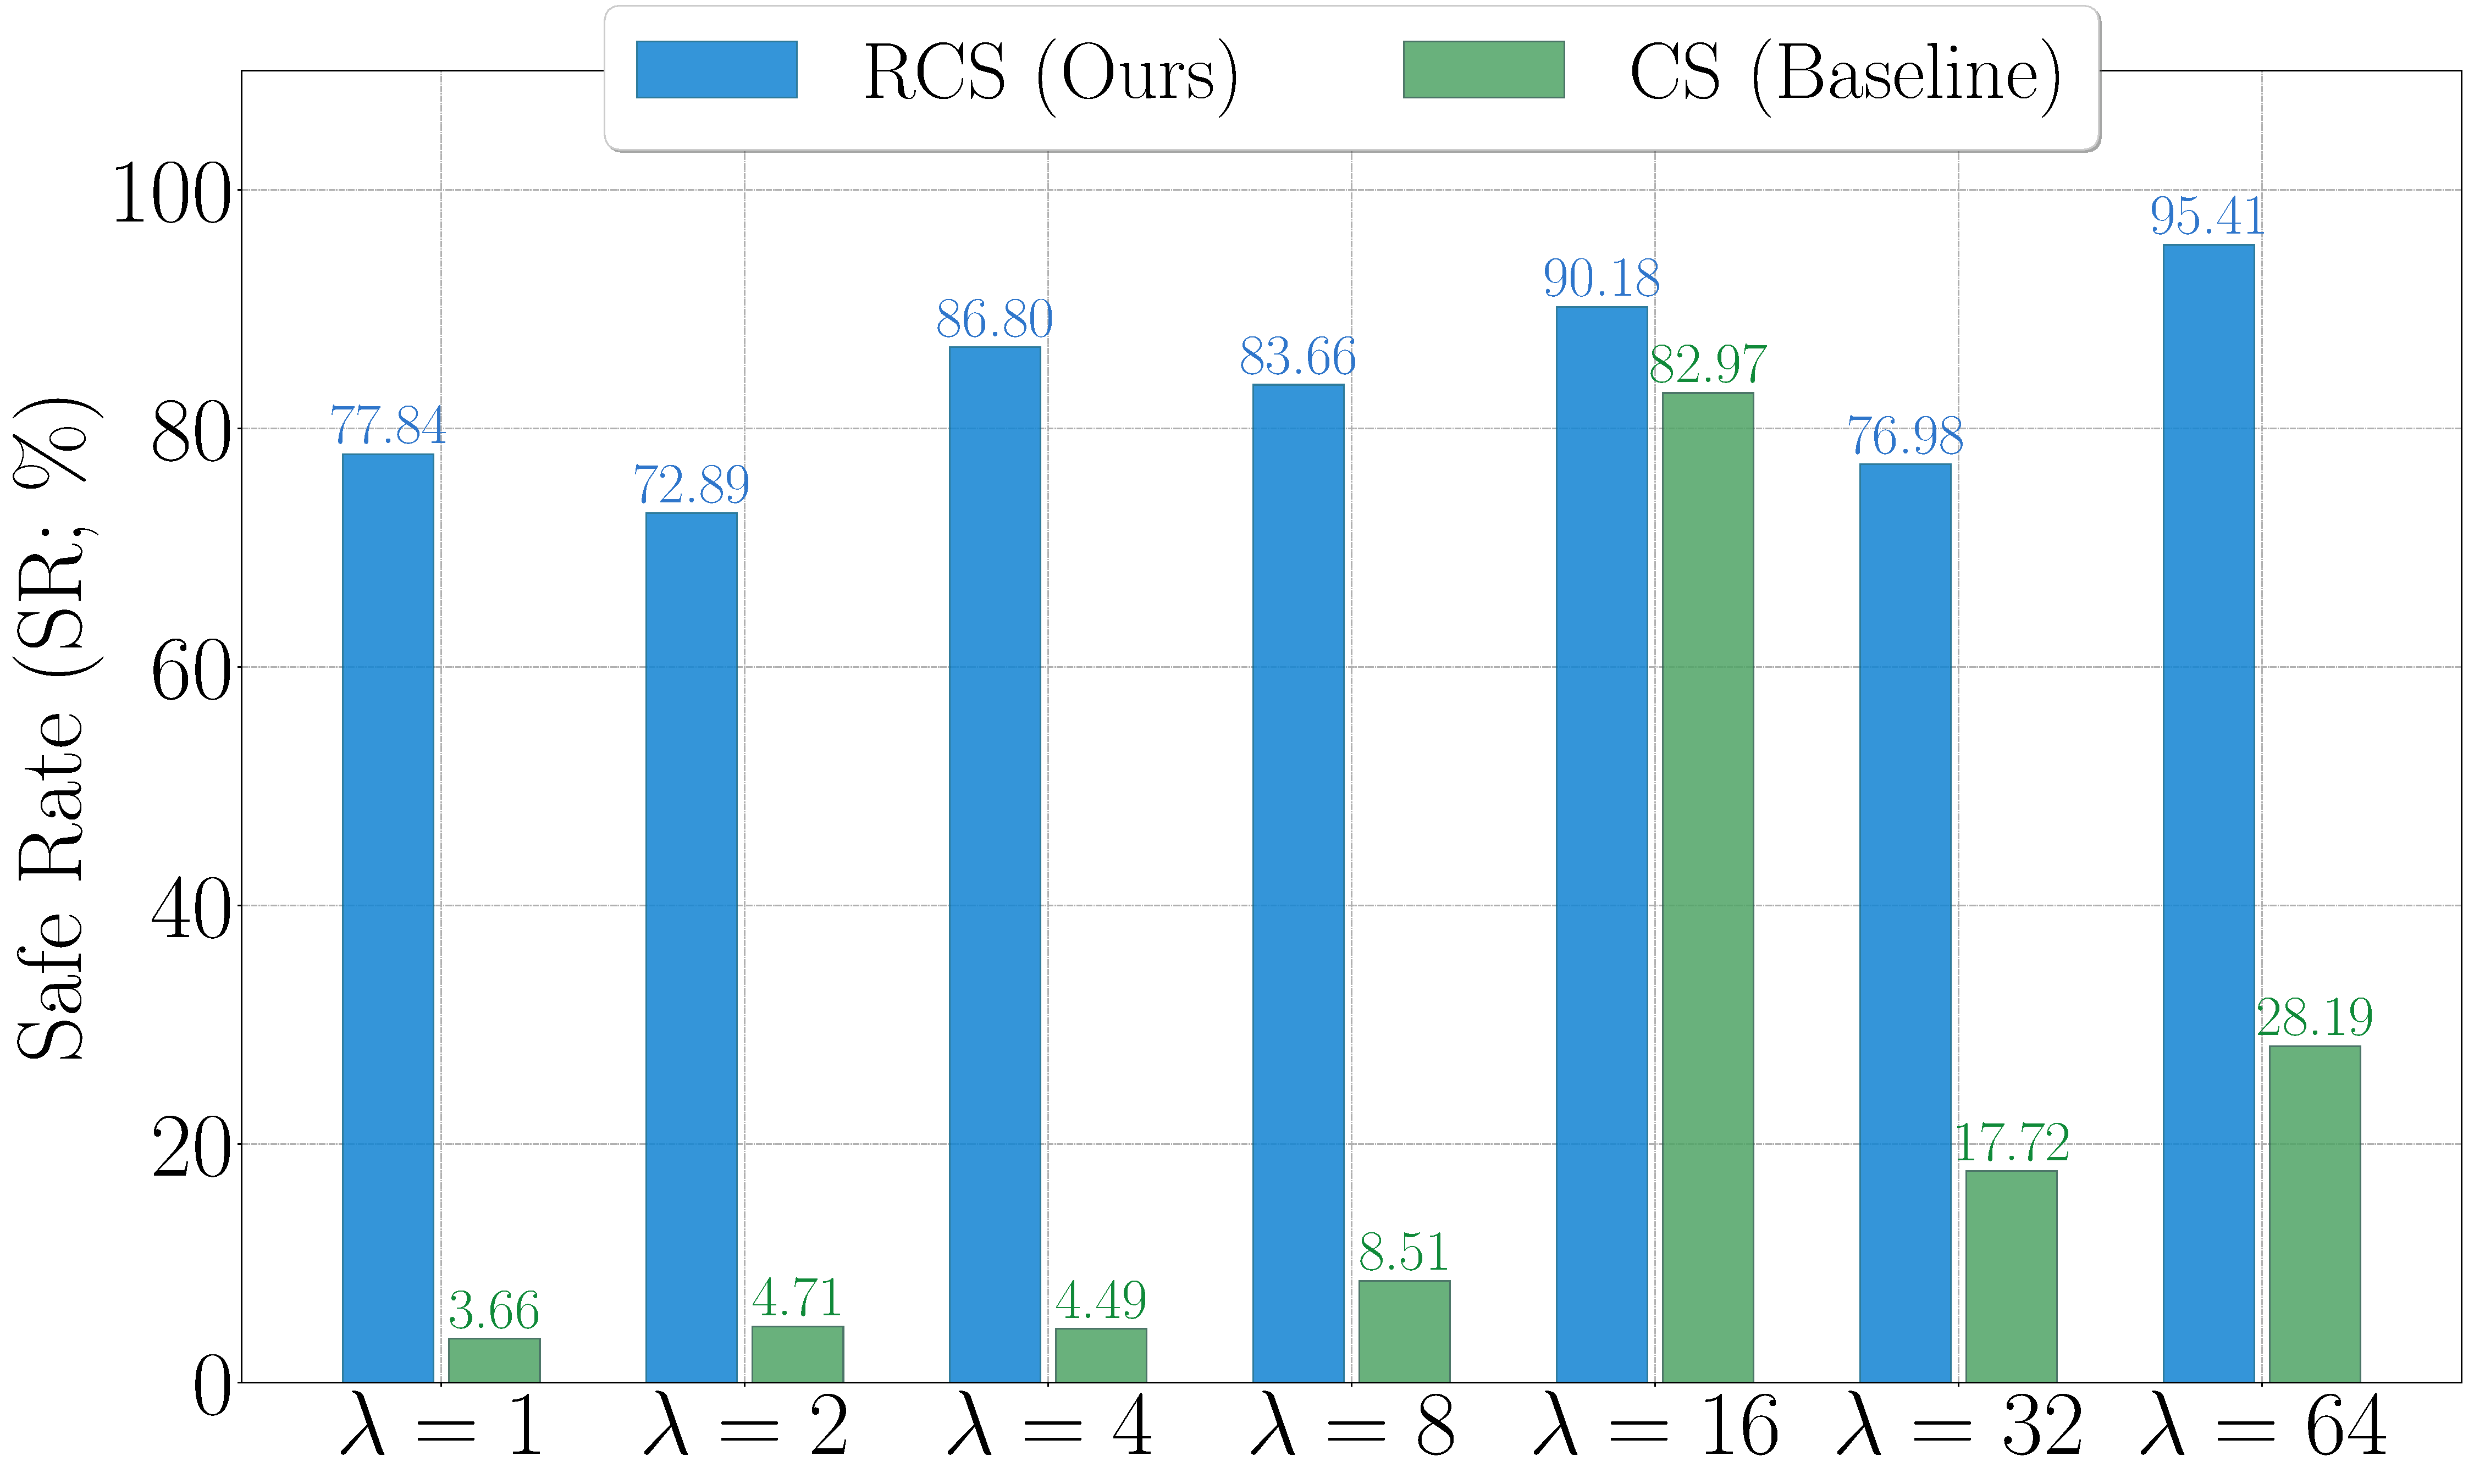
\includegraphics[width=\linewidth]{latex/eval_res_d/SR-66.pdf}
        \caption{$n=66$.}
    \end{subfigure}
    \begin{subfigure}{0.35\textwidth}
        \centering
        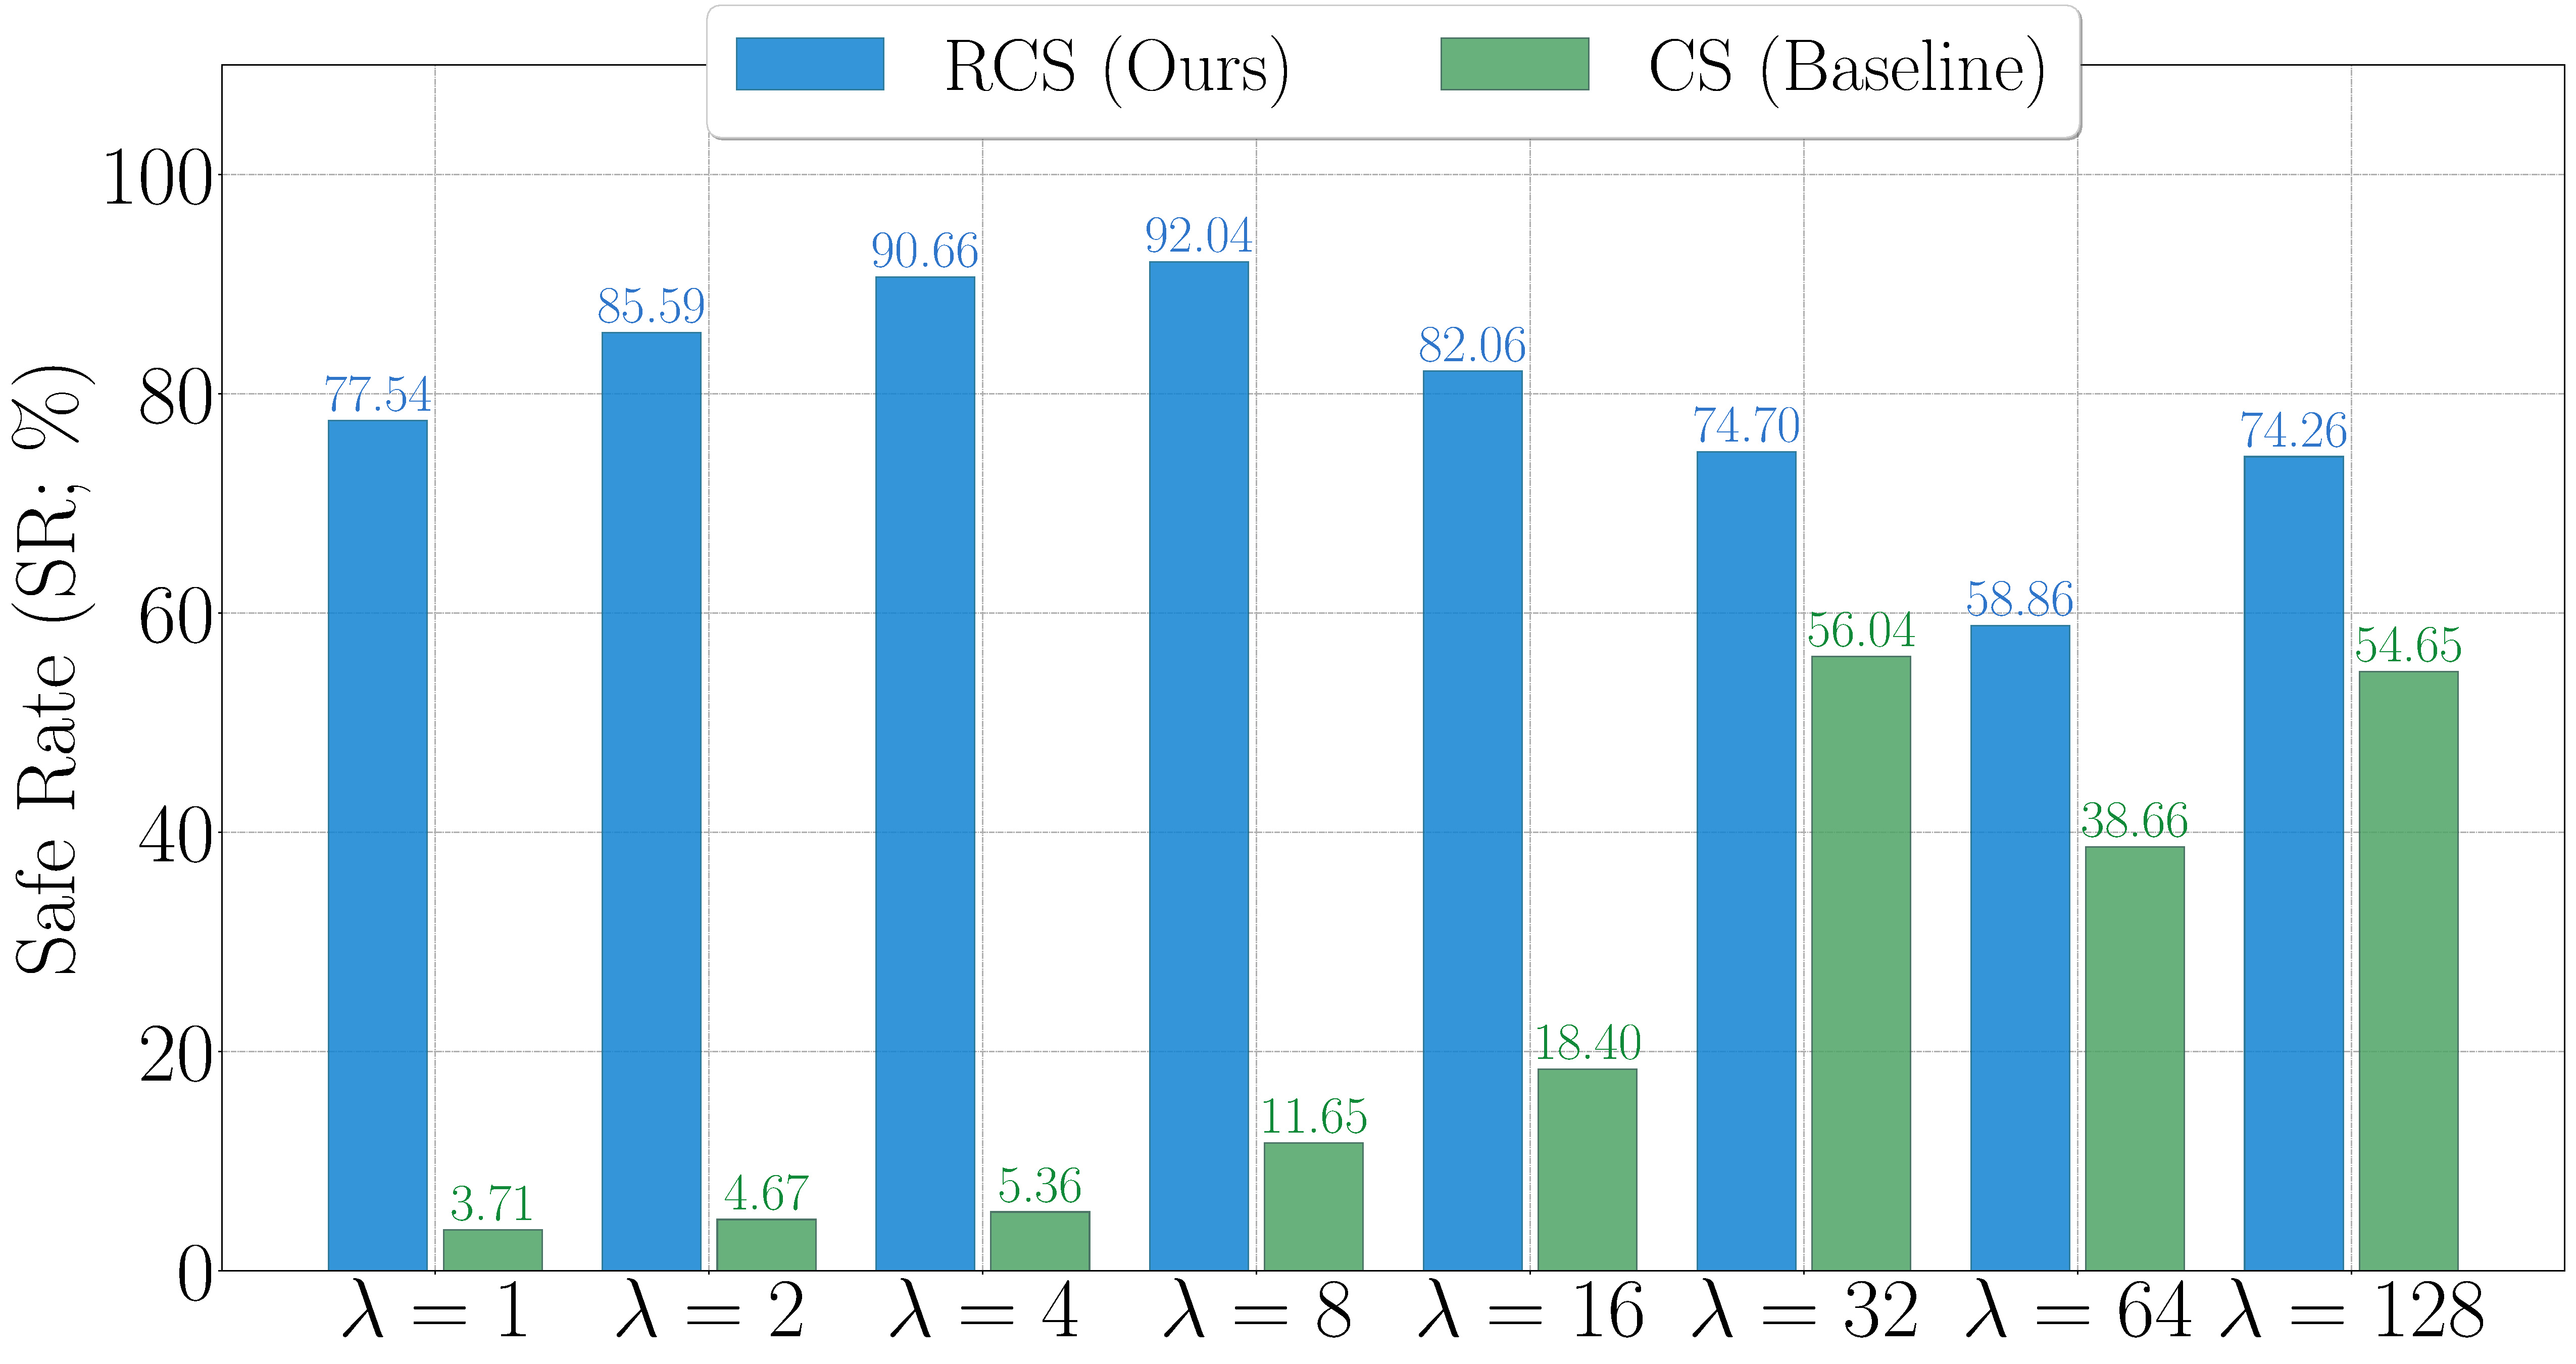
\includegraphics[width=\linewidth]{latex/eval_res_d/SR-130.pdf}
        \caption{$n=130$.}
    \end{subfigure}
    \caption{Evaluation results for the safe rate when $f = \lceil \frac{n}{2} \rceil$.}
    \label{fig:SR_d_app}
    % \vspace{-15pt}
\end{figure*}



\begin{figure*}[!]
    \centering
    \begin{subfigure}{0.31\textwidth}
        \centering
        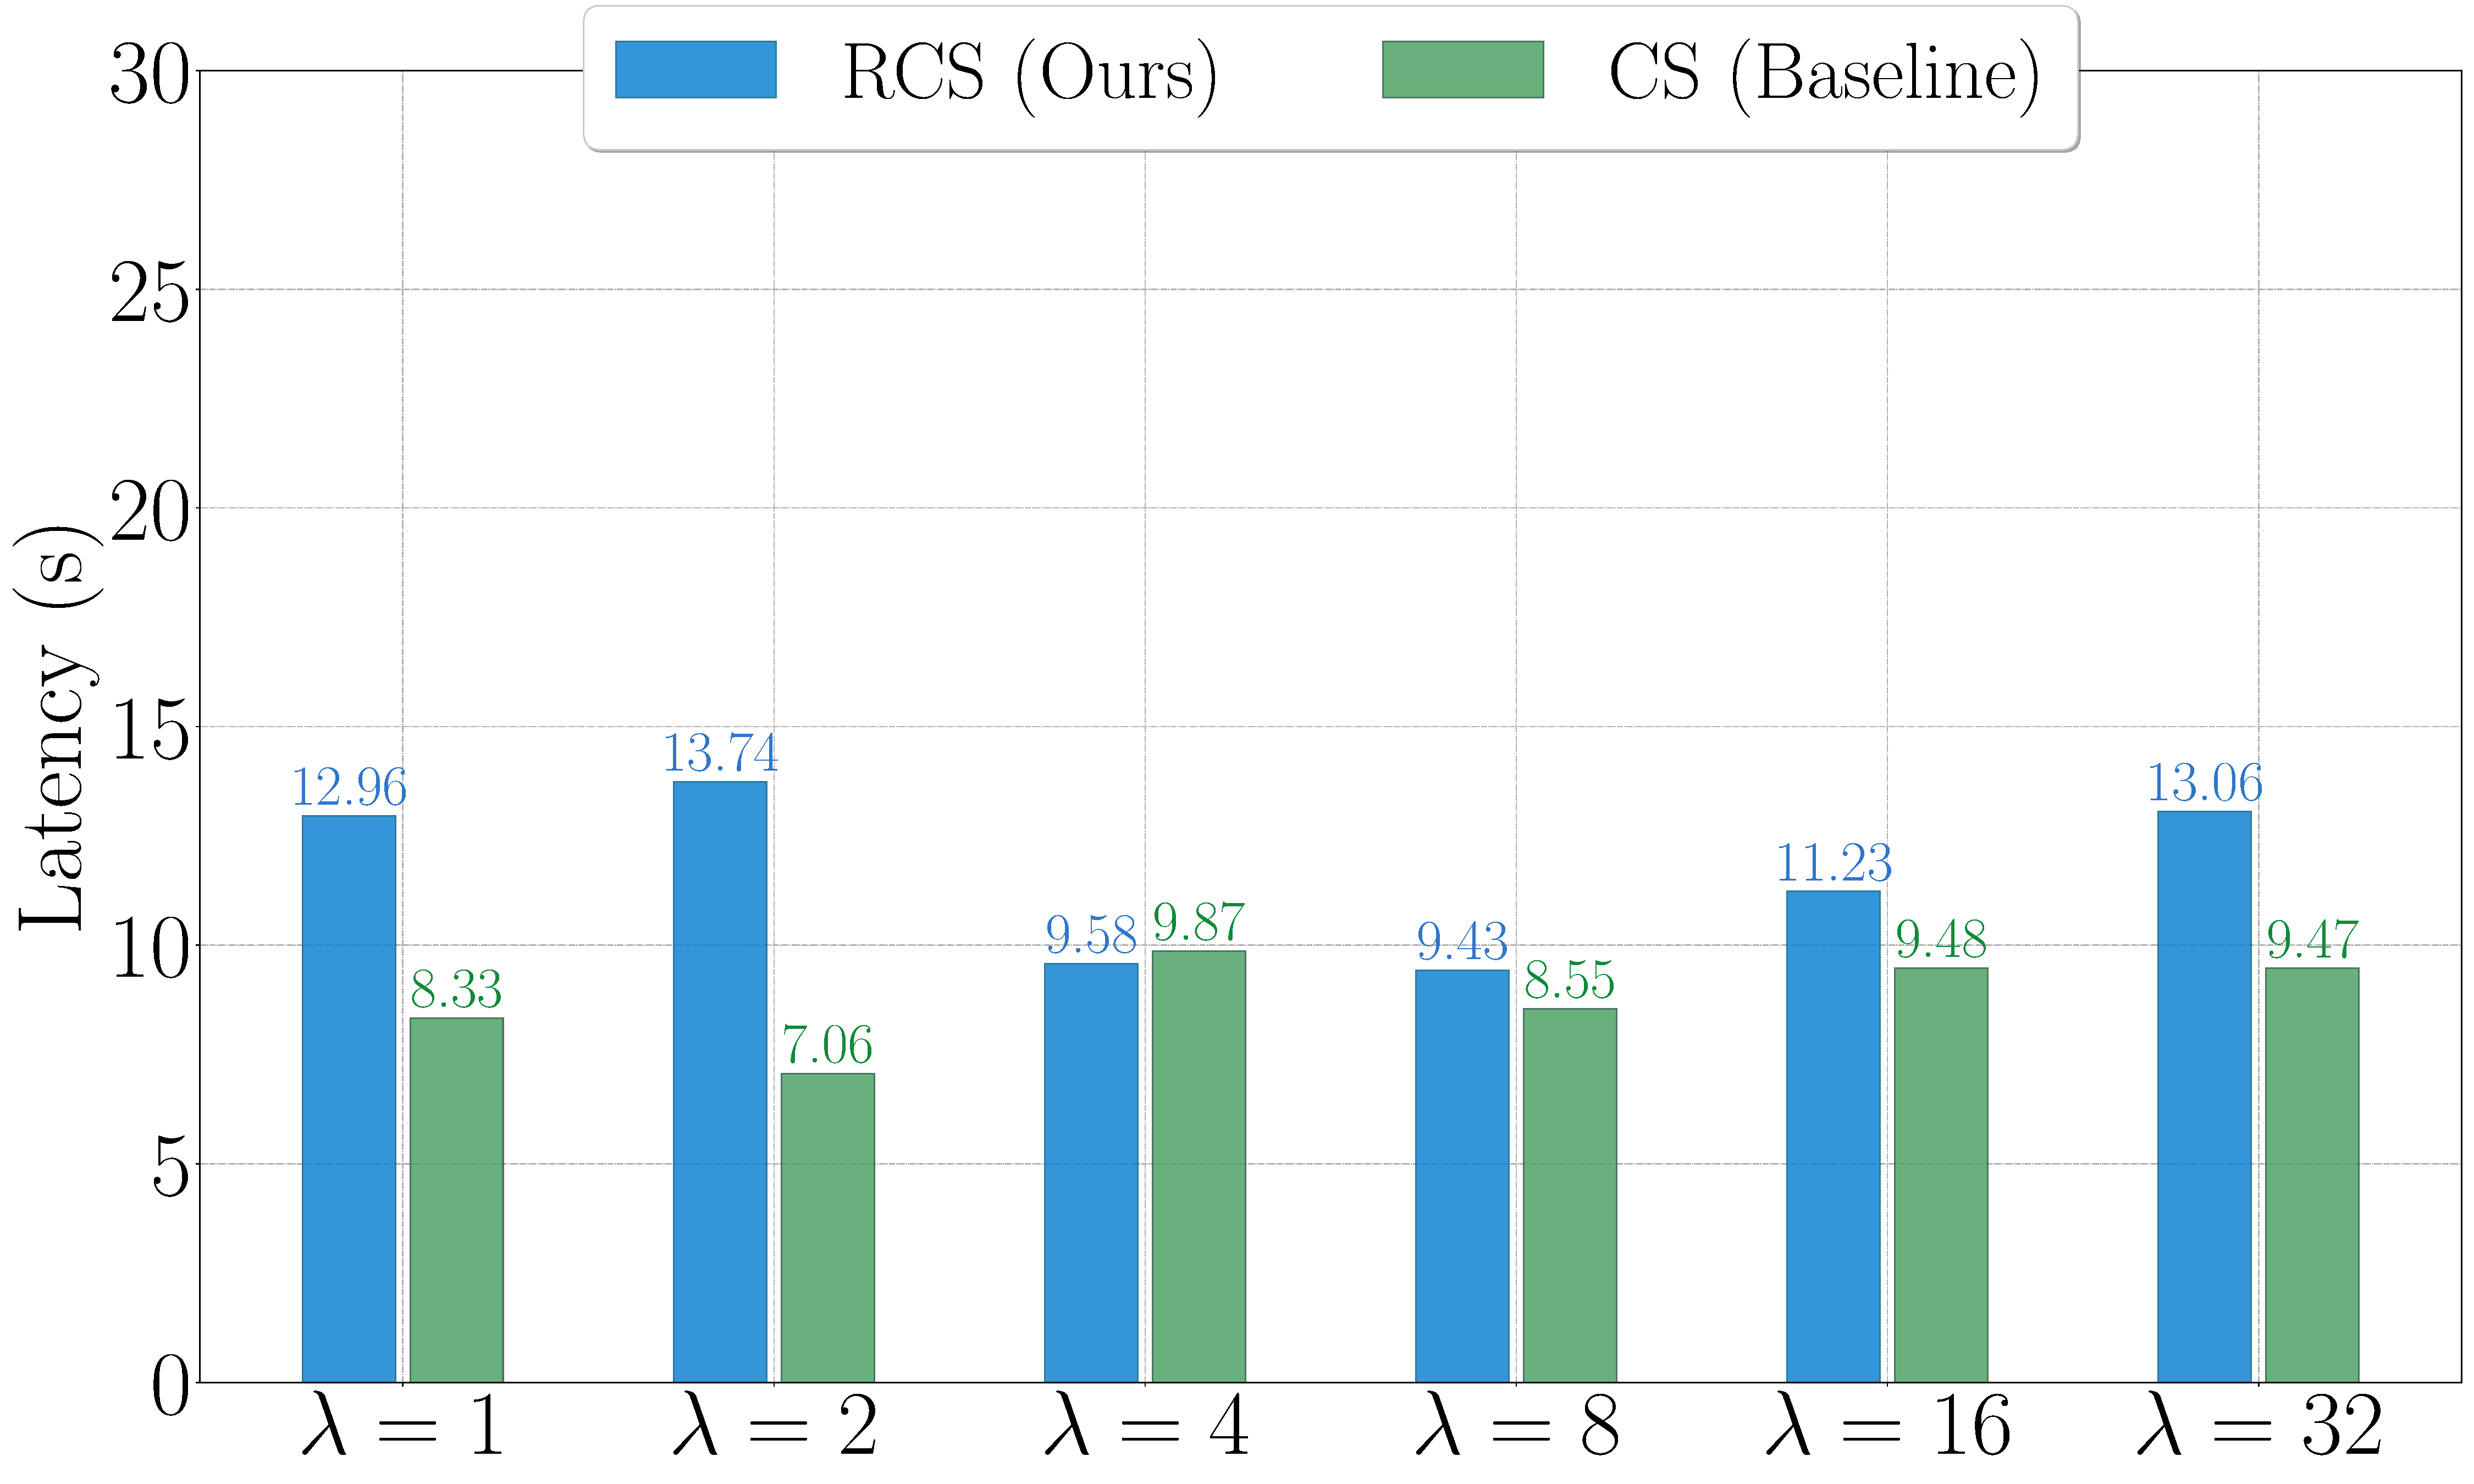
\includegraphics[width=\linewidth]{latex/eval_res_d/TC-34.pdf}
        \caption{$n=34$.}
    \end{subfigure}
    \begin{subfigure}{0.31\textwidth}
        \centering
        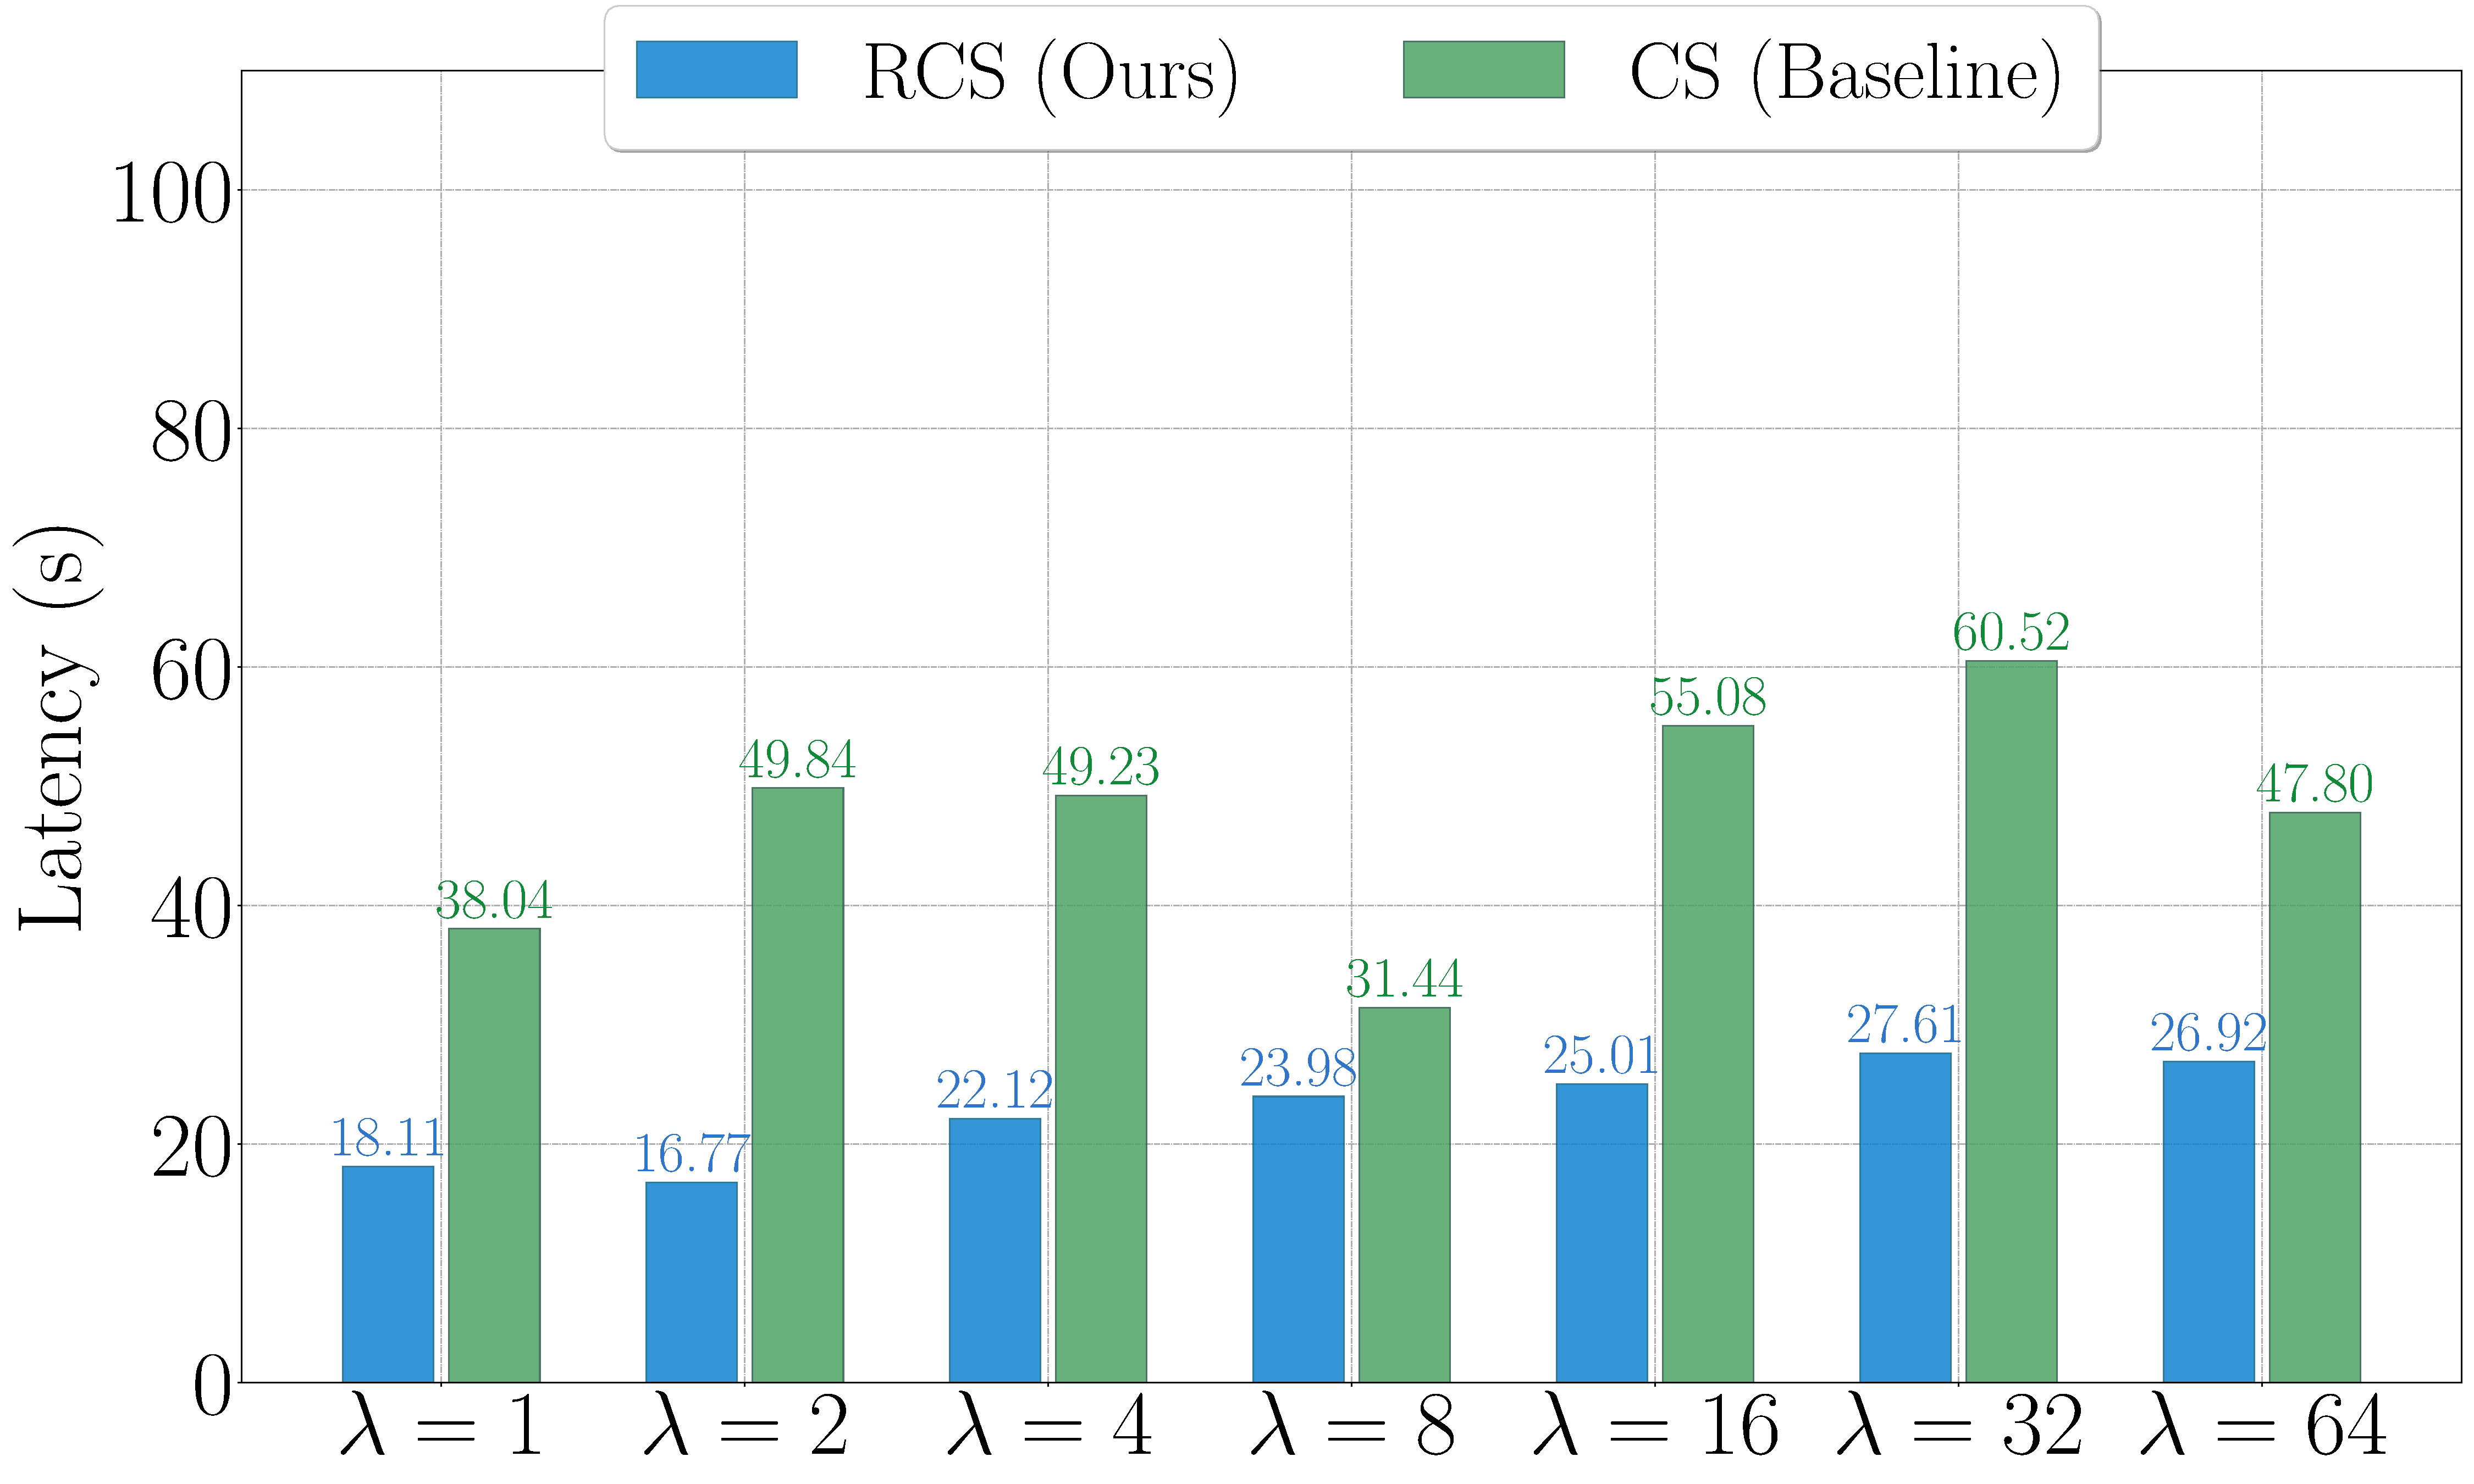
\includegraphics[width=\linewidth]{latex/eval_res_d/TC-66.pdf}
        \caption{$n=66$.}
    \end{subfigure}
    \begin{subfigure}{0.35\textwidth}
        \centering
        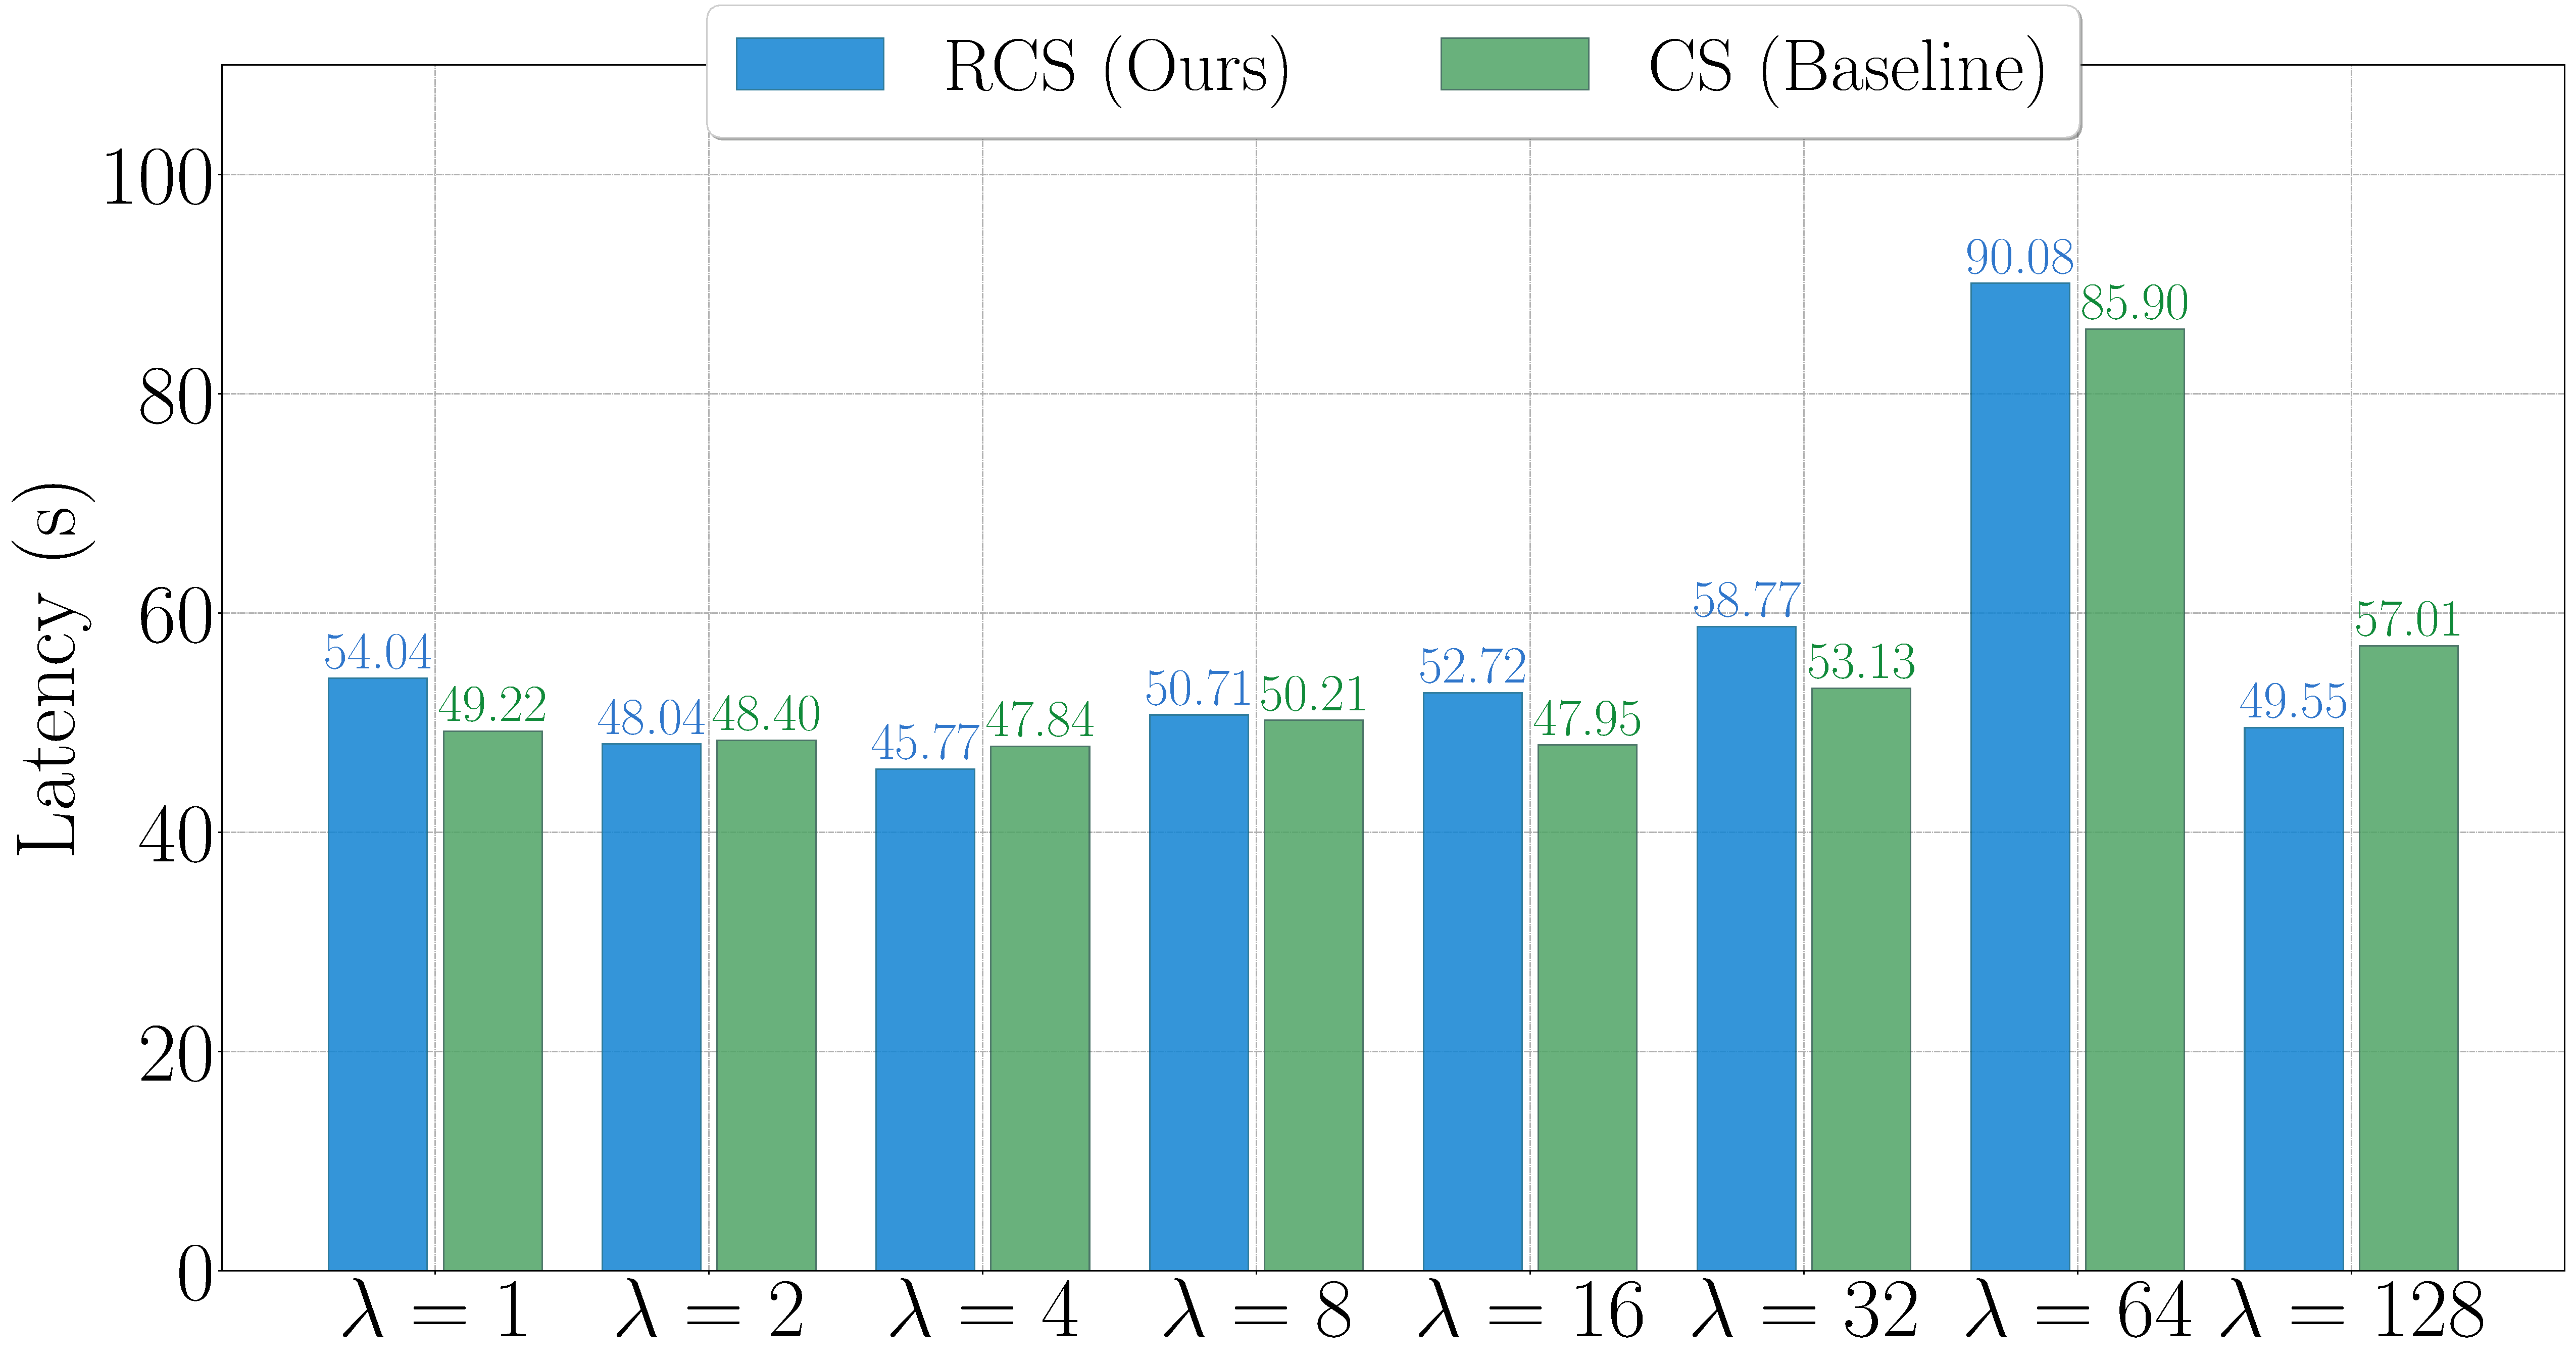
\includegraphics[width=\linewidth]{latex/eval_res_d/TC-130.pdf}
        \caption{$n=130$.}
    \end{subfigure}
    \caption{Evaluation results for the latency when $f = \lceil \frac{n}{2} \rceil$.}
    \label{fig:TC_d_app}
    % \vspace{-15pt}
\end{figure*}

\begin{figure}[!]
    \centering
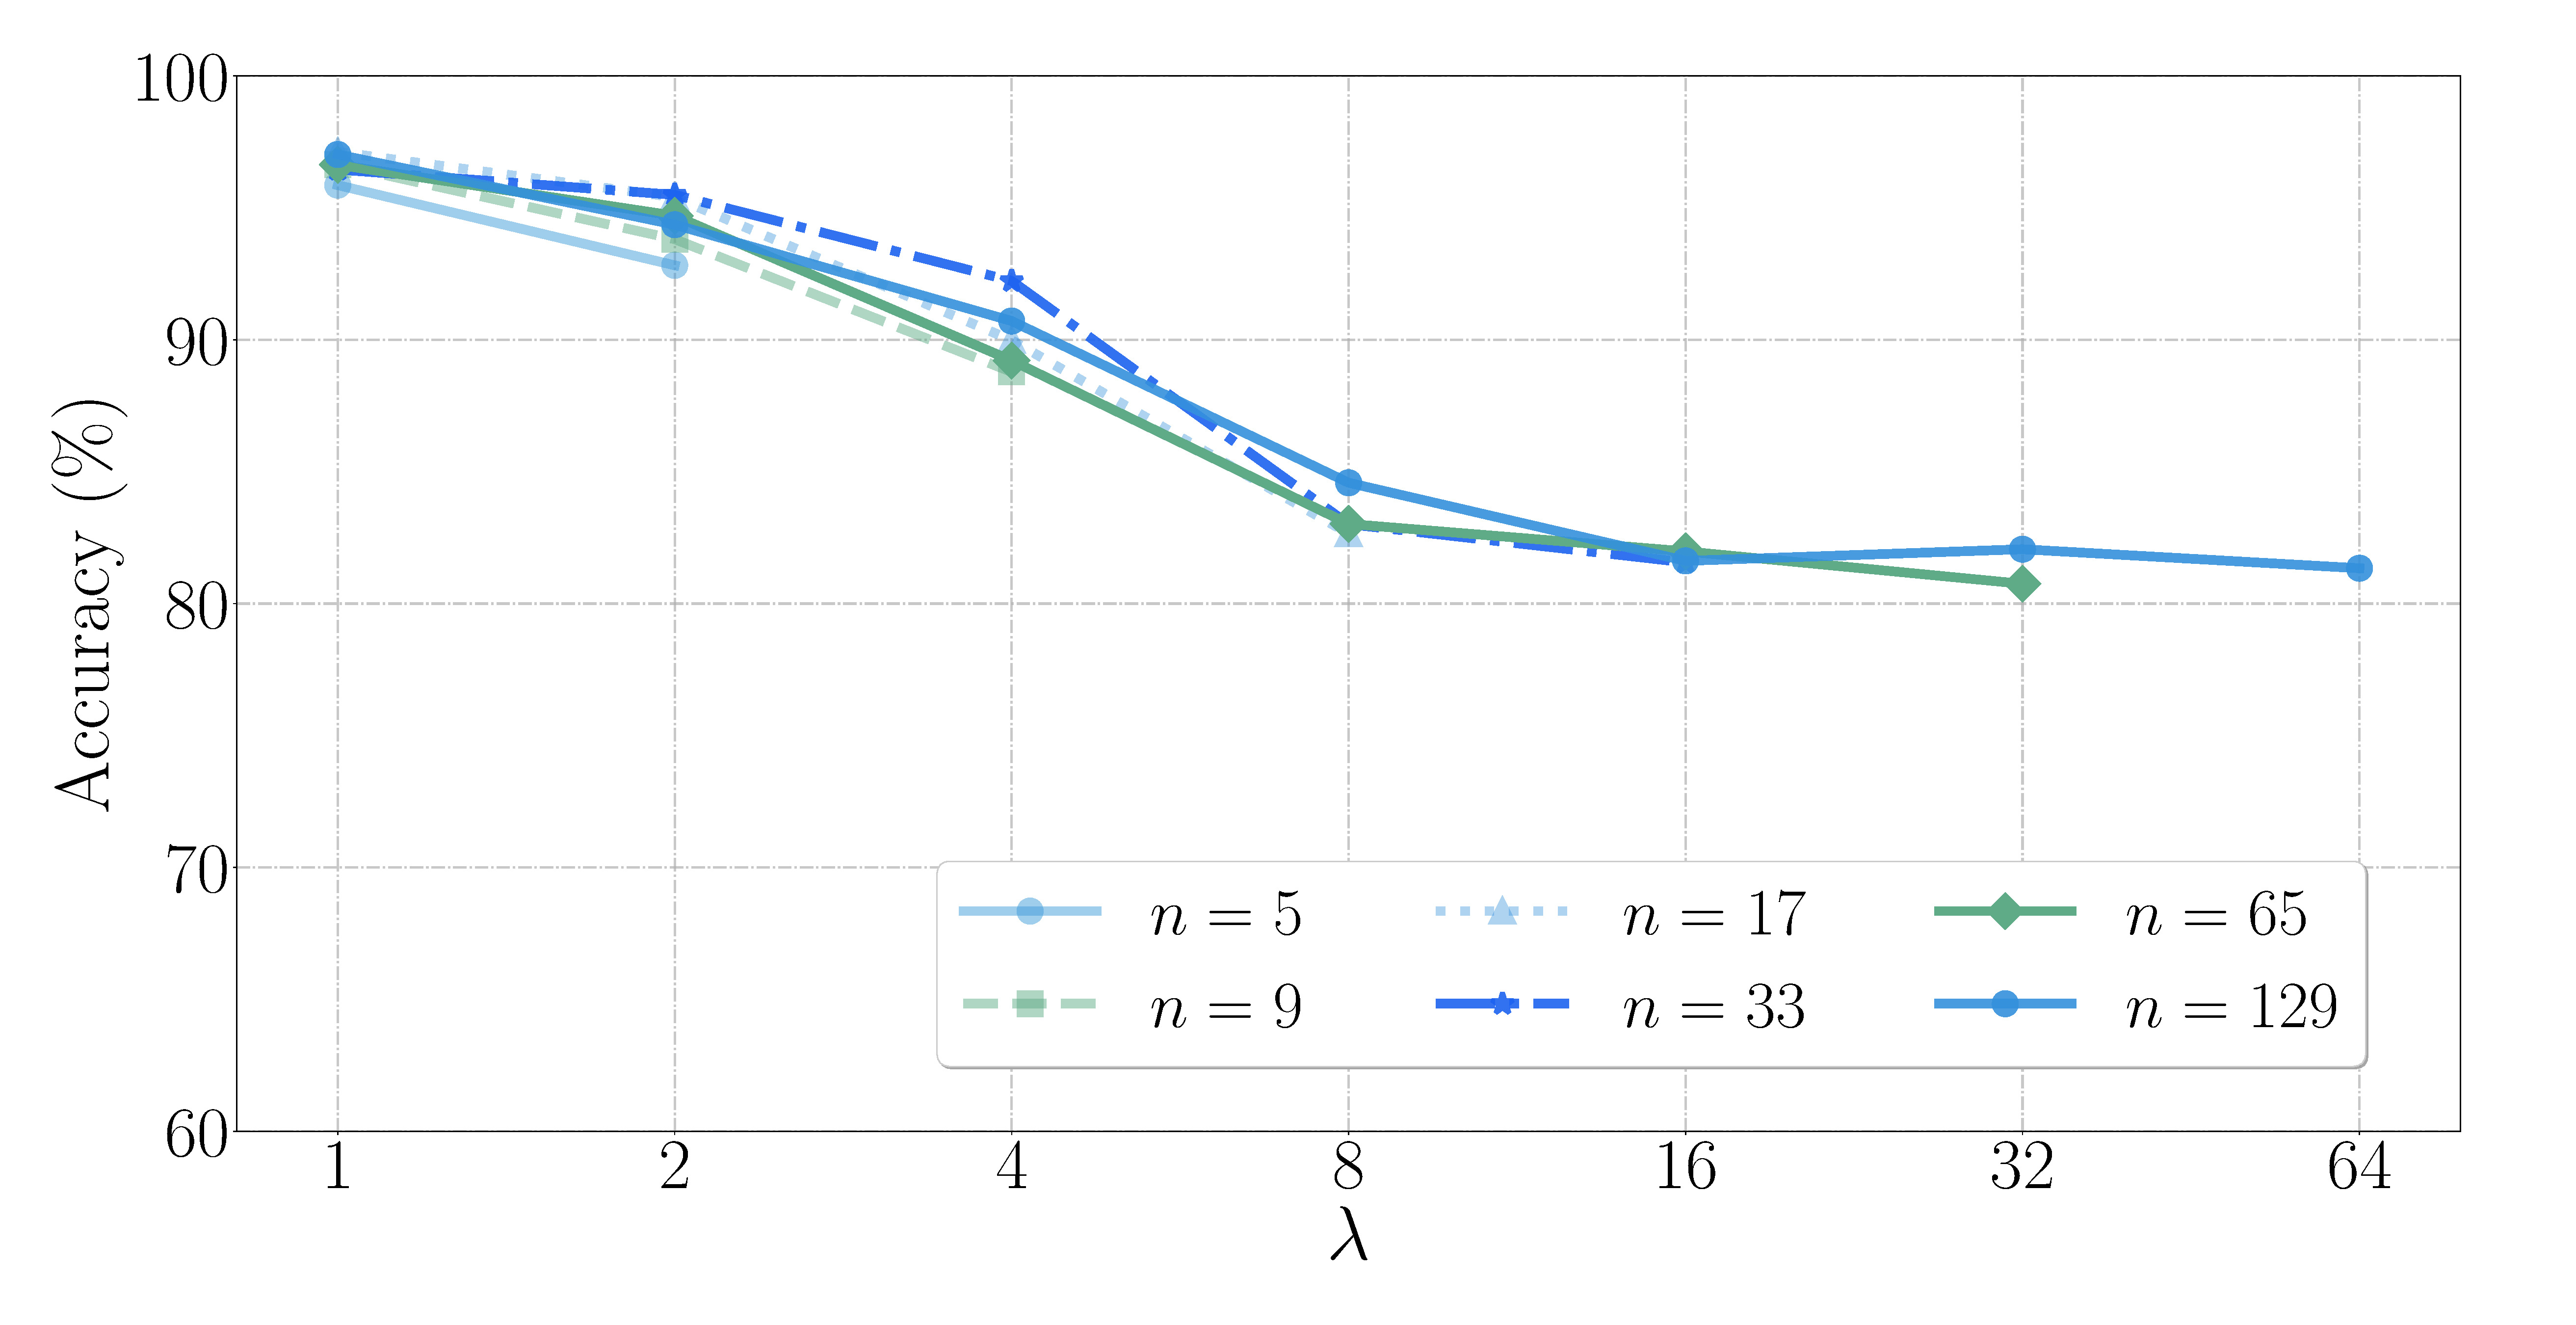
\includegraphics[width=0.56\linewidth]{latex/eval/DR_m.pdf}
    \caption{Accuracy of the feedback algorithm for different $\lambda$ and $n$ values when Byzantine models collude.}
    \label{fig:dr_m}   
    \vspace{-15pt}
\end{figure}

\section{Necessity Analysis of Liveness}
We further analyze the necessity of the liveness property. In real-world deployments, the goal of $\mathcal{MG}$ is not only to guarantee safety, but also to accomplish normal inference tasks such as mathematics, medical diagnosis, and programming. The objective is to maintain both functionality and safety, rather than prioritize safety as the sole consideration. As a result, in practical applications, $\mathcal{MG}$ must be able to perform valid reasoning on a wide variety of prompts. From the perspective of safety, abstention can be used to avoid unsafe responses. However, for regular inference tasks, abstention is not acceptable, as the response $\bot$ cannot adaptively provide reasonable outputs for unknown prompts. Therefore, liveness is necessary for $\mathcal{MG}$ from a practical application perspective. 

\end{document}
